% !TEX root = NotesDeCours.tex

% ================================================================================================ 
% Page de titre :
% ================================================================================================

\begin{frame}

  \color{bleu}

  \begin{flushleft}
    
    \Large
   	\bf
    
    Mécanique des fluides 

  \end{flushleft}
  
  \ligne{3} % remplace: \noindent \thickline{0.5mm}{150}

  \begin{flushright}

    \rm

    \textrm{David} \textsc{Fabre}
    
    \vspace{3mm}
    
    IMFT / UPS
    
    Département de Mécanique
    
    david.fabre@imft.fr

  \end{flushright}


 % \begin{picture}(110, 30)(10, -20)
  %  \put( 20, -20){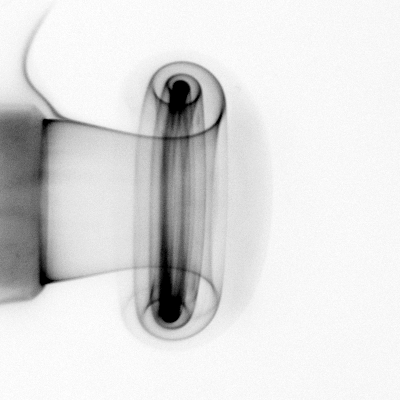
\includegraphics[height=45mm]{./Figures/vortex_ring_Re400_white.png}}
 %   \put(67, -12){\color{gris} \small \slshape Anneau tourbillonnaire}    	
   % \put(67, -15){\color{gris} \small \slshape généré par piston}
   % \put(67, -19){\color{gris} \small \copyright\,\! IMFT}
 % \end{picture}

\begin{picture}(110, 30)(9, -18)
  \put( 15, -22){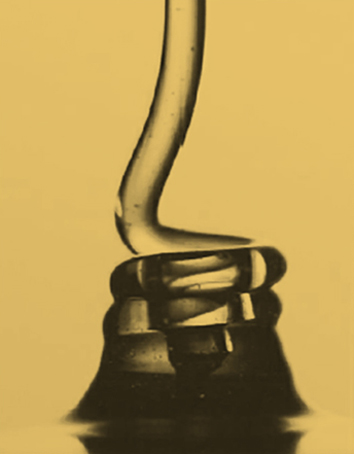
\includegraphics[height=30mm]{./Figures/miel1.jpg}}
  \put( 40, -22){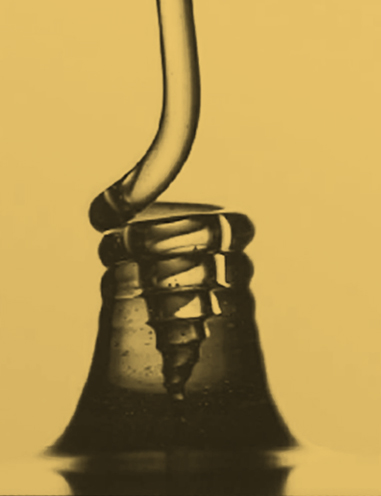
\includegraphics[height=30mm]{./Figures/miel2.jpg}}
  \put( 64.5, -22){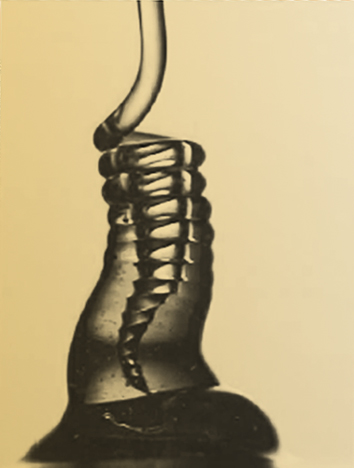
\includegraphics[height=30mm]{./Figures/miel3.jpg}}
  \put( 89, -22){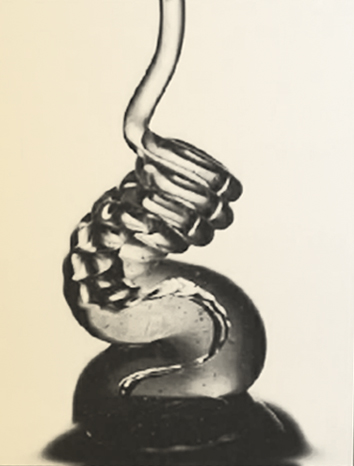
\includegraphics[height=30mm]{./Figures/miel4.jpg}}
  \put(16, -25){\color{gris} \small \rm Enroulement d'un filet de miel. Patricia ERN \copyright\ IMFT}
\end{picture}
  \vspace{7mm}
  

  \vspace{5mm}
  
  \begin{flushright}
    
    \Large
   	\bf
    
    4. Viscosité et Rhéologie

  \end{flushright}

\end{frame}

%%%%%%%%%%%%%%%%%%%%%%%%%%%%%%%%%%%%%%%%%%%%%%%%%%%%%%%%%%%%%%%%%%%%%%%%%%%%%%%%%%%%%%%%%%
% Sommaire :
%%%%%%%%%%%%%%%%%%%%%%%%%%%%%%%%%%%%%%%%%%%%%%%%%%%%%%%%%%%%%%%%%%%%%%%%%%%%%%%%%%%%%%%%%%



\begin{frame}{Sommaire}

\small
  
\hspace*{2mm}
\begin{tabular}{cc}
		%&
  		\begin{minipage}{62mm}
  			\tableofcontents[firstsection=0]
      \vspace{15mm}
  		\end{minipage}
  		&   
  		\begin{minipage}{60cm}
		  \vspace*{-5mm}  
  			%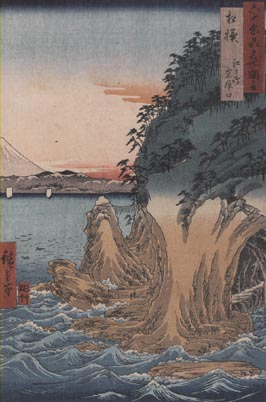
\includegraphics[width=40mm]{vagues.jpg} 
  		\end{minipage}
  	\end{tabular}

\vspace{0mm}

\end{frame}




%%%%%%%%%%%%%%%%%%%%%%%%%%%%%%%%%%%%%%%%%%%%%%%%%%%%%%%%%%%%%%%%%%%%%%%%%%%%%%%%%%%%%%%%%%%%%%%%%%%
\section{Viscosité et Rhéologie}
%%%%%%%%%%%%%%%%%%%%%%%%%%%%%%%%%%%%%%%%%%%%%%%%%%%%%%%%%%%%%%%%%%%%%%%%%%%%%%%%%%%%%%%%%%%%%%%%%%%

\subsection{Rhéologie}

\subsubsection{Définitions}

\begin{frame}{Definitions}

\small

\begin{itemize}

\item En plus d'une force normale (pression, chap. 2), on constate qu'un fluide en mouvement peut exercer sur une surface $\cal S$ 
 une {\color{red} force tangentielle}.

%\item %Mise en évidence expérimentale : deux plaques de surface $S$, séparées d'une distance $h$, l'une est entrainée à la vitesse  $U$ .
%(écoulement de cisaillement simple).

\item Commençons par caractériser cette force dans le cas simple d'un {\em écoulement plan parallèle} : 

$$
\vec{u} = u(y,t) \vec{e}_x
$$




\item {\bf Définition :} On appelle Contrainte Visqueuse $\tau_{{\color{red} x} {\color{blue} y}}$ 
la force tangentielle {\em Par unité de surface}, exercée {\color{red} dans la direction $x$} sur une facette d'orientation normale {\color{blue} y}, par le demi-espace $y^+$ sur le demi-espace $y^_-$.


$$d \vec{F}_{(y^+)\rightarrow (y^-)} = \left( - p \vec{e_y} + \tau_{xy} \vec{e_x} \right) dS$$

\item {\bf Définition :}  on appelle taux de cisaillement local la quantité $\dot \gamma = \frac{\partial u}{\partial y}$


\item {\bf Définition :} (pour un écoulement plan parallèle) on appelle {\em Loi rhéologique} la loi reliant $\tau_{xy}$ à $\dot \gamma $.
 
\item 
Remarque importante : tout comme la pression, la contrainte visqueuse s'exerce à la fois sur une paroi solide 
ou sur une surface (fictive) séparant le fluide en deux sous-domaines.

\end{itemize}


\end{frame}


\subsubsection{Cas des gaz}

\begin{frame}{Cas des gaz}

\small
\bigskip

Pour les gaz, on observe une loi rhéologique {\em linéaire } (ou Newtonienne).

$$ \tau_{xy} = \mu \dot{ \gamma} $$

$\mu$ = viscosité cinématique.

\pause
\medskip


Explication physique : Illustrations avec le programme {\sc kinetics.m}.


La contrainte visqueuse est due :

\begin{itemize}
\item
 (entre deux volumes fluides adjacents) {\em aux échanges de quantité de mouvement tangentielle due aux transferts de particules
 venant de régions de vitesse moyenne (au sens MMC) différentes.}
 \item
 (sur une surface solide) {\em aux variations de quantité de mouvement tangentielle dues aux collisions sur la paroi}
\end{itemize}




\pause 
\smallskip 
$=>$  Dans un gaz la viscosité augmente avec la température (cad avec l'agitation thermique). 


(Loi de Sutherland : $\mu \approx \mu_0 (T/T_0)^{3/2}$)





\pause
\medskip
Remarque sur les {\em conditions limites } :

\medskip

Une paroi est elle-même constituée de particules en agitation thermique ... Après chaque collision les particules sont renvoyées
dans des directions aléatoires. 
\smallskip 
Pour une paroi fixe en $y=0$ : 

$$ u_x(y=0) = 0$$ 

Généralisation : 

\smallskip 
Pour une paroi de vitesse $U_{paroi}$ en $y=y_{paroi}$, $u(y_{paroi}) = U_{paroi}$.

On appelle cette condition une {\em condition limite d'adhérence }.


\end{frame}


\subsubsection{Cas des liquides "simples"}
\begin{frame}{Cas des liquides simples}

\small
\bigskip

Liquides "simples" = constitués de "petites molécules" (eau, huiles, métaux liquides, etc...)

\bigskip

On observe également une loi rhéologique linéaire : $\tau_{xy} = \mu \dot{\gamma}$ (loi Newtonienne).

\smallskip
Explication physique : pour mettre en mouvement les strates de fluide les unes par rapport aux autres, il faut briser des liaisons pour en recréer d'autres.

\bigskip


C'est d'autant plus facile que l'agitation thermique est importante

\smallskip
$=>$ Dans un liquide (simple),  la viscosité diminue avec la température !

\smallskip
(Loi de Suttner pour l'eau : $\mu = \mu_0 e^{-\alpha (T-T_0)}$ ).



\pause
\bigskip
Remarque sur les {\em conditions limites } :

L'étude des interactions entre particules fluides et molécules constituant une paroi solide justifient également
une {\em condition limite d'adhérence }

\smallskip 
$$
u(y_{paroi}) = U_{paroi}
$$




\end{frame}

\subsubsection{Cas des liquides "complexes"}
\begin{frame}{Cas des liquides "complexes"}
\small
\bigskip

Pour des liquides "complexes" (mélanges, suspensions, contenant des "grosses" molécules ou particules) on observe des comportements divers :
\pause \smallskip

%Quelques exemples :

$$
\includegraphics[width=.35\linewidth]{../FIGURES/rheogramme.jpg}
$$

\pause \smallskip

\begin{itemize}

\item %Suspensions de particules allongées ou de polymères (shampooing, lessive, jus de fruits concentrés, encres d'imprimerie,...)
%On constate que la viscosité effective $\tau_{xy}/\dot{\gamma}$ {\em diminue}  avec $\dot{\gamma}$.
Fluides rhéo-fluidifiants (shear-thinning) : la viscosité effective diminue avec le cisaillement.

Exemples : shampooing, lessive, jus de fruits concentrés, encres d'imprimerie,...

%(Explication physique : les particules "s'alignent" avec le cisaillement et offrent moins de résistance à la déformation.)

\item 
Fluides rhéo-épaississants (shear-thickenning) : la viscosité effective augmente avec le cisaillement.


Exemples : maïzena, suspensions diluées de polymères, ...

\item {\em Fluides à seuil}  (ou solides visco-plastiques) :
il faut exercer une contrainte minimale $\tau_c$ pour mettre le fluide en mouvement.

Exemples : boues, mayonnaise, ketchup,  dentifrice, cf. TD 4.1.

%\pause 
%$$
%|\tau_{xy}| \leq \tau_c \quad \longrightarrow \quad \cdot{ \gamma } = 0 \qquad  \mbox{ (mais } \gamma = dX/dy \ne 0 \mbox{ ; comportement de solide élastique). }
%$$  

%$$
%|\tau_{xy}| \geq \tau_c \quad \longrightarrow \quad |\tau{xy}|-\tau_c = f(\dot{\gamma} \qquad  \mbox{ ( loi } f(\gamma)  \mbox{ ; linéaire pour le modèle de Bingham). }
%$$  




%\pause 
%Explication physique : 



%M\item %Suspensions de particules allongées ou de polymères (shampooing, lessive, jus de fruits concentrés, encres d'imprimerie,...)

%On constate que la viscosité effective $\tau_{xy}/\dot{\gamma}$ {\em diminue}  avec $\dot{\gamma}$.

%On parle de fluides rhéofliuidifiants (shear-thinning)

%%Explication physique : les particules "s'alignent" avec le cisaillement et offrent moins de résistance à la déformation.

%\pause \smallskip
 
%\item  
%\item Suspensions de particules allongées ou de polymères (shampooing, lessive, jus de fruits concentrés, encres d'imprimerie,...)

%On constate que la viscosité effective $\tau_{xy}/\dot{\gamma}$ {\em diminue}  avec $\dot{\gamma}$.

%On parle de fluides rhéofliuidifiants (shear-thinning)

%Explication physique : les particules "s'alignent" avec le cisaillement et offrent moins de résistance à la déformation.

 

\end{itemize}




\end{frame}

%\begin{frame}{Bilan : lois rhéologiques classiques} 
%\end{frame}

\subsubsection{Compléments : lois rhéologiques instationnaires}
\begin{frame}{Compléments : lois rhéologiques instationnaires}

\small
\bigskip

Pour certains fluides on observe de plus que la loi rhéologique ne dépend pas seulement des valeurs instantanées de 
$\tau_{xy}$ et $\dot{\gamma}$ mais aussi de la  manière dont les contraintes et les déformations varient au cours du temps :

\begin{itemize}

\item Comportement thixotrope

La viscosité "effective" diminue avec la durée d'imposition de la contrainte.

Exemples : Terre agricole, boue, polymères, ...

\item Comportement viscoélastique 

Contraintes exercées "rapidement" $=>$ Comportement de solide élastique 

Contraintes exercées "lentement" $=>$ Comportement de fluide visqueux. 

Exemples : Maïzena, pâte silicone, ...


\end{itemize}



\end{frame}




\subsubsection{Généralisation : écoulements tridimensionnels}
 
\begin{frame}{Loi rhéologique pour un fluide Newtonien (cas général)}

\small

\bigskip

Généralisation : $\tau_{xy}$ et $\dot{\gamma}$ se généralisent en introduisant les tenseurs $\mytensor{\tau}$  et $\mytensor{D}$.

\medskip
\pause

On appelle {\em Loi rhéologique} la relation entre les tenseurs $\mytensor{\tau}$ et  $\mytensor{D}$.

\medskip
\pause

On appelle \textbf{fluide newtonien} un fluide dont la loi rhéologique est linéaire.



\medskip
\pause

Les principes de la MMC (symétrie, objectivité, etc...) imposent qu'une loi rhéologique linéaire 
est nécessairement de la forme :

\[
	\mytensor{\tau} = 2 \mu \, \mytensor{D'} + \mu^* \divergence(\myvec{u}) \mytensor{1}
\] 

où $\mu$ désigne la viscosité dynamique du fluide, $\mu^*$ la viscosité volumique (habituellement négligée),
$\mytensor{D'}$ est le déviateur du tenseur des taux de déformations donnés par
\[
\mytensor{D'} = \mytensor{D} - \frac{\divergence(\myvec{u})}{3}  \mytensor{1} ; 
\qquad 
	\mytensor{D} = \frac{1}{2}\, \left ( \ggradient\ \myvec{u} + \,^t\ggradient\ \myvec{u} \right )
\] 

Dans le cas d'un écoulement isovolume ($\divergence(\myvec{u}) = 0$) 
on l'écrira sous la forme plus simple :
\[
\mytensor{\tau} = 2 \mu \, \mytensor{D} 
\]
%\end{itemize}


\end{frame}

%%%%%%%%%%%%%%%%%%%%%%%%%%%%%%%%%%%%%%%%%%%%%%%%%%%%%%%%%%%%%%%%%
%
\subsection{Ecoulements plans parallèles de fluides Newtoniens}
%
%%%%%%%%%%%%%%%%%%%%%%%%%%%%%%%%%%%%%%%%%%%%%%%%%%%%%%%%%%%%%%%%%


\begin{frame}{Etablissement de l'équation}
\subsubsection{Equation des films visqueux}



\bigskip
\small
Considérons un écoulement {\em parallèle} , éventuellement instationnaire, 
d'un fluide {\em Newtonien}, {\em incompressible } décrit par son champ de vitesse 

$$ 
\vec{u} = u(y,t) \vec{e}_x 
$$


\pause
\medskip 

Par un bilan de quantité de mouvement  sur un volume élémentaire de fluide (projeté dans la direction $x$), on obtient l'équation des films visqueux 
(parfois appelée Equation de Navier) :


$$
\rho \frac{\partial u}{\partial t} = \rho g_x - \left[ \frac{\partial p}{\partial x} \right] + \mu \frac{\partial^2 u}{\partial y^2} 
$$ 

\pause
\medskip 

Remarques :
\begin{enumerate}

\item Autre forme possible de l'équation :
$$
\frac{\partial u}{\partial t} = g_x - \left[ \frac{1}{\rho} \frac{\partial p}{\partial x} \right] + \nu \frac{\partial^2 u}{\partial y^2} 
$$ 


\item On peut justifier que le gradient de pression est nécessairement uniforme:
 $\left[ \frac{\partial p}{\partial x} \right] = C_{te} = \frac{[P(L)-P(0)]}{L}$ \qquad {\color{vert} [Démonstration :]}
  


\item
Conditions limites :

\begin{itemize} 
\item Sur une surface solide de vitesse $U_p$ :

$ u(y_p) = U_p$ (Condition d'adhérence.) 

\item Sur une surface libre (liquide/gaz de masse volumique négligeable) :

$\tau_{xy} = 0  \qquad \rightarrow \frac{\partial u}{\partial y} = 0$ (Condition de contrainte nulle).

%\item (Remarque : sur une surface entre deux liquides :)  $\tau_{xy}$ est continue 

\end{itemize}

\end{enumerate}



\end{frame}



%\begin{frame}{Conditions limites}
%\end{frame}

\subsubsection{Solutions classiques stationnaires (rappels L2)}

\begin{frame}{Solutions classiques stationnaires (rappels L2)}

\begin{center}
			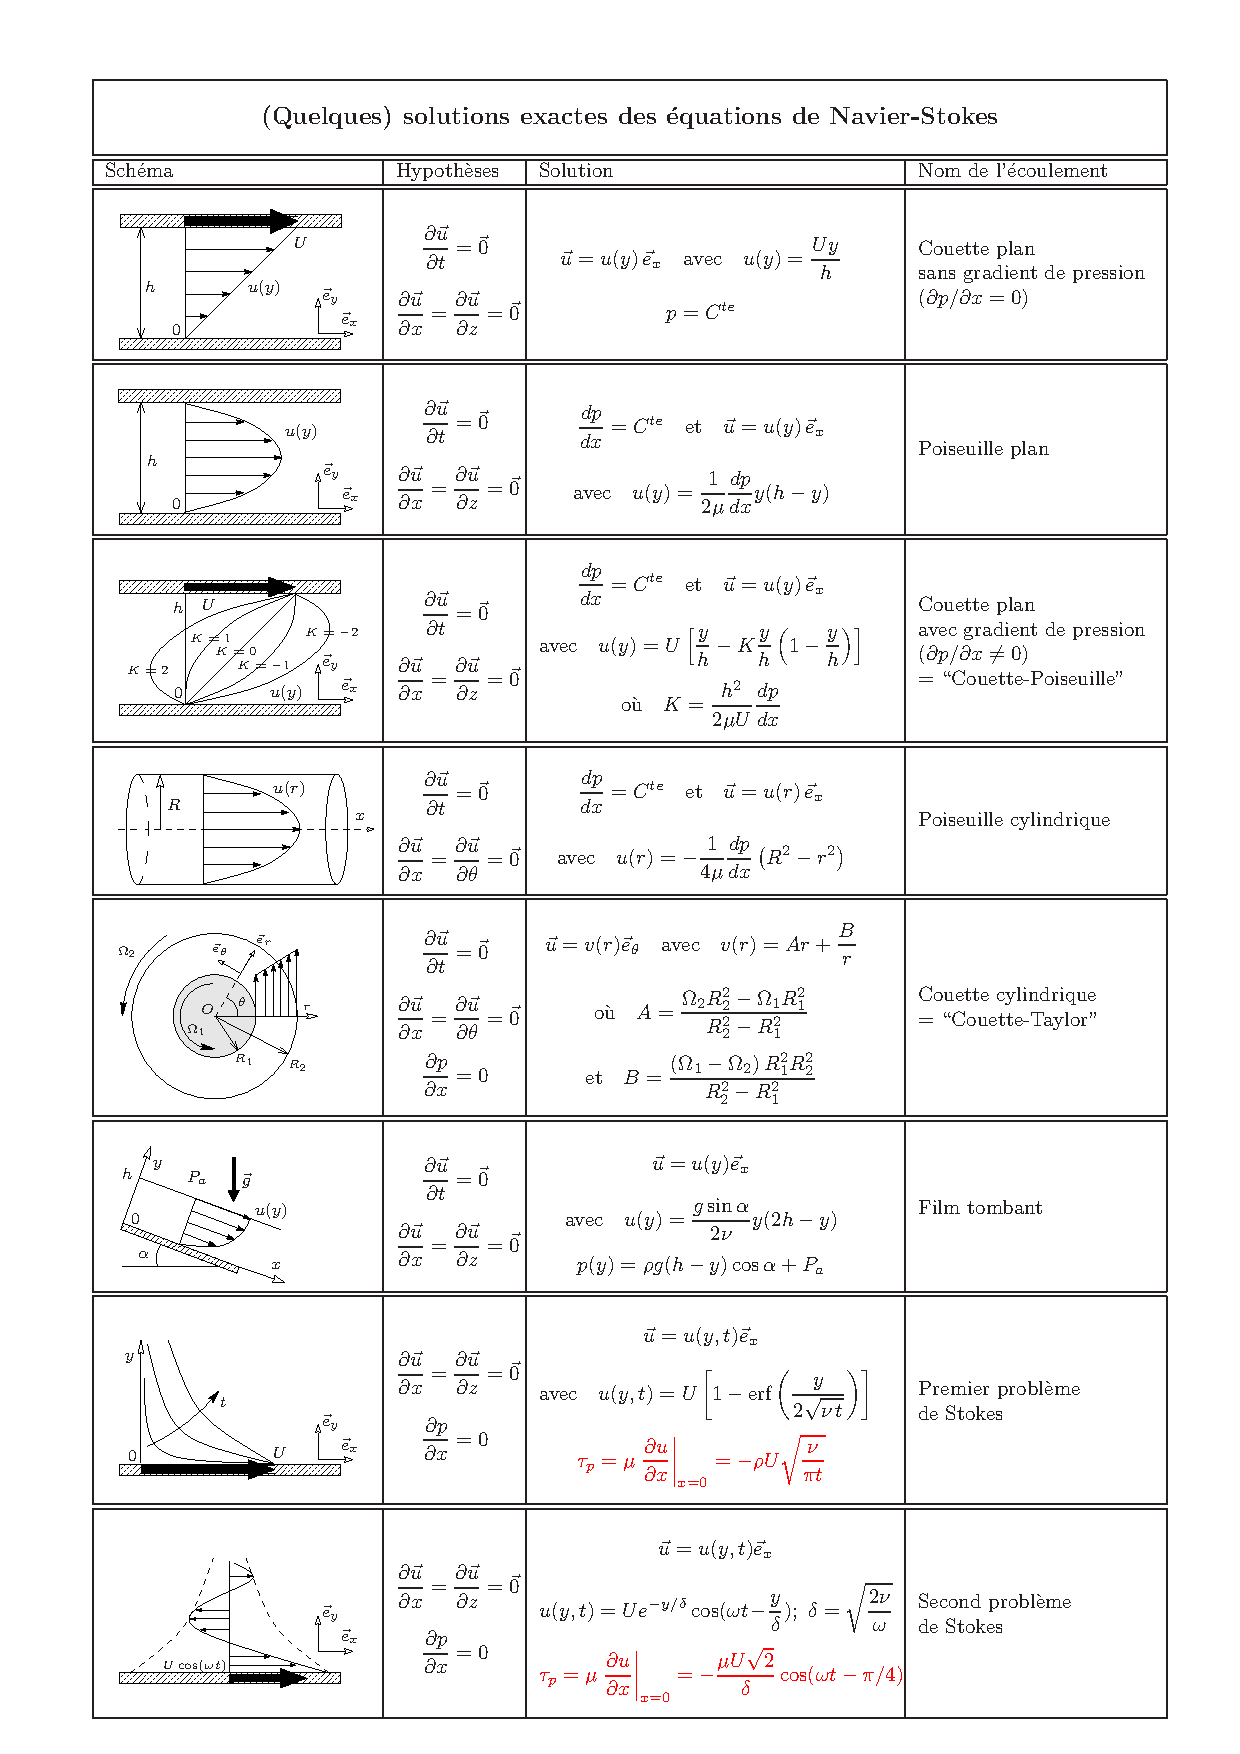
\includegraphics[height=10.8cm]{solutions_exactes_D}
\end{center}



\end{frame}


\subsubsection{Problèmes instationnaires}
%\begin{frame}{1er problème de Stokes}

%{\bf Problème : } Mise en mouvement d'un fluide par mouvement impulsionnel d'une paroi solide



%=> Observation : existence 
%d'un 

%\end{frame}

%--------------------------------------------------------------------------------------------------
\begin{frame}{Problème : plaque en translation dans un fluide visqueux}
%--------------------------------------------------------------------------------------------------

\small

{\bf 1er Problème de Stokes : } à $t=0$, l'écoulement est au repos ; pour  $t >0$ la paroi ($y=0)$ est mise en mouvement à la vitesse constante $U$.
 
 (illustrations avec le programme {\sf kinetics.m} ).
  
 

\begin{overprint}

  \onslide<1>   

  \begin{center}
    \begin{picture}(100, 50)
    \put( 0, 0){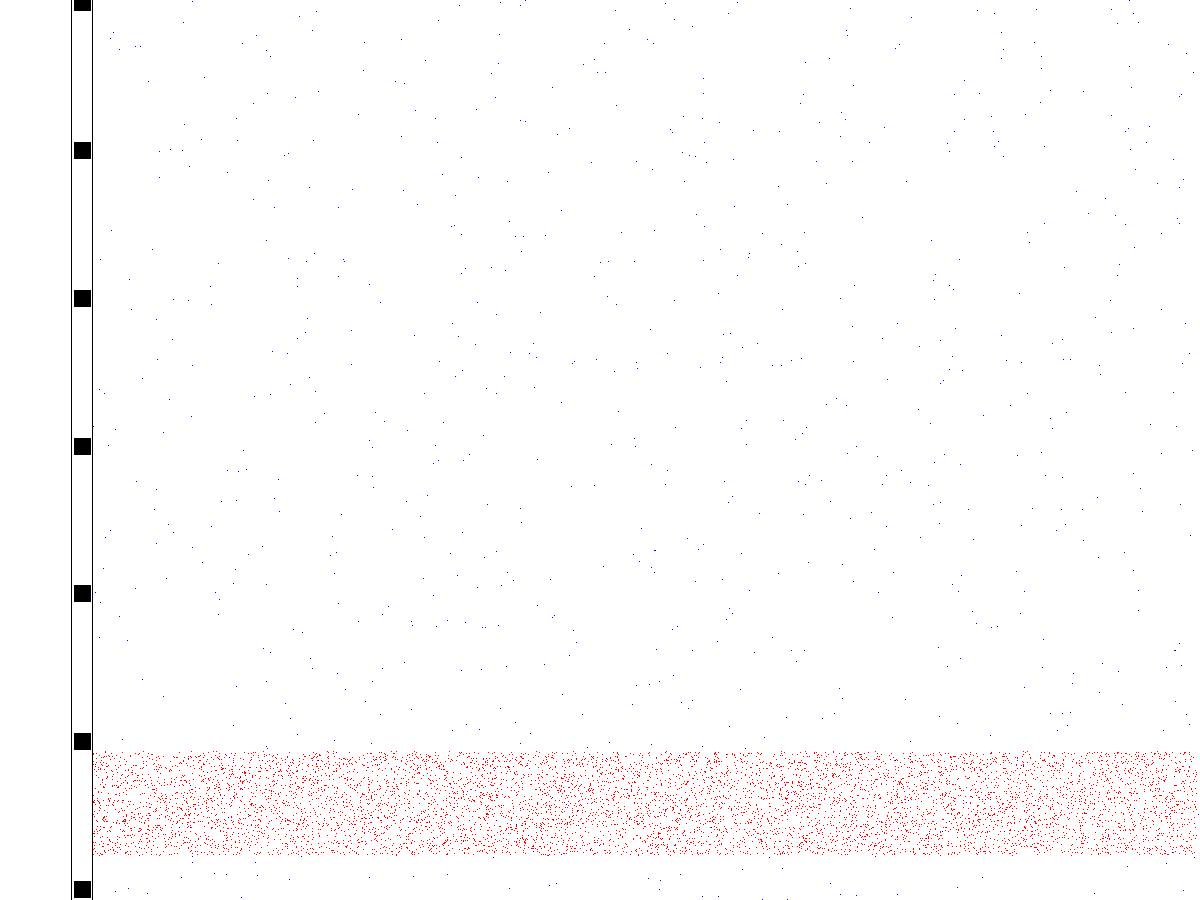
\includegraphics[width=50mm]{momentum_diffusion_particles0.png}}
    \put(40, 40){$t=0^-$}
    \put(10, 22){$U_0=0$}
    \end{picture}
  \end{center}

  \onslide<2>   
  \begin{center}
    \begin{picture}(100, 50)
    \put( 0, 0){\movie[width=50mm,poster,externalviewer,showcontrols=false]{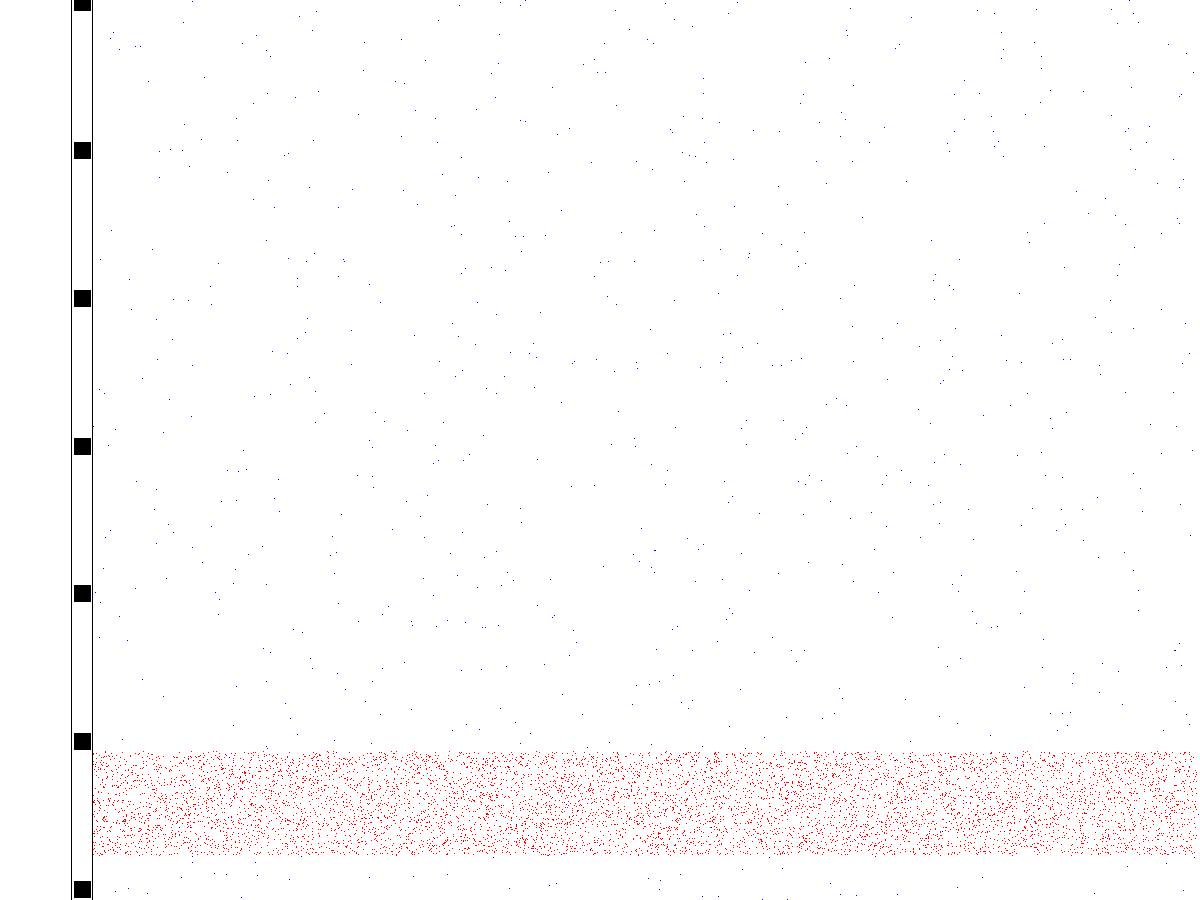
\includegraphics[width=50mm]{momentum_diffusion_particles0.png}}{./Figures/momentum_diffusion.avi}}
    \put(40, 40){$t=0^+$}
    \put(1,0){\vector(0, 1){20}}
    \put(-1, 28){$U_1$}
    \put(0, 25){\rotatebox{90}{$=$}}
    \put(-2, 22){$Cte$}
    \put(10, 22){$U_0=0$}
    \end{picture}
  \end{center}

  \onslide<3>   
  \begin{center}
    \begin{picture}(100, 50)
    \put( 0, 0){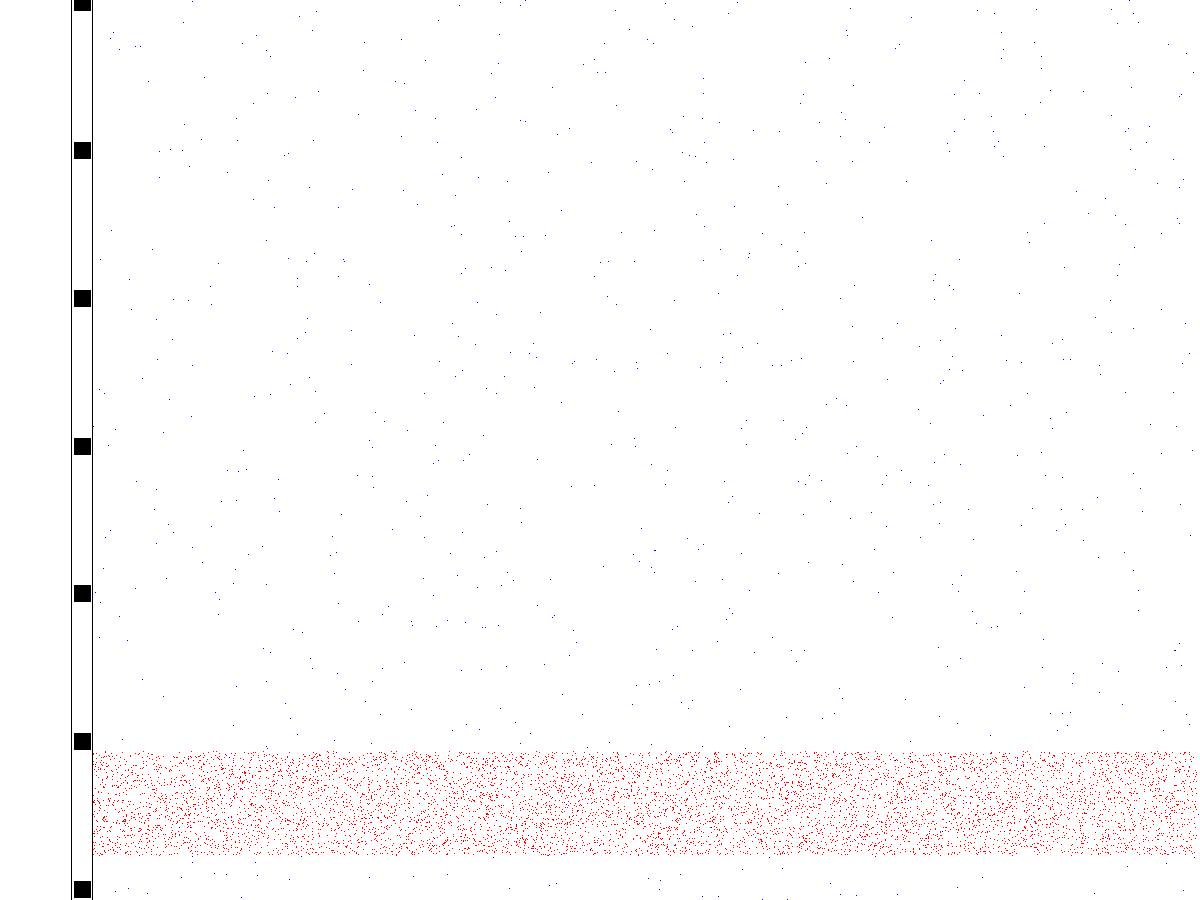
\includegraphics[width=50mm]{momentum_diffusion_particles0.png}}
    \put(55, 20){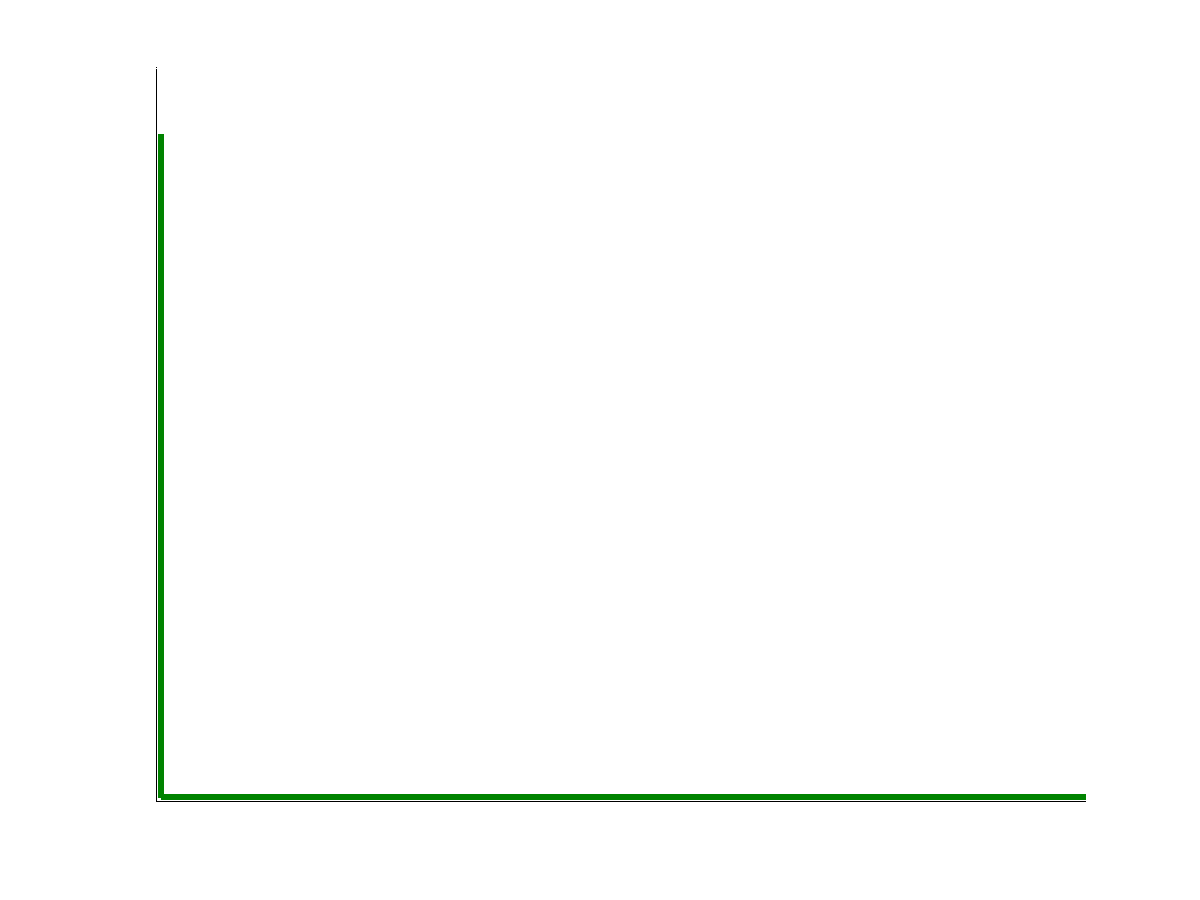
\includegraphics[width=45mm]{momentum_diffusion_profile0.png}}
    \put(60.9, 51.2){\linethickness{0.01mm}\line(1, 0){34.75}}
    \put(95.75, 51.2){\linethickness{0.01mm}\line(0, -1){27.5}}
    \put(59, 23){$0$}
    \put(97, 23){$x$}
    \put(57, 48){$U_1$}
    \put(83, 46){$u(y, t)$}
    \put(40, 40){$t=0^+$}
    \put( 4, 10){\color{vert} \line(1, 0){46}}
    \put(54, 10){\line(1, 0){10}}
    \put(64, 10){\vector(1, 1){10}}
    \put(73, 15){mesure du profil de}
    \put(72, 12){vitesse verticale $u(y, t)$}
    \put(1,0){\vector(0, 1){20}}
    \put(-1, 28){$U_1$}
    \put(0, 25){\rotatebox{90}{$=$}}
    \put(-2, 22){$Cte$}
    \end{picture}
  \end{center}

  \onslide<4>   
  \begin{center}
    \begin{picture}(100, 50)
    \put( 0, 0){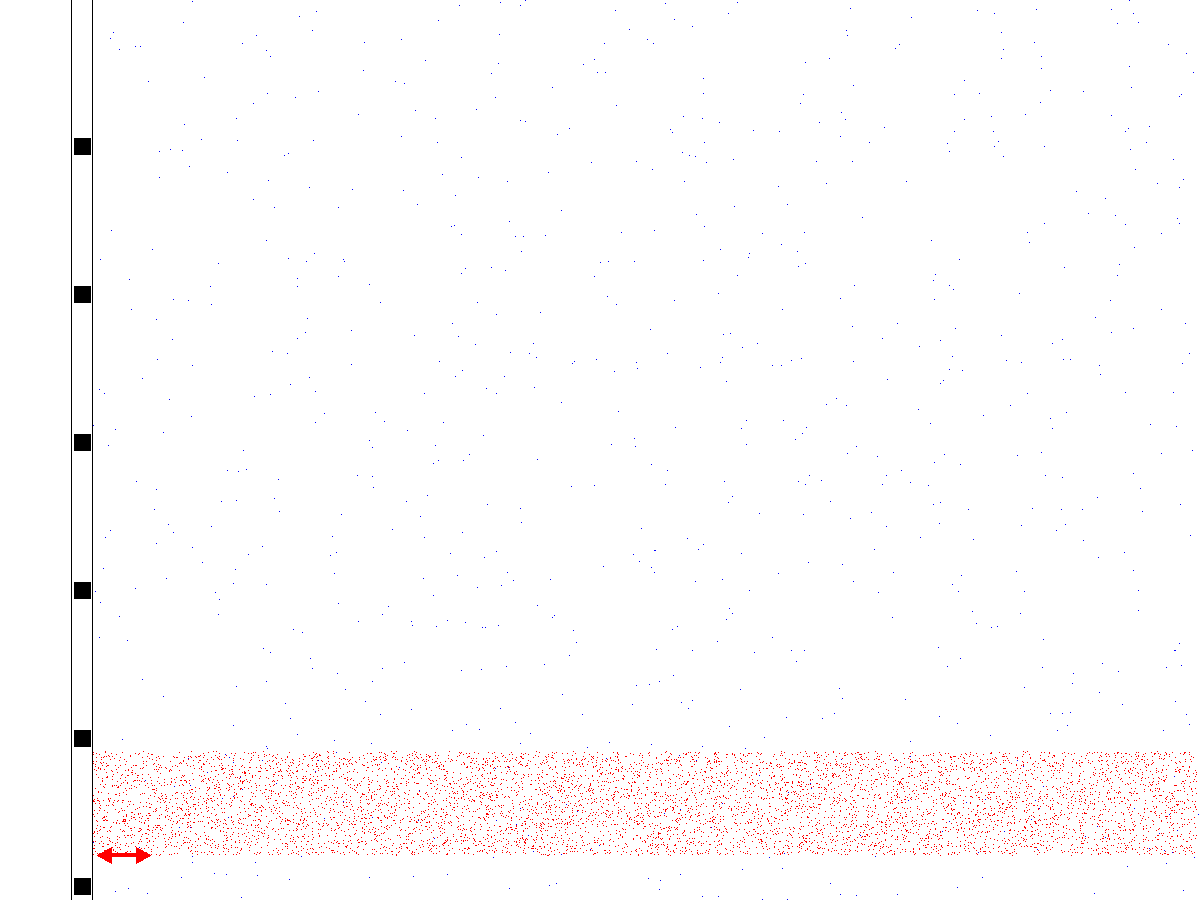
\includegraphics[width=50mm]{momentum_diffusion_particles1.png}}
    \put(55, 20){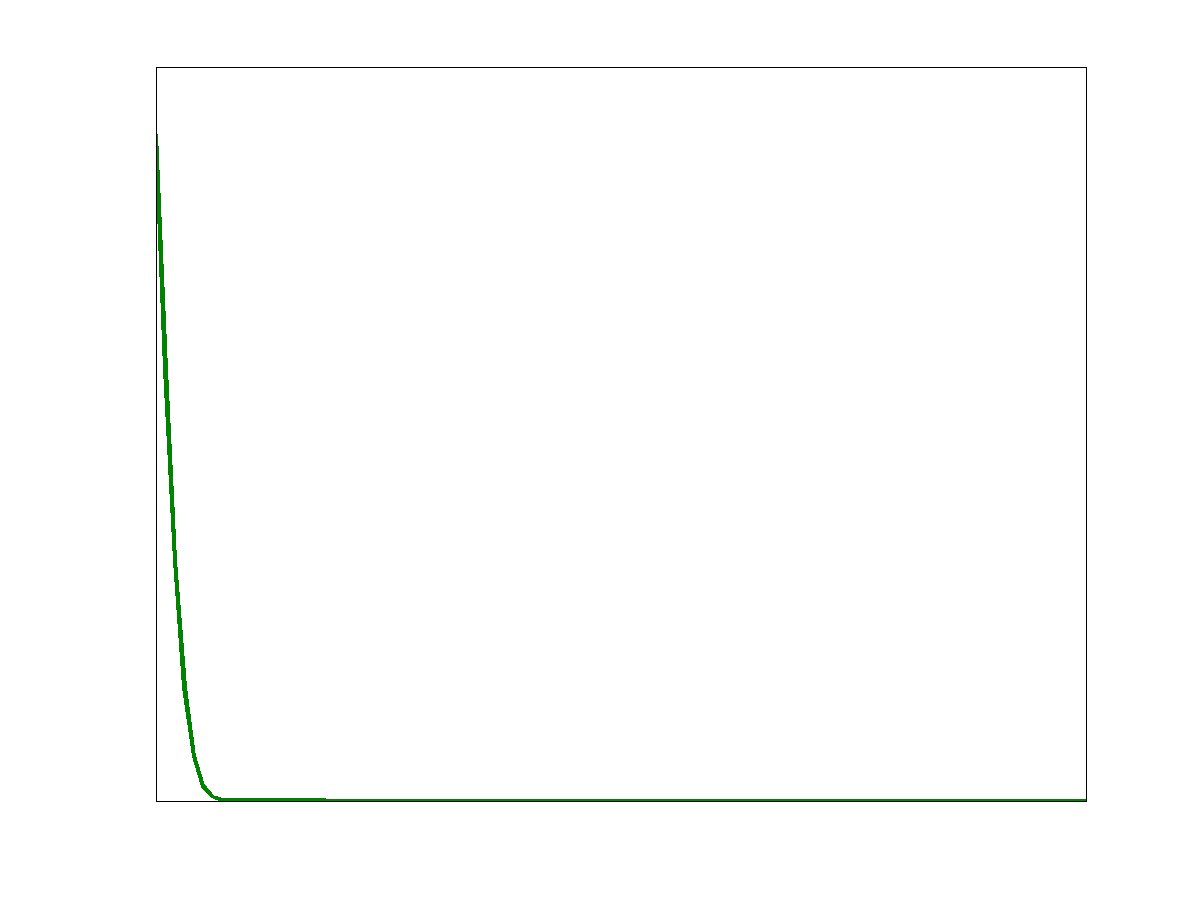
\includegraphics[width=45mm]{momentum_diffusion_profile1.png}}
    \put(60.9, 51.2){\linethickness{0.01mm}\line(1, 0){34.75}}
    \put(95.75, 51.2){\linethickness{0.01mm}\line(0, -1){27}}
    \put(59, 23){$0$}
    \put(97, 23){$x$}
    \put(57, 48){$U_1$}
    \put(83, 46){$u(y, t)$}
    \put(40, 40){$t=t_1$}
    \put( 4, 10){\color{vert} \line(1, 0){46}}
    \put(54, 10){\line(1, 0){10}}
    \put(64, 10){\vector(1, 1){10}}
    \put(73, 15){mesure du profil de}
    \put(72, 12){vitesse verticale $u(y, t)$}
    \put(1,0){\vector(0, 1){20}}
    \put(-1, 28){$U_1$}
    \put(0, 25){\rotatebox{90}{$=$}}
    \put(-2, 22){$Cte$}
    \put(62.3,25){\color{rouge} \vector(1, 0){0} \scriptsize $\delta(t_1)$}
    \put(4.5, 0){\color{rouge} \scriptsize $\delta(t_1)$}
    \end{picture}
  \end{center}

  \onslide<5>   
  \begin{center}
    \begin{picture}(100, 50)
    \put( 0, 0){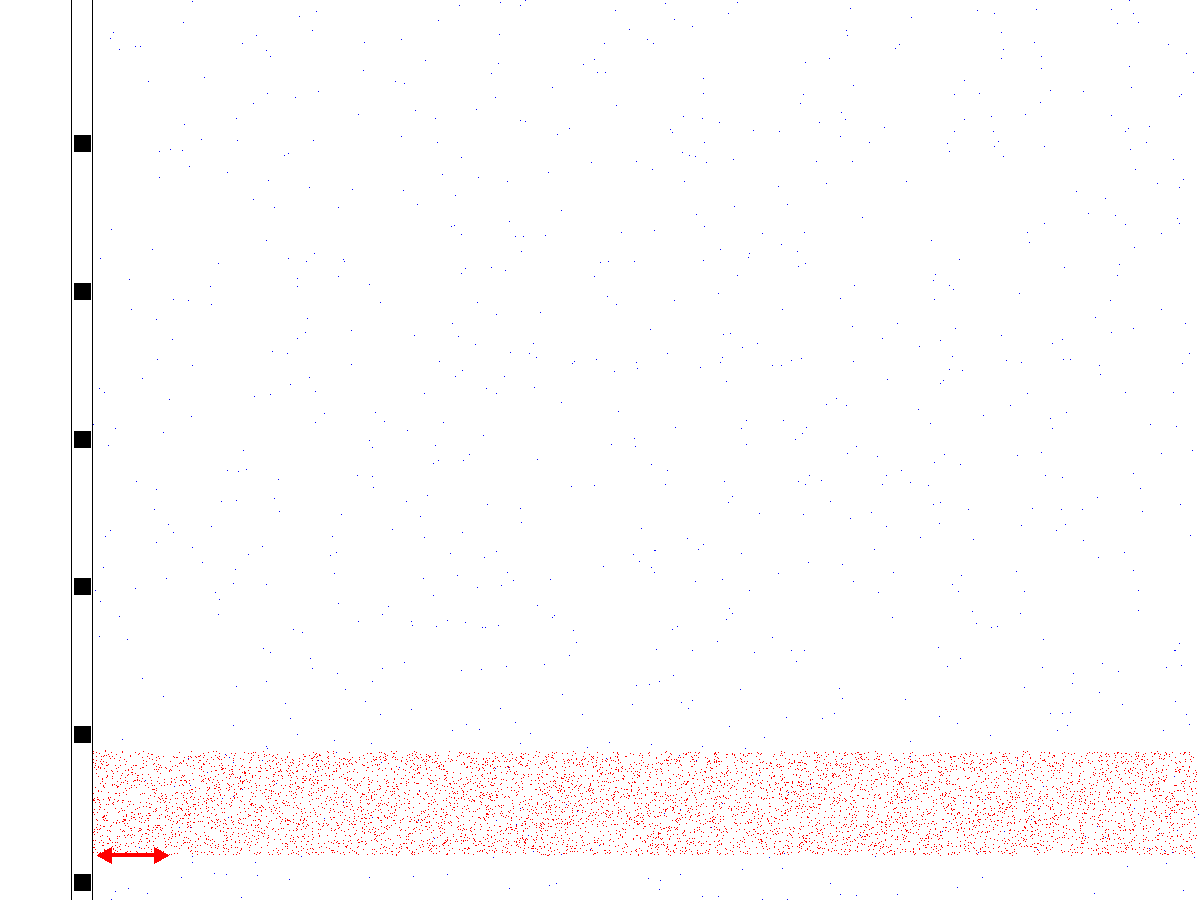
\includegraphics[width=50mm]{momentum_diffusion_particles2.png}}
    \put(55, 20){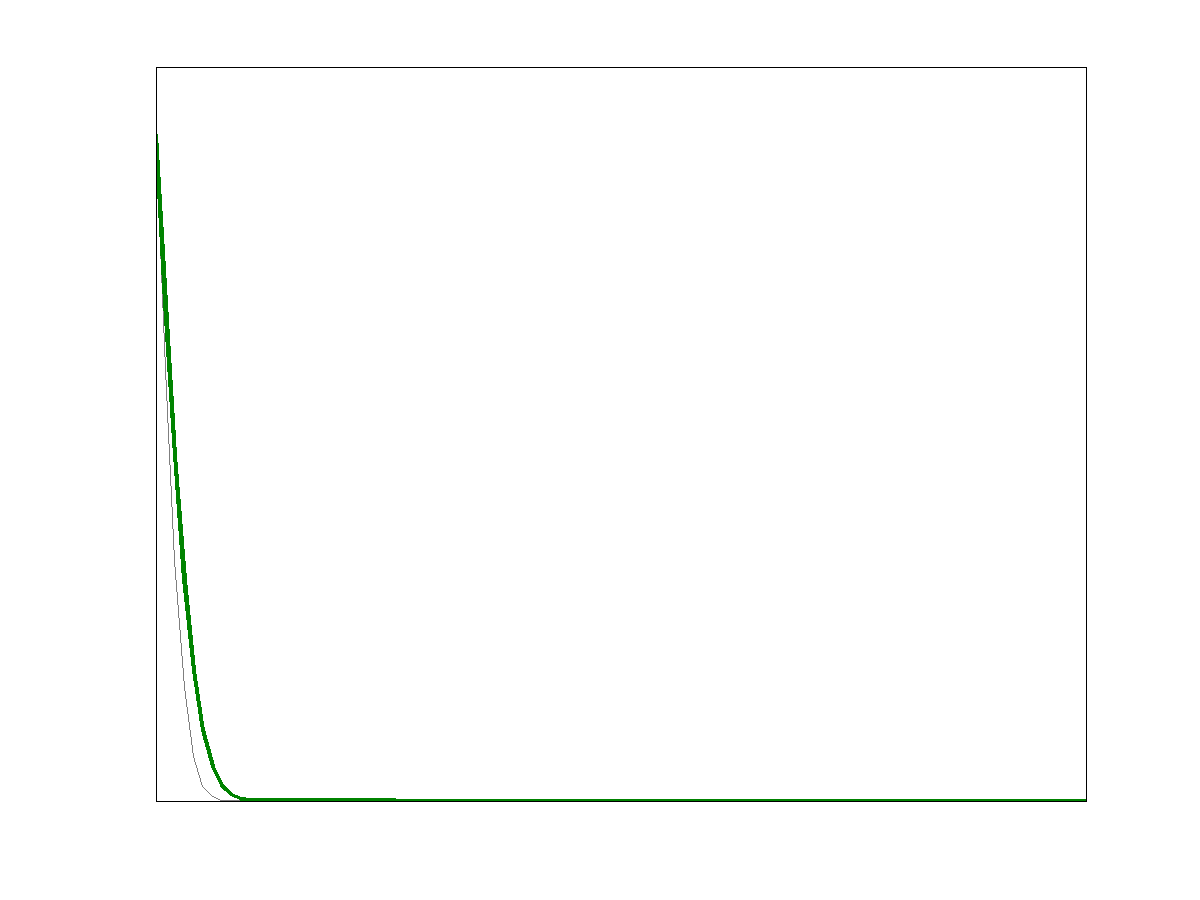
\includegraphics[width=45mm]{momentum_diffusion_profile2.png}}
    %\put(60.9, 51.2){\linethickness{0.01mm}\line(1, 0){34.75}}
    \put(59, 23){$0$}
    \put(97, 23){$x$}
    \put(57, 48){$U_1$}
    \put(83, 46){$u(y, t)$}
    \put(40, 40){$t=t_2$}
    \put( 4, 10){\color{vert} \line(1, 0){46}}
    \put(54, 10){\line(1, 0){10}}
    \put(64, 10){\vector(1, 1){10}}
    \put(73, 15){mesure du profil de}
    \put(72, 12){vitesse verticale $u(y, t)$}
    \put(1,0){\vector(0, 1){20}}
    \put(-1, 28){$U_1$}
    \put(0, 25){\rotatebox{90}{$=$}}
    \put(-2, 22){$Cte$}
    \put(61,25){\color{rouge} \vector(1, 0){2} \scriptsize $\delta(t_2)$}
    \put(4.5, 0){\color{rouge} \scriptsize $\delta(t_2)$}
    \end{picture}
  \end{center}

  \onslide<6>   
  \begin{center}
    \begin{picture}(100, 50)
    \put( 0, 0){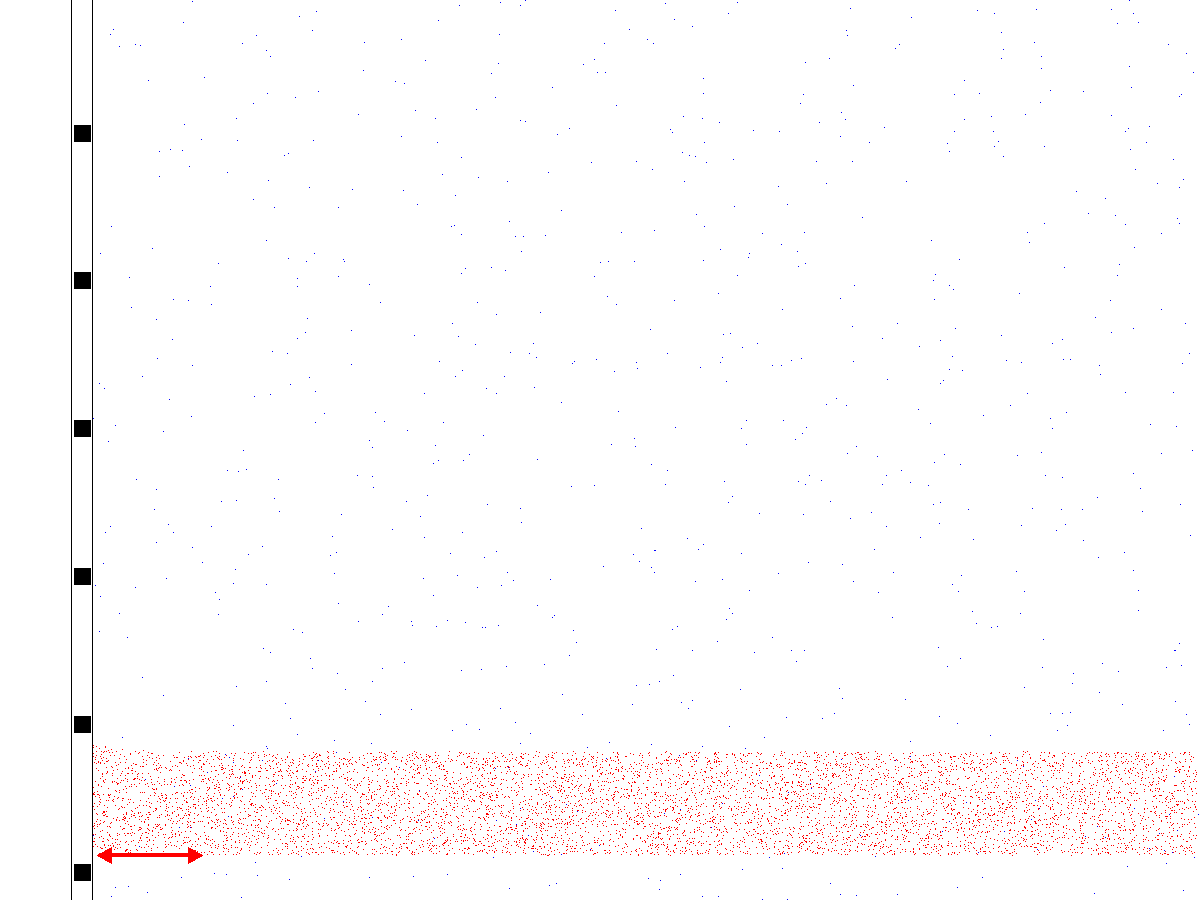
\includegraphics[width=50mm]{momentum_diffusion_particles3.png}}
    \put(55, 20){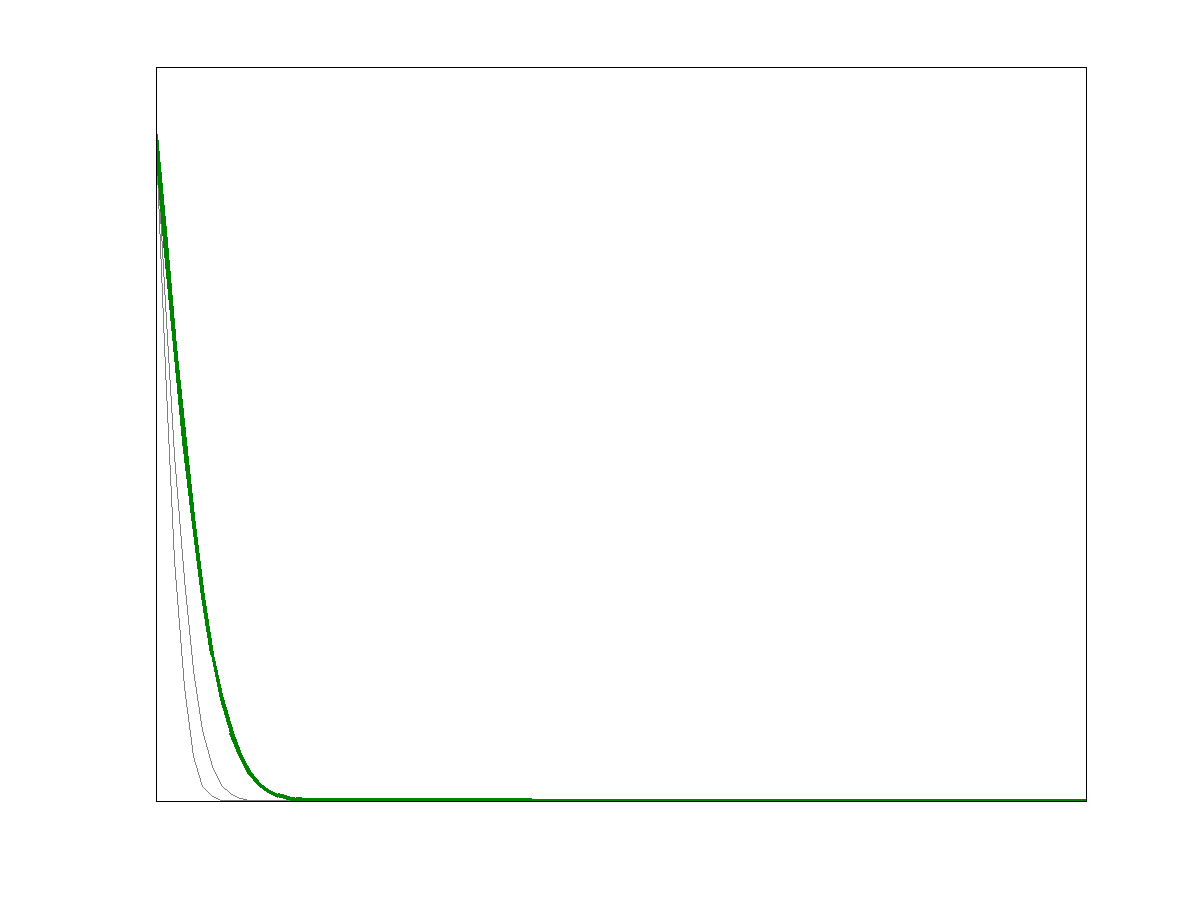
\includegraphics[width=45mm]{momentum_diffusion_profile3.png}}
    %\put(60.9, 51.2){\linethickness{0.01mm}\line(1, 0){34.9}}
    \put(59, 23){$0$}
    \put(97, 23){$x$}
    \put(57, 48){$U_1$}
    \put(83, 46){$u(y, t)$}
    \put(40, 40){$t=t_3$}
    \put( 4, 10){\color{vert} \line(1, 0){46}}
    \put(54, 10){\line(1, 0){10}}
    \put(64, 10){\vector(1, 1){10}}
    \put(73, 15){mesure du profil de}
    \put(72, 12){vitesse verticale $u(y, t)$}
    \put(1,0){\vector(0, 1){20}}
    \put(-1, 28){$U_1$}
    \put(0, 25){\rotatebox{90}{$=$}}
    \put(-2, 22){$Cte$}
    \put(61,25){\color{rouge} \vector(1, 0){3} \scriptsize $\delta(t_3)$}
    \put(4.5, 0){\color{rouge} \scriptsize $\delta(t_3)$}
    \end{picture}
  \end{center}

  \onslide<7>   
  \begin{center}
    \begin{picture}(100, 50)
    \put( 0, 0){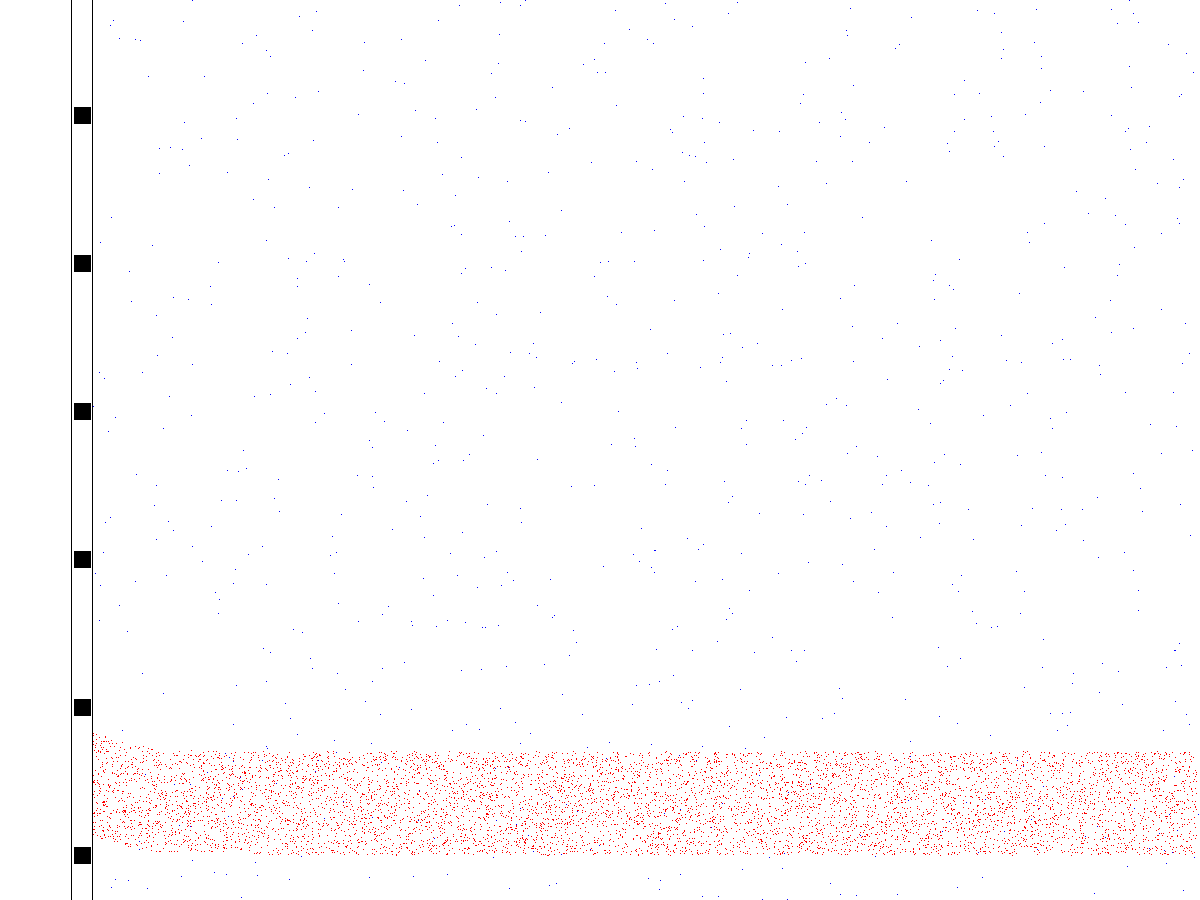
\includegraphics[width=50mm]{momentum_diffusion_particles4.png}}
    \put(55, 20){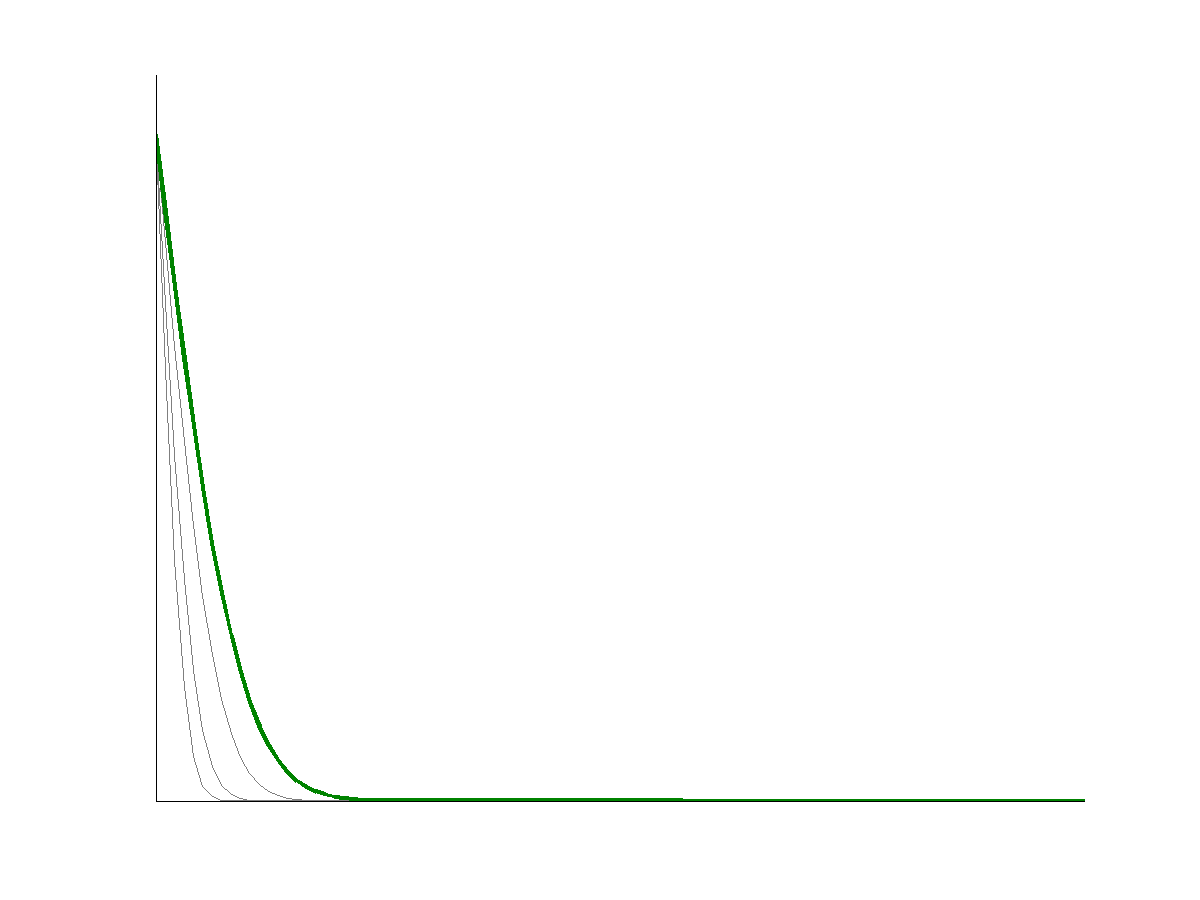
\includegraphics[width=45mm]{momentum_diffusion_profile4.png}}
    %\put(60.9, 51.2){\linethickness{0.01mm}\line(1, 0){34.9}}
    \put(59, 23){$0$}
    \put(97, 23){$x$}
    \put(57, 48){$U_1$}
    \put(83, 46){$u(y, t)$}
    \put(40, 40){$t=t_4$}
    \put( 4, 10){\color{vert} \line(1, 0){46}}
    \put(54, 10){\line(1, 0){10}}
    \put(64, 10){\vector(1, 1){10}}
    \put(73, 15){mesure du profil de}
    \put(72, 12){vitesse verticale $u(y, t)$}
    \put(1,0){\vector(0, 1){20}}
    \put(-1, 28){$U_1$}
    \put(0, 25){\rotatebox{90}{$=$}}
    \put(-2, 22){$Cte$}
    \put(61,25){\color{rouge} \vector(1, 0){4.5} \scriptsize $\delta(t_4)$}
    \put(4.5, 0){\color{rouge} \scriptsize $\delta(t_4)$}
    \end{picture}
  \end{center}

  \onslide<8>   
  \begin{center}
    \begin{picture}(100, 50)
    \put( 0, 0){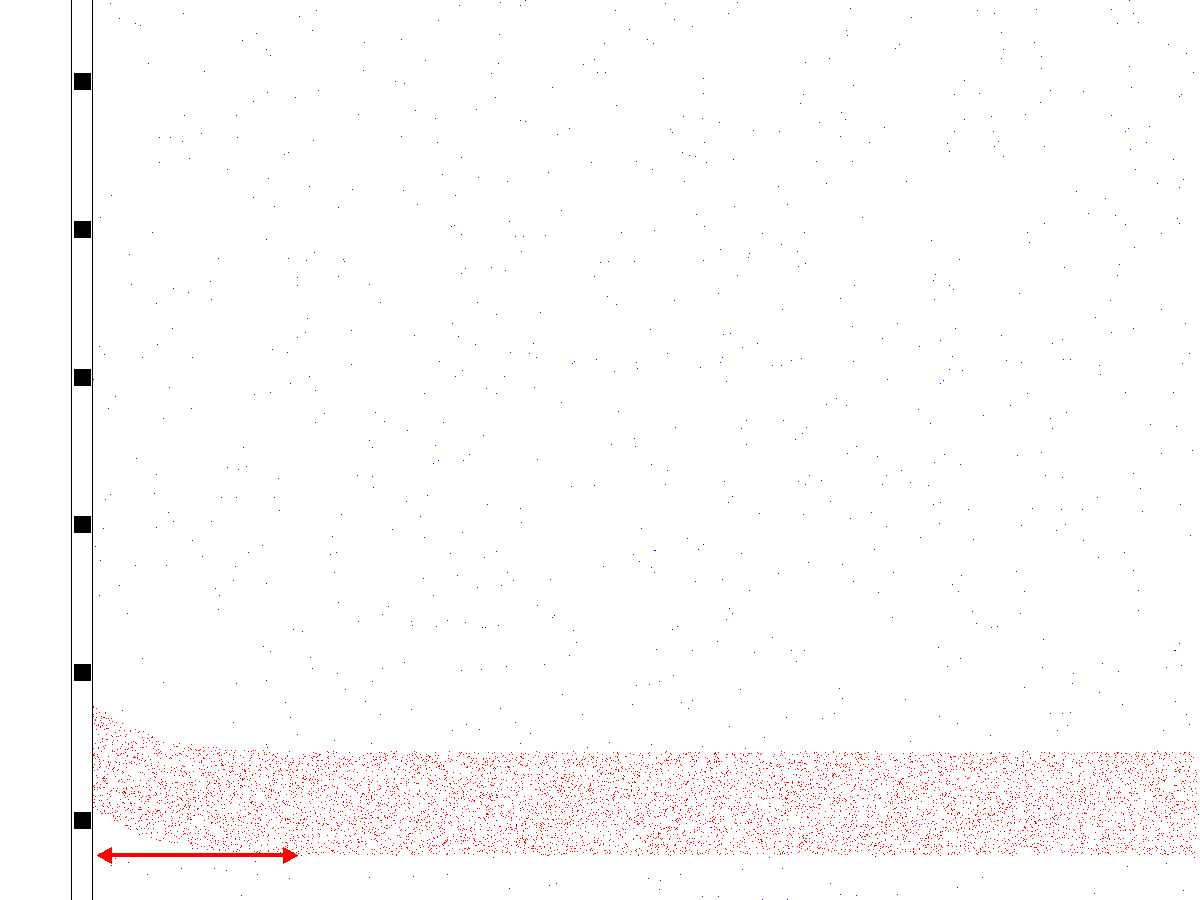
\includegraphics[width=50mm]{momentum_diffusion_particles5.png}}
    \put(55, 20){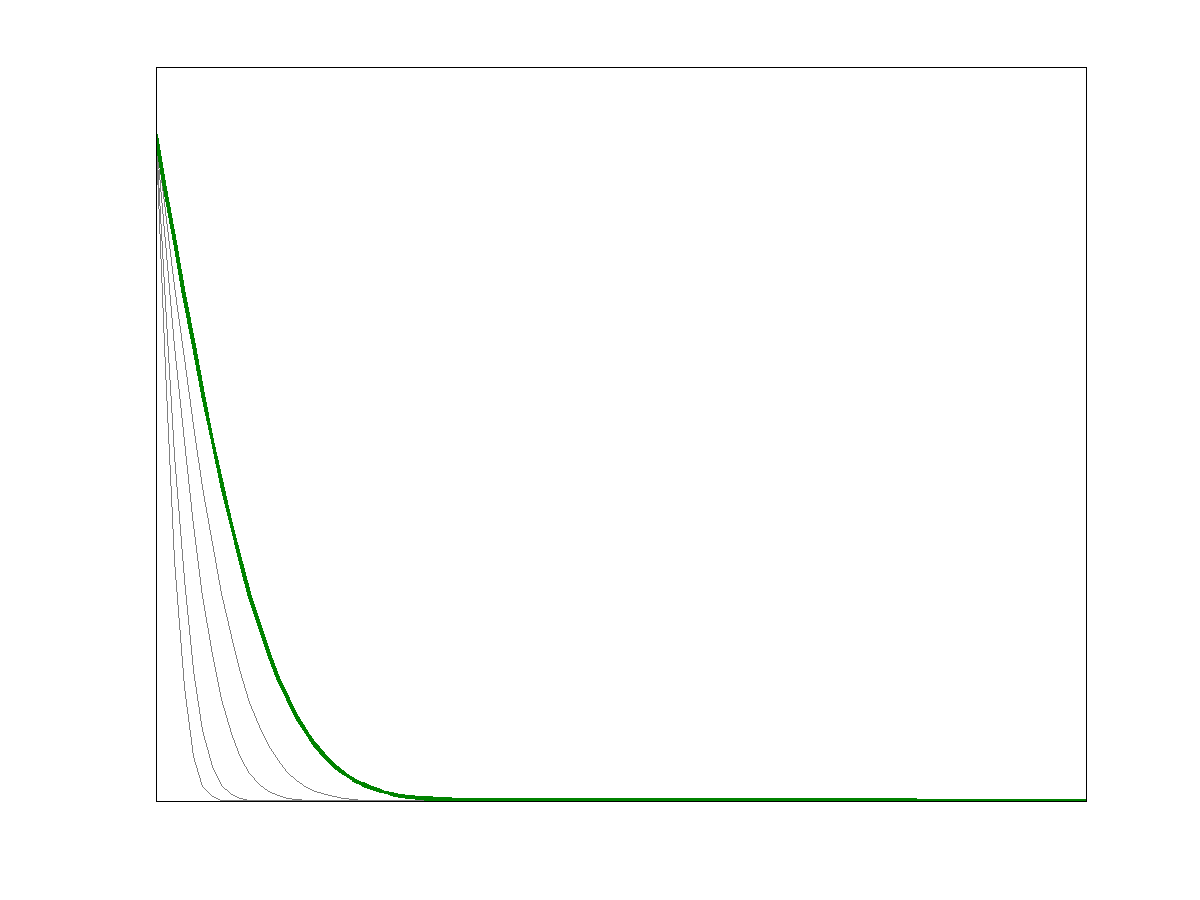
\includegraphics[width=45mm]{momentum_diffusion_profile5.png}}
    %\put(60.9, 51.2){\linethickness{0.01mm}\line(1, 0){34.9}}
    \put(59, 23){$0$}
    \put(97, 23){$x$}
    \put(57, 48){$U_1$}
    \put(83, 46){$u(y, t)$}
    \put(40, 40){$t=t_5$}
    \put( 4, 10){\color{vert} \line(1, 0){46}}
    \put(54, 10){\line(1, 0){10}}
    \put(64, 10){\vector(1, 1){10}}
    \put(73, 15){mesure du profil de}
    \put(72, 12){vitesse verticale $u(y, t)$}
    \put(1,0){\vector(0, 1){20}}
    \put(-1, 28){$U_1$}
    \put(0, 25){\rotatebox{90}{$=$}}
    \put(-2, 22){$Cte$}
    \put(61,25){\color{rouge} \vector(1, 0){6.5} \scriptsize $\delta(t_5)$}
    \put(5.5, 0){\color{rouge} \scriptsize $\delta(t_5)$}
    \end{picture}
  \end{center}

  \onslide<9>   
  \begin{center}
    \begin{picture}(100, 50)
    \put( 0, 0){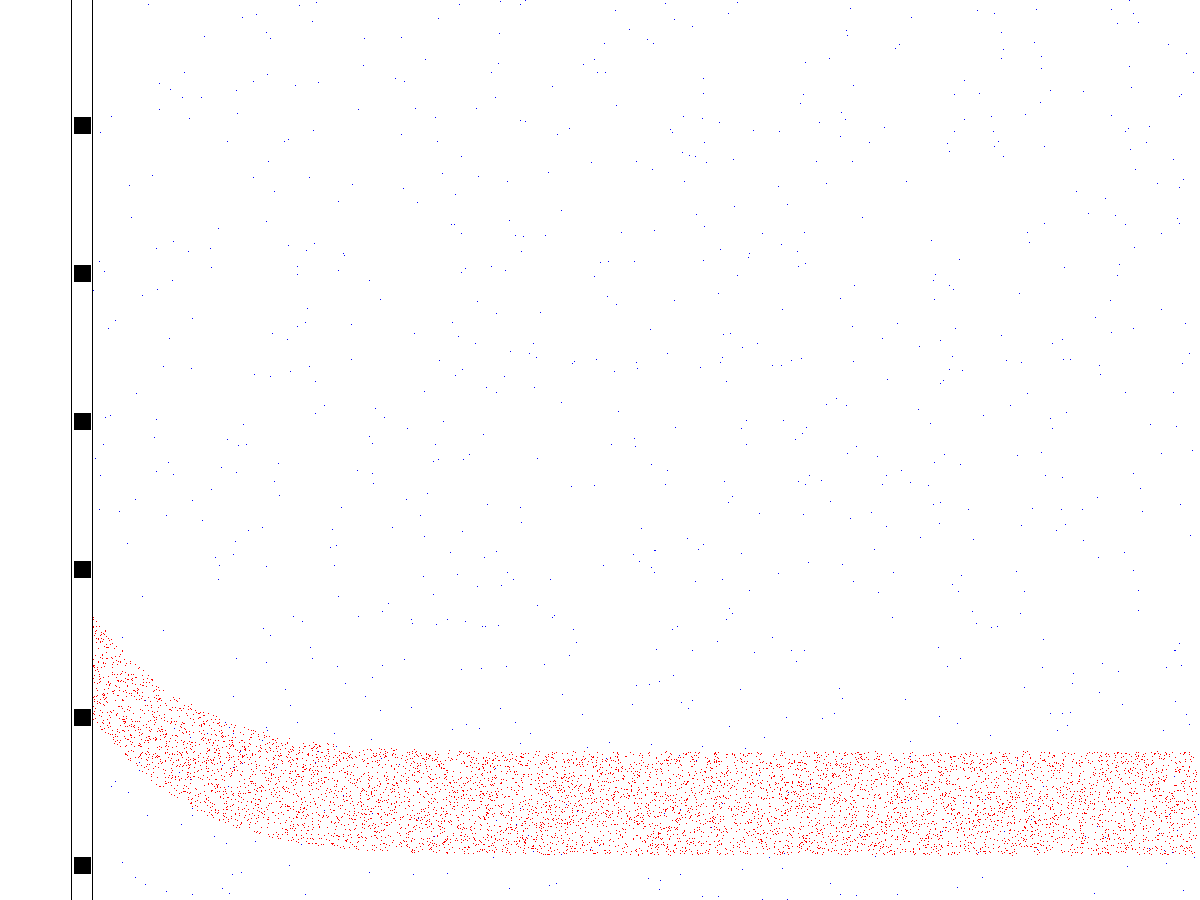
\includegraphics[width=50mm]{momentum_diffusion_particles6.png}}
    \put(55, 20){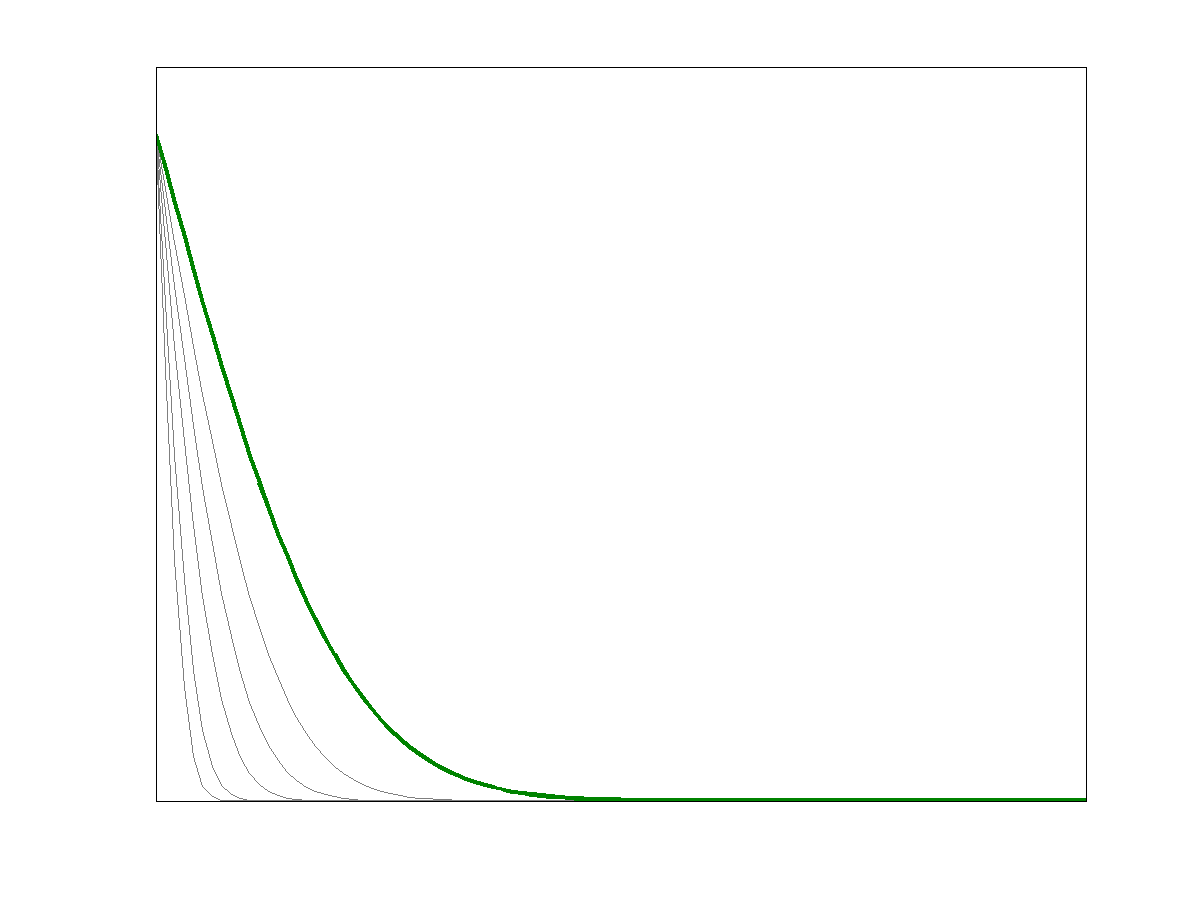
\includegraphics[width=45mm]{momentum_diffusion_profile6.png}}
    %\put(60.9, 51.2){\linethickness{0.01mm}\line(1, 0){34.9}}
    \put(59, 23){$0$}
    \put(97, 23){$x$}
    \put(57, 48){$U_1$}
    \put(83, 46){$u(y, t)$}
    \put(40, 40){$t=t_6$}
    \put( 4, 10){\color{vert} \line(1, 0){46}}
    \put(54, 10){\line(1, 0){10}}
    \put(64, 10){\vector(1, 1){10}}
    \put(73, 15){mesure du profil de}
    \put(72, 12){vitesse verticale $u(y, t)$}
    \put(1,0){\vector(0, 1){20}}
    \put(-1, 28){$U_1$}
    \put(0, 25){\rotatebox{90}{$=$}}
    \put(-2, 22){$Cte$}
    \put(61,25){\color{rouge} \vector(1, 0){10.5}}
    \put(72,25.5){\color{rouge} \scriptsize $\delta(t_6)$}
    \put(8, 0){\color{rouge} \scriptsize $\delta(t_6)$}
    \end{picture}
  \end{center}

  \onslide<10>   
  \begin{center}
    \begin{picture}(100, 50)
    \put( 0, 0){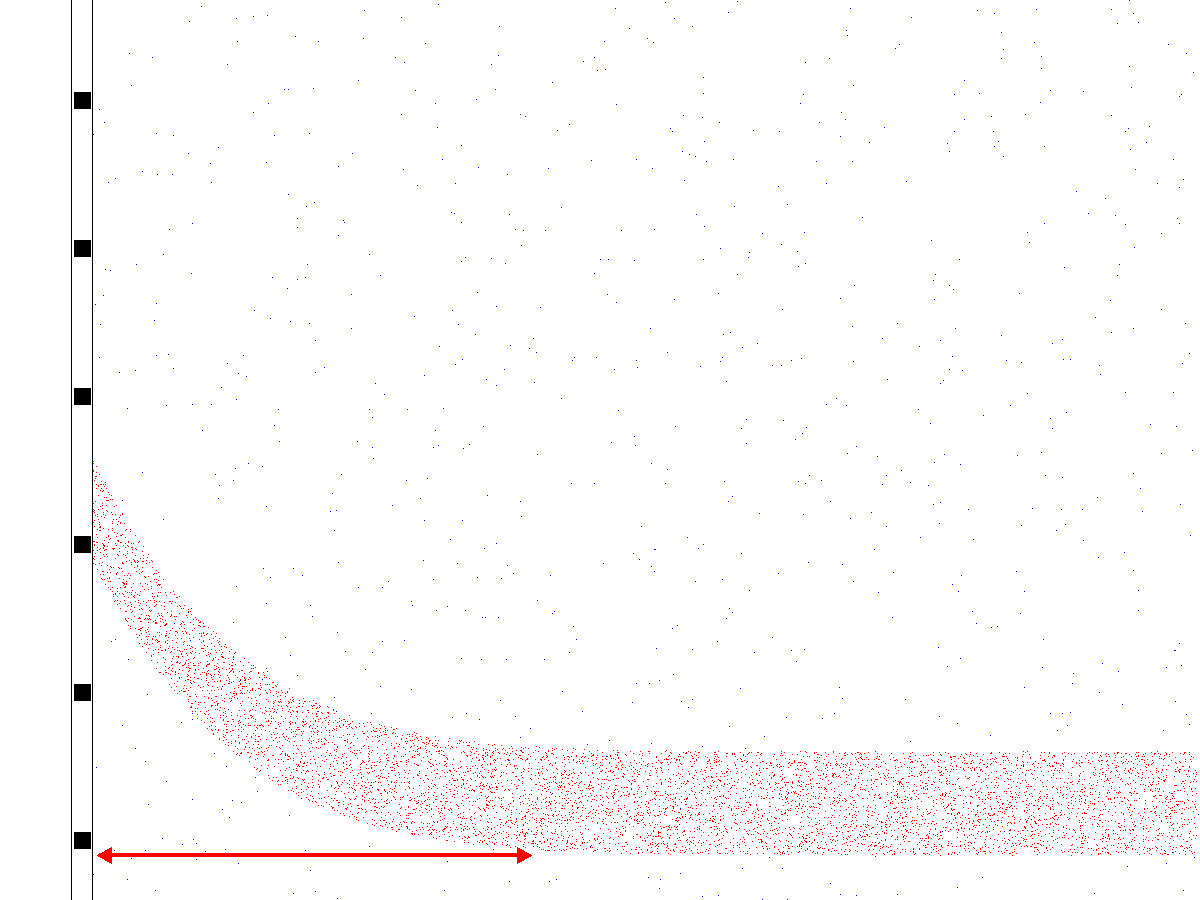
\includegraphics[width=50mm]{momentum_diffusion_particles7.png}}
    \put(55, 20){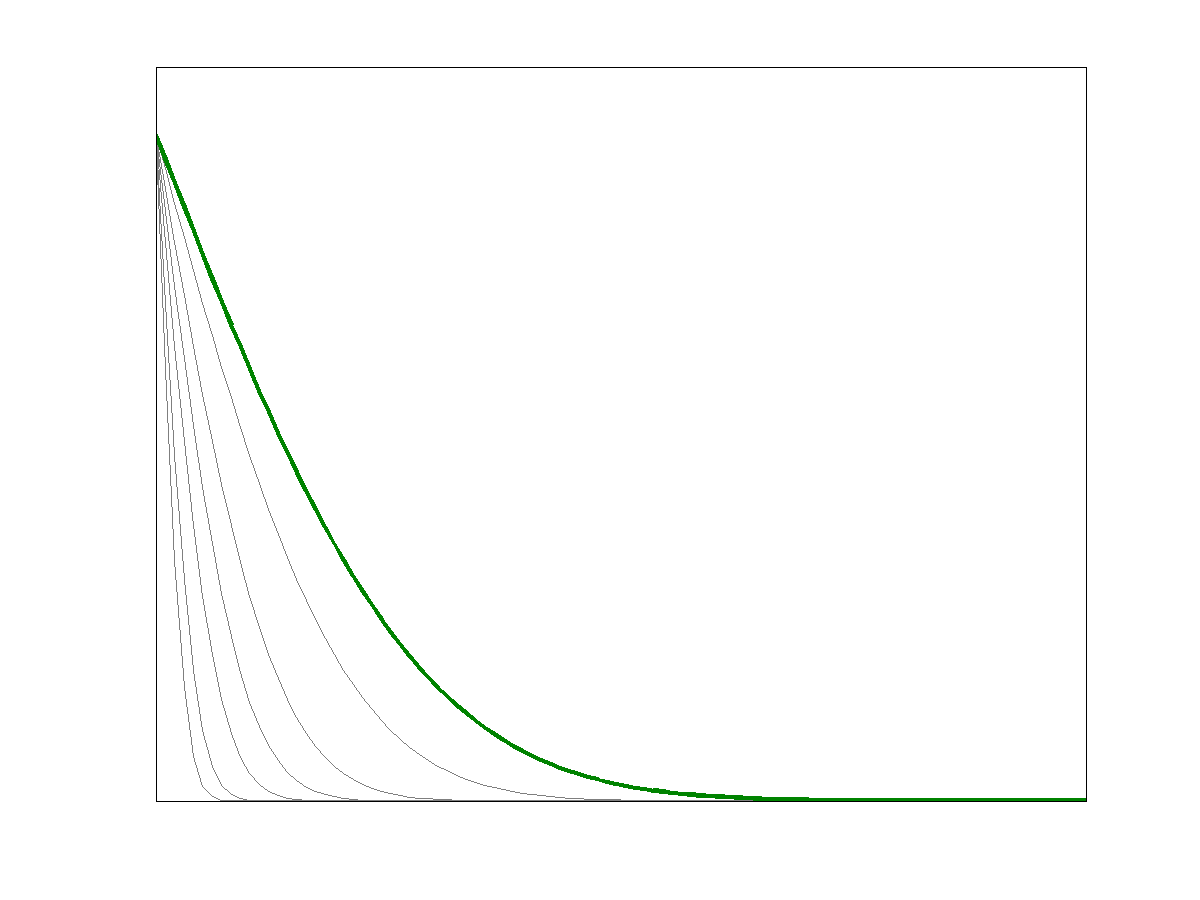
\includegraphics[width=45mm]{momentum_diffusion_profile7.png}}
    %\put(60.9, 51.2){\linethickness{0.01mm}\line(1, 0){34.9}}
    \put(59, 23){$0$}
    \put(97, 23){$x$}
    \put(57, 48){$U_1$}
    \put(83, 46){$u(y, t)$}
    \put(40, 40){$t=t_7$}
    \put( 4, 10){\color{vert} \line(1, 0){46}}
    \put(54, 10){\line(1, 0){10}}
    \put(64, 10){\vector(1, 1){10}}
    \put(73, 15){mesure du profil de}
    \put(72, 12){vitesse verticale $u(y, t)$}
    \put(1,0){\vector(0, 1){20}}
    \put(-1, 28){$U_1$}
    \put(0, 25){\rotatebox{90}{$=$}}
    \put(-2, 22){$Cte$}
    \put(61,25){\color{rouge} \vector(1, 0){14.5}}
    \put(76,25.7){\color{rouge} \scriptsize $\delta(t_7)$}
    \put(11, 0){\color{rouge} \scriptsize $\delta(t_7)$}
    \end{picture}
  \end{center}

  \onslide<11>   
  \begin{center}
    \begin{picture}(100, 50)
    \put( 0, 0){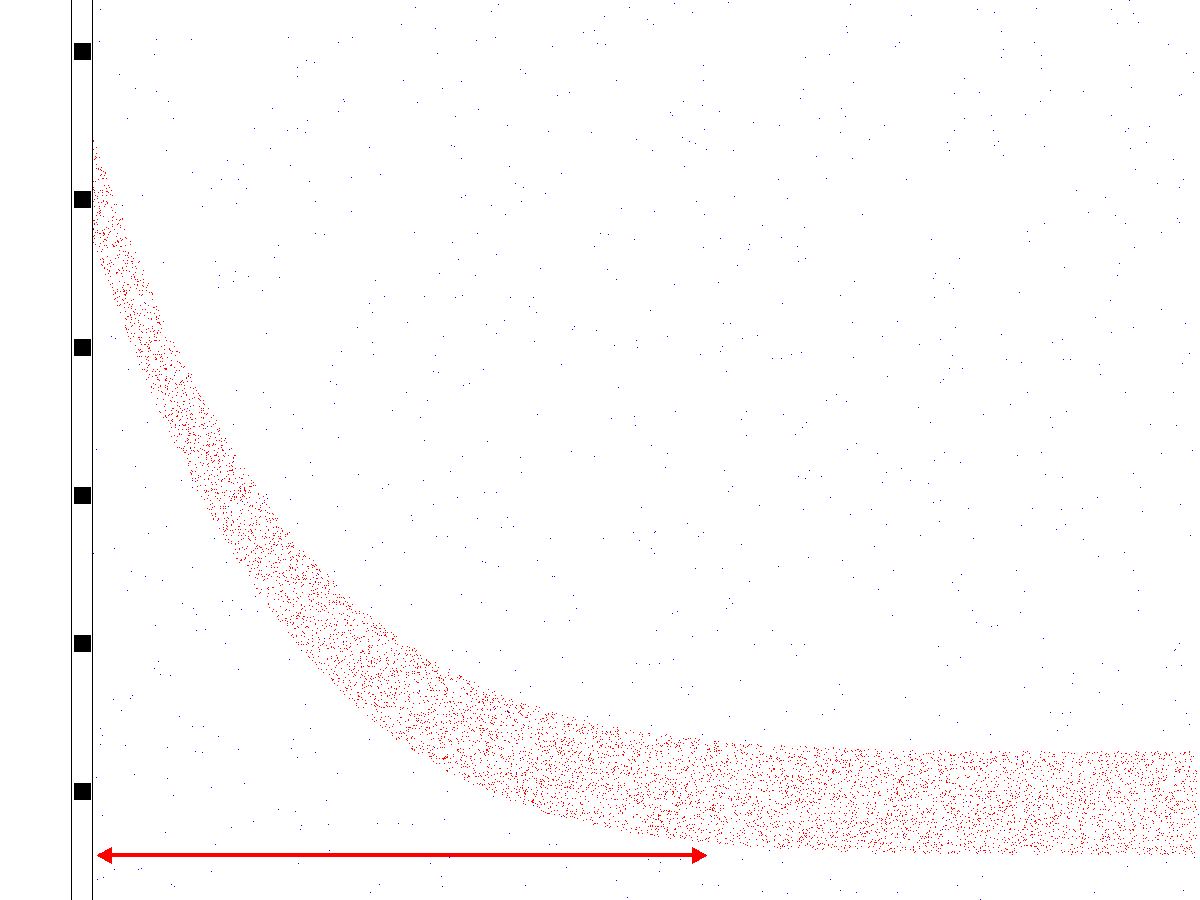
\includegraphics[width=50mm]{momentum_diffusion_particles8.png}}
    \put(55, 20){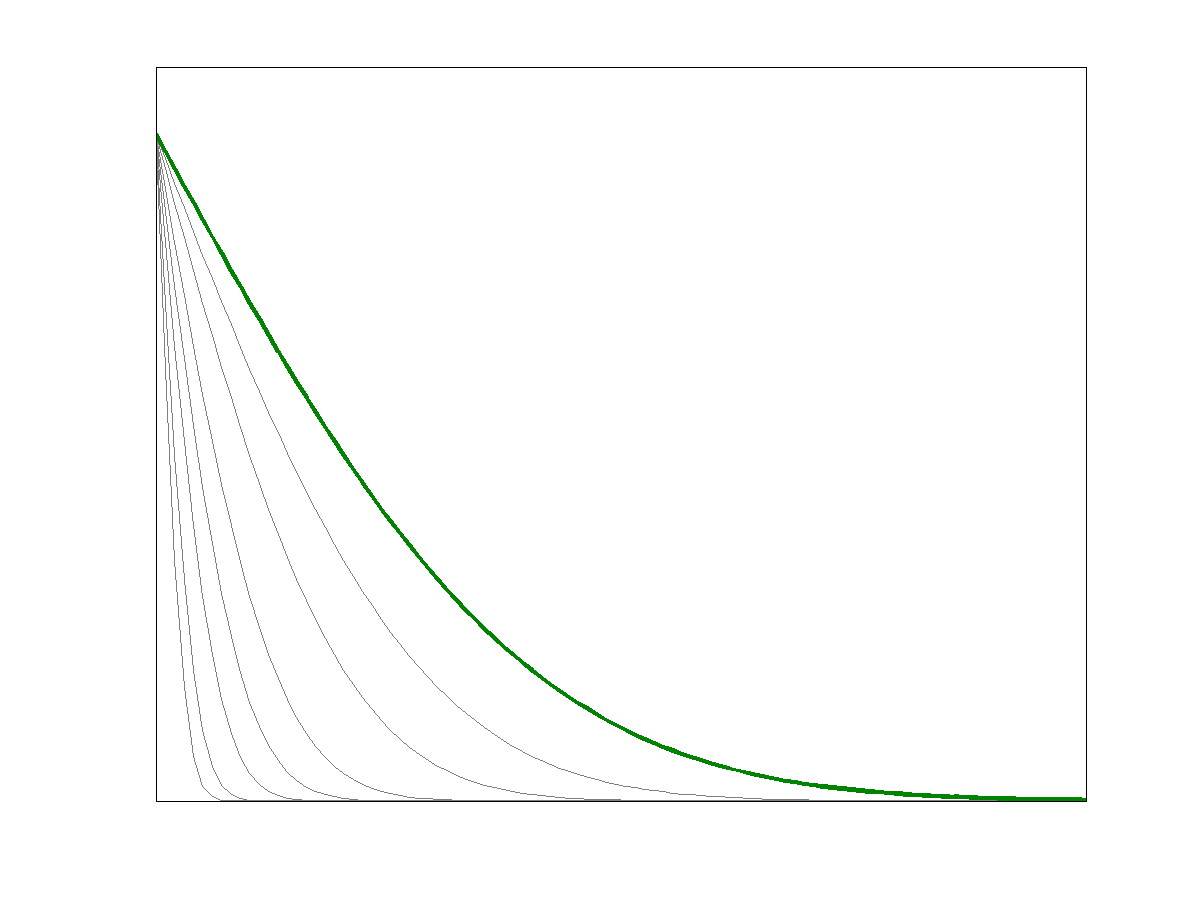
\includegraphics[width=45mm]{momentum_diffusion_profile8.png}}
    %\put(60.9, 51.2){\linethickness{0.01mm}\line(1, 0){34.9}}
    \put(59, 23){$0$}
    \put(97, 23){$x$}
    \put(57, 48){$U_1$}
    \put(83, 46){$u(y, t)$}
    \put(40, 40){$t=t_8$}
    \put( 4, 10){\color{vert} \line(1, 0){46}}
    \put(54, 10){\line(1, 0){10}}
    \put(64, 10){\vector(1, 1){10}}
    \put(73, 15){mesure du profil de}
    \put(72, 12){vitesse verticale $u(y, t)$}
    \put(1,0){\vector(0, 1){20}}
    \put(-1, 28){$U_1$}
    \put(0, 25){\rotatebox{90}{$=$}}
    \put(-2, 22){$Cte$}
    \put(61,25){\color{rouge} \vector(1, 0){20.5}}
    \put(81.5,25.8){\color{rouge} \scriptsize $\delta(t_8)$}
    \put(15, 0){\color{rouge} \scriptsize $\delta(t_8)$}
    \end{picture}
  \end{center}

  \onslide<12>   
  \begin{center}
    \begin{picture}(100, 50)
    \put( 0, 0){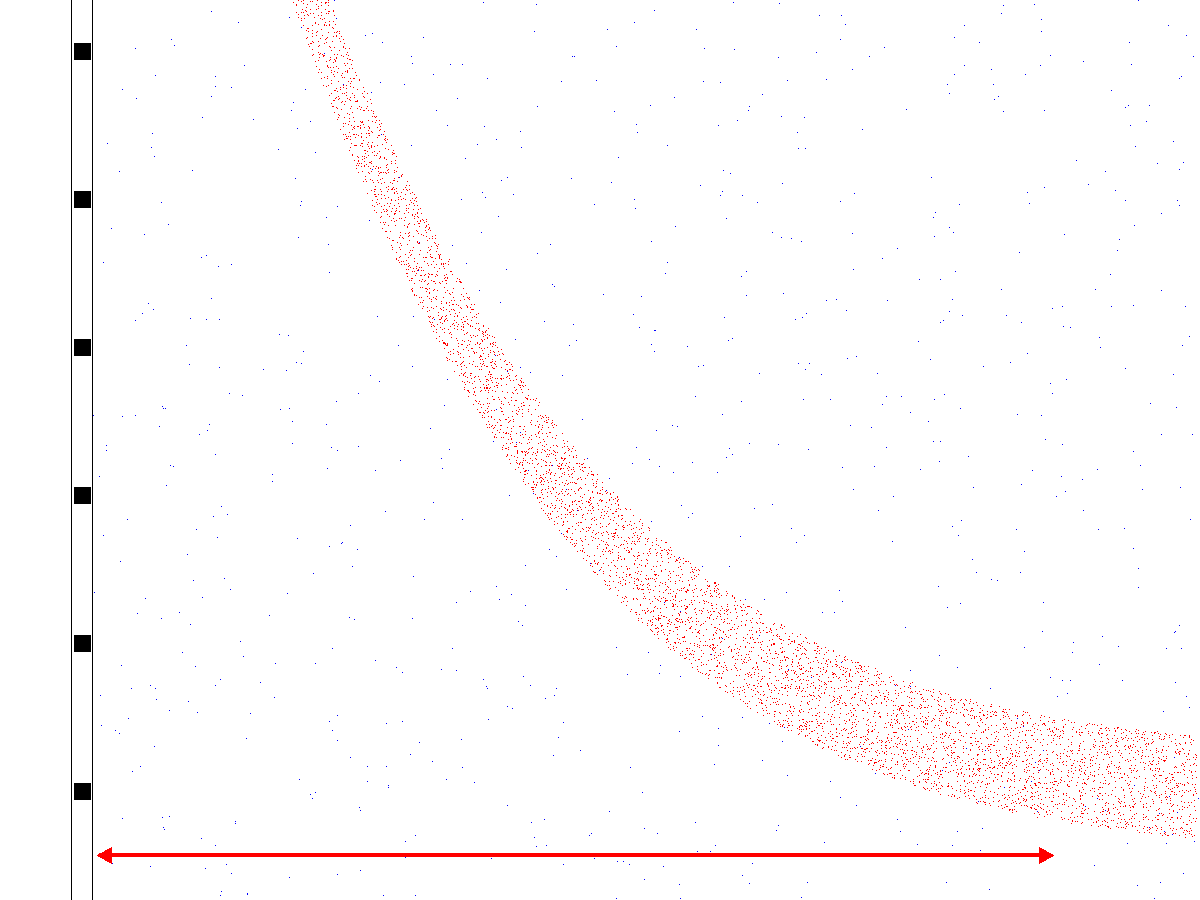
\includegraphics[width=50mm]{momentum_diffusion_particles9.png}}
    \put(55, 20){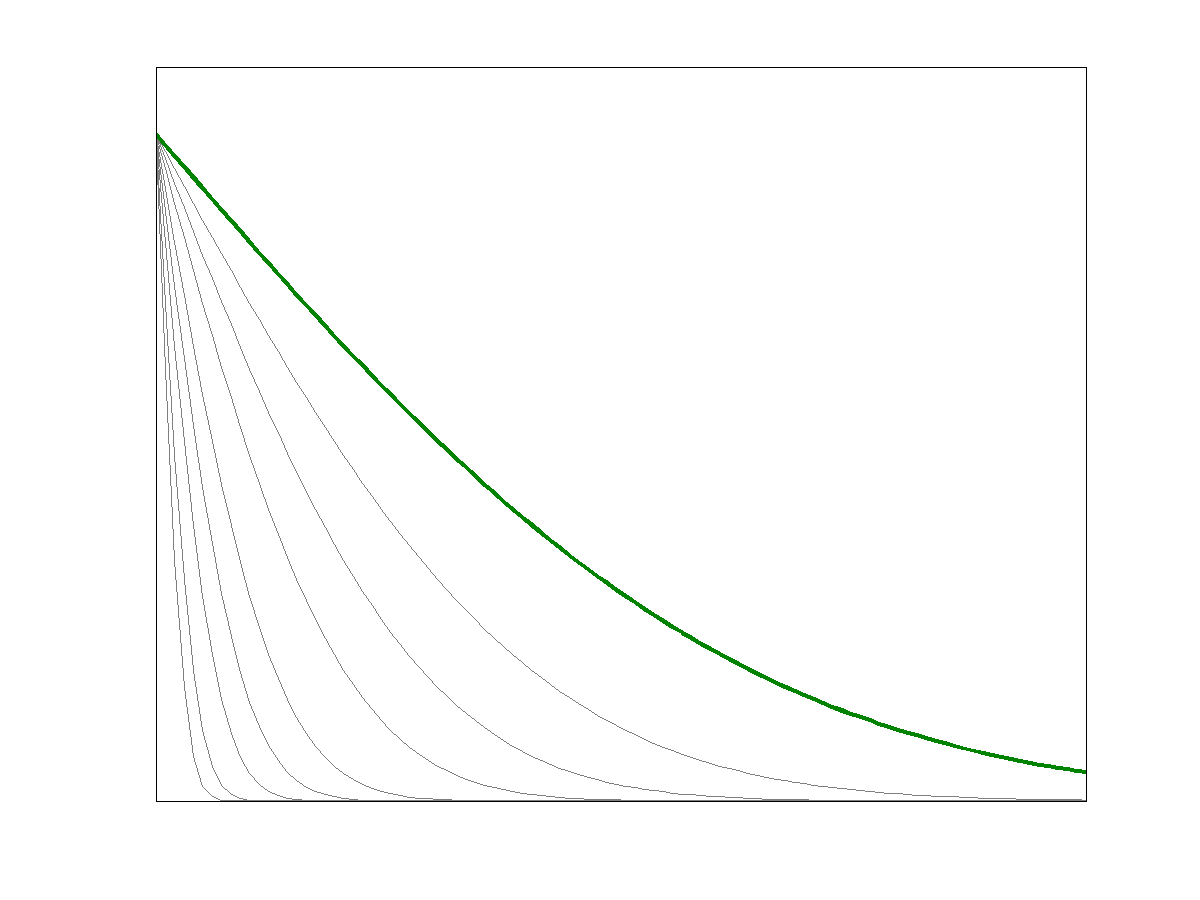
\includegraphics[width=45mm]{momentum_diffusion_profile9.png}}
    %\put(60.9, 51.2){\linethickness{0.01mm}\line(1, 0){34.9}}
    \put(59, 23){$0$}
    \put(97, 23){$x$}
    \put(57, 48){$U_1$}
    \put(83, 46){$u(y, t)$}
    \put(40, 40){$t=t_9$}
    \put( 4, 10){\color{vert} \line(1, 0){46}}
    \put(54, 10){\line(1, 0){10}}
    \put(64, 10){\vector(1, 1){10}}
    \put(73, 15){mesure du profil de}
    \put(72, 12){vitesse verticale $u(y, t)$}
    \put(1,0){\vector(0, 1){20}}
    \put(61,25){\color{rouge} \vector(1, 0){32.5}}
    \put(90,27){\color{rouge} \scriptsize $\delta(t_9)$}
    \put(20, 0){\color{rouge} \scriptsize $\delta(t_9)$}
    \put(-1, 28){$U_1$}
    \put(0, 25){\rotatebox{90}{$=$}}
    \put(-2, 22){$Cte$}
    \end{picture}
  \end{center}

  \onslide<13>   
  \begin{center}
    \begin{picture}(100, 50)
    \put( 0, 0){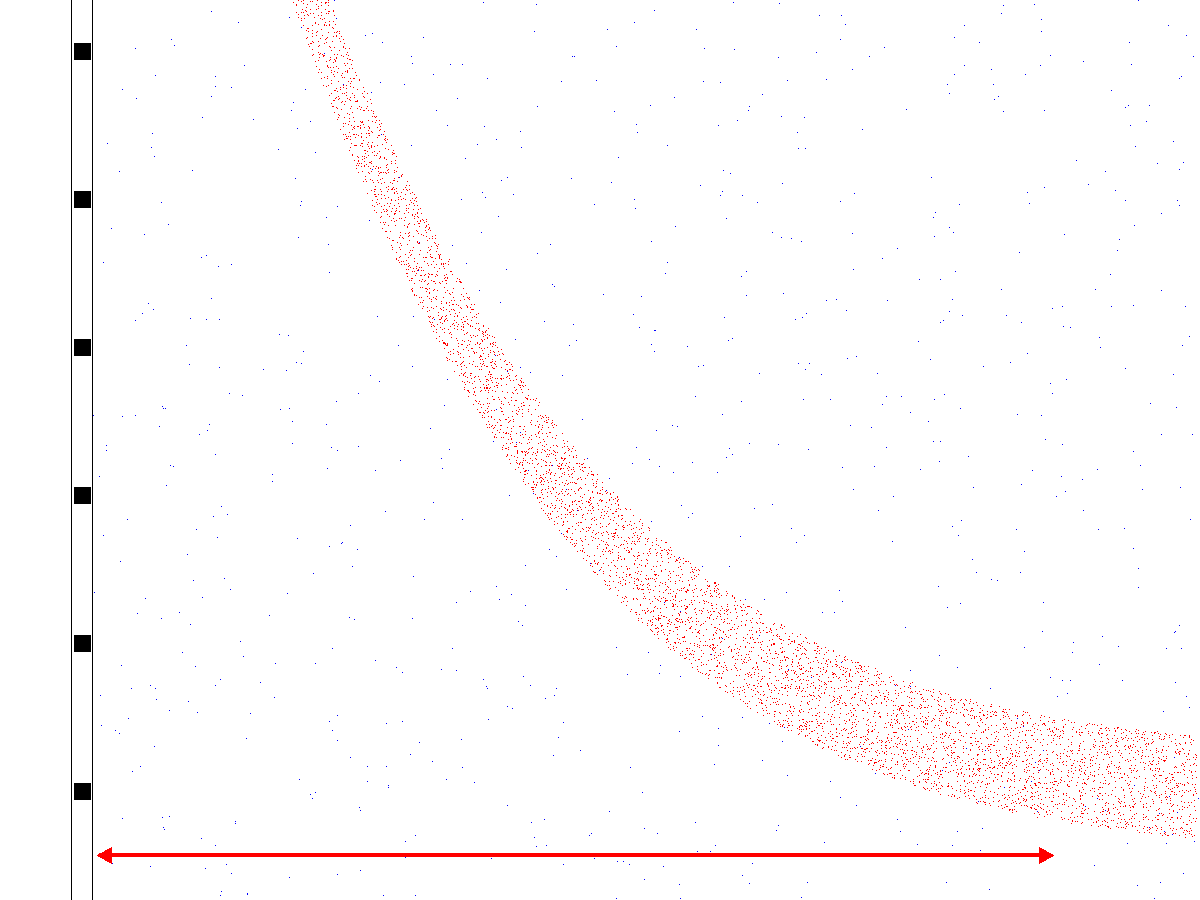
\includegraphics[width=50mm]{momentum_diffusion_particles9.png}}
    \put(55, 20){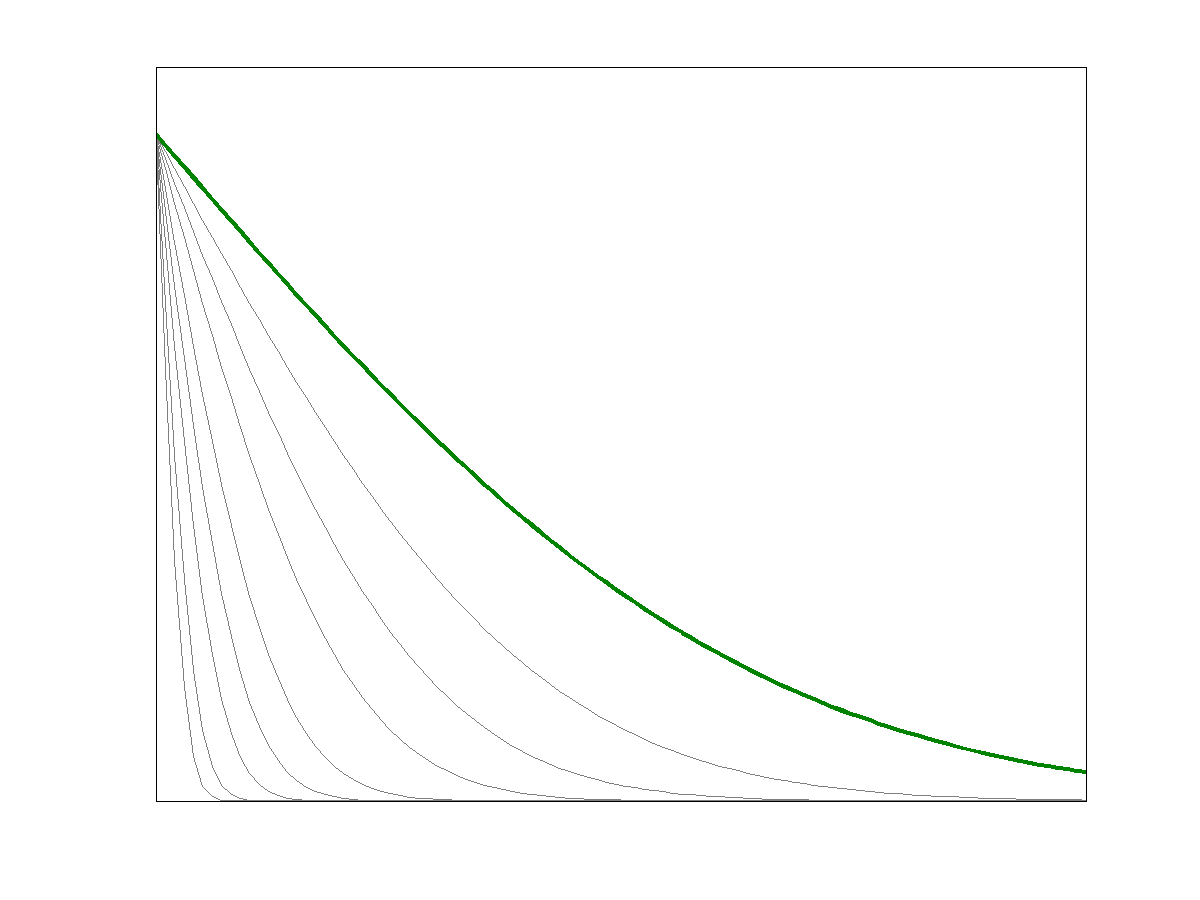
\includegraphics[width=45mm]{momentum_diffusion_profile9.png}}
    %\put(60.9, 51.2){\linethickness{0.01mm}\line(1, 0){34.9}}
    \put(59, 23){$0$}
    \put(97, 23){$x$}
    \put(57, 48){$U_1$}
    \put(83, 46){\color{rouge}$u(y, t)$}
%    \put(40, 40){$t=t_9$}
    \put( 4, 10){\color{vert} \line(1, 0){46}}
    \put(54, 10){\line(1, 0){10}}
    \put(64, 10){\vector(1, 1){10}}
    \put(73, 15){mesure du profil de}
    \put(72, 12){vitesse verticale $u(y, t)$}
    \put(1,0){\vector(0, 1){20}}
    \put(-1, 28){$U_1$}
    \put(0, 25){\rotatebox{90}{$=$}}
    \put(-2, 22){$Cte$}
    \put(61,25){\color{rouge} \vector(1, 0){32.5}}
    \put(90,27){\color{rouge} $\delta(t)$}
    \put(20, -1){\color{rouge}$\delta(t)$}
    \end{picture}
  \end{center}

\bigskip

  \hfill $\rightarrow$ Objectifs : déterminer l'évolution du profil de vitesse verticale \textcolor{rouge}{$u(y, t)$} 
  et la loi de diffusion \textcolor{rouge}{$\delta(t)$}

\end{overprint}

\vspace{0mm}

\end{frame}


\begin{frame}{Etude Mathématique}
\small

\begin{itemize}
\item {\bf Solution exacte :}  cf. TD, exercice 4.0 (correction sur moodle).

\item Etude par analyse dimensionnelle

Cherchons à estimer $\delta(t)$ par analyse dimensionnelle (méthode du chapitre 1):

- Recherche des paramètres pertinents : 
$$
\delta = {\cal F} ( t, \nu, \rho, U) 
$$
- Simplification issue de l'étude de la structure des équations : le problème est {\em linéaire} et la solution adimensionnelle $\bar{u} = u(y,t)/U$ ne dépend pas 
de $U$ !

- Finalement on peut partir d'une relation de la forme :
$$
\delta = {\cal F} ( t, \nu, \rho) 
$$


Méthode du chapitre 1 : mise sous forme adimensionnelle avec $[T] = t, [L]  = \sqrt{\nu t}$ (seule échelle de longueur du problème), $[M] = \rho [L]^{3/2}$.


$=>$ $\delta = \sqrt{\nu t} \times C_{te}$
 

(Remarque : méthode plus générale, identification du {\em groupe de symétries} du problème ; cf. correction moodle).
\end{itemize}

$\delta(t) = \sqrt{\nu t}$ est appelée la {\em longueur de pénétration visqueuse} On retrouve cette échelle de longueur dans de nombreux problèmes instationnaires apparentés !

\end{frame}


\begin{frame}{1er problème de Stokes : Remarques}

\small
\bigskip
Envisageons le problème d'une autre manière en posant la question différemment.

\pause
\medskip

{\bf Question :} A une distance $y=L$ de la paroi, a partir de quel instant $t$ le fluide se met-il en mouvement ?
\pause
\medskip

Réponse par analyse dimensionnelle :
 
$$t = {\cal F} ( L,\nu,\rho, \cancel{U} )$$  

$$\rightarrow \qquad t_v = L^2/\nu \times C_{te}$$

\pause
\medskip

La quantité $\tau_\nu = L^2/ \nu $ est appelée le temps caractéristique de diffusion visqueuse. 

On retrouve cette échelle de longueur dans de nombreux problèmes instationnaires apparentés !



\end{frame}


\begin{frame}{Second problème de Stokes}

{\bf Problème :} Ecoulement instationnaire établi engendré par une paroi oscillante $U(y=0) = U cos (\omega t)$.

%\begin{picture}(0,0)%
%\epsfig{file=stokes-2.pstex}%
%\end{picture}%
%\setlength{\unitlength}{3108sp}%
%%
%\begingroup\makeatletter\ifx\SetFigFont\undefined%
%\gdef\SetFigFont#1#2#3#4#5{%
%  \reset@font\fontsize{#1}{#2pt}%
%  \fontfamily{#3}\fontseries{#4}\fontshape{#5}%
%  \selectfont}%
%\fi\endgroup%
%\begin{picture}(2397,1299)(221,-1031)
%\put(2296,-331){\makebox(0,0)[lb]{\smash{\SetFigFont{8}{9.6}{\familydefault}{\mddefault}{\updefault}$\vec{e}_y$}}}
%\put(2491,-576){\makebox(0,0)[lb]{\smash{\SetFigFont{8}{9.6}{\familydefault}{\mddefault}{\updefault}$\vec{e}_x$}}}
%\put(687,-854){\makebox(0,0)[lb]{\smash{\SetFigFont{6}{7.2}{\familydefault}{\mddefault}{\updefault}$U\cos(\omega t)$}}}
%\end{picture}

\bigskip

\begin{itemize}

\item Etude par analyse dimensionnelle :

Estimons l'épaisseur caractéristique $\delta$ du fluide mis en mouvement :

$$
\delta = {\cal F} ( \omega, \nu, \rho, \cancel{U}) 
$$



$=>$ $\delta = \sqrt{\nu / \omega} \times C_{te}$


\item {\bf Solution exacte :}  cf. TD, exercice 4.1 

$$
u(y,t) = U e^{-y/\delta} \cos (\omega t - y/\delta) \quad \mbox{ avec } \delta = \sqrt{\frac{2 \nu }{\omega}}
$$

\end{itemize}

\end{frame}



 
 \begin{frame}{ Ecoulement pulsé en conduite (1) }

\small

Etudions l'écoulement  d'un fluide soumis à un gradient de pression périodique,

 dans un canal horizontal ($g_x = 0$) d'épaisseur $h$ :
 
 
$ \frac{1}{\rho} \frac{\partial p }{\partial x} = K \cos (\omega t)$

$$ 
\frac{\partial u}{\partial t} = - K cos(\omega t) + \nu \frac{\partial^2 u}{\partial y^2 }
$$

\pause 
\smallskip
Cherchons à simplifier le problème par {\em analyse dimensionnelle des équations} :

Posons $U$ = échelle  caractéristique (ou jauge)  de vitesse. 

L'échelle de temps est $T = \omega^{-1}$, et l'échelle de longueur est (a priori) $h$.


$$ 
\begin{array}{lccccc} 
\mbox{(equation :)} &
\frac{\partial u}{\partial t}  &= & - K cos(\omega t) &+ & \nu \frac{\partial^2 u}{\partial y^2} \\
\mbox{(terme :)} &
\left[I\right] && \left[P\right] &&\left[V\right] \\
\mbox{(Ordre de grandeur :)} &
\frac{U}{T}  && K && \nu \frac{U}{h^2}
\end{array}
$$

Le terme $[P]$ est nécessairement présent à l'ordre dominant. Comparons les termes  $[V] $ et $[I]$ :

$$ 
\frac{[I]}{[V]} =  \frac{h^2 \omega}{\nu} = St 
$$

Ceci définit le Nombre de Stokes de l'écoulement. 

\end{frame}

 \begin{frame}{ Ecoulement pulsé en conduite (2) }

\small

\begin{itemize}
\item Si $St \ll 1$ alors $[I] \ll [V]$, a l'ordre dominant on peut négliger $[I]$ et ne garder que $[V]$ et $[P]$.
$$ 
0 = - K cos(\omega t) + \nu \frac{\partial^2 u}{\partial y^2 }
$$

$=>$ Solution : $u(y,t) \approx - K \cos (\omega t) \left( 1 - y^2/h^2 \right) $ "ecoulement de Poiseuille quasi-statique".

\medskip 

\item  
Si $St \gg 1$ alors $[V] \gg [I]$, a l'ordre dominant on peut négliger $[V]$ et ne garder que $[I]$ et $[P]$.
$$ 
\frac{\partial u}{\partial t}  = - K cos(\omega t) 
$$

$=>$ Solution : $u(y,t) \approx - \frac{K}{\omega} \sin \omega t$

Remarque : cette solution ne vérifie pas la condition limite d'adhérence... en réalité il se forme une "couche limite de Stokes" d'épaisseur $\delta$ (cf. problème précédent). 
 
 \medskip

\item 
Si $St = {\cal  O}(1)$, pas de simplification possible, il faut garder $[V]$ et $[I]$.

$=>$ Solution possible par voie analytique mais compliquée... (cf. TP numérique).

\end{itemize}

 
 \end{frame}



%\pause
%\medskip


\begin{frame}{Remarques Complémentaires}

\small

\begin{enumerate}

\item 
En dérivant l'équation des films plans par rapport à $y$ et en notant que $\omega_z =  \cancel{\frac{\partial v}{\partial x}} -  \frac{\partial u}{\partial y}$ ,
on peut montrer que la vorticité est elle-aussi gouvernée par une équation de diffusion:

$$
\frac{\partial \omega_z}{\partial t} = \nu \frac{\partial^2 \omega_z}{\partial y^2} 
$$ 

La viscosité peut donc également être interprétée comme un {\em mécanisme de diffusion de la vorticité}.

\item On note qu'il n'y a {\em pas de terme source} dans cette équation. Le seul terme de production de vorticité vient de la condition limite sur une 
paroi. En effet la vorticité est directement reliée à la contrainte visqueuse exercée sur un paroi : $\tau_{xy} = (- \mu /2) \omega_z $

{\bf Conséquence :} Dans un écoulement plan parallèle de la vorticité est créée par le frottement sur les parois, puis diffuse dans le volume
(on généralisera ce résultat au chapitre 8).

%\item On peut noter par ailleurs que la vorticité est directement reliée à la contrainte visqueuse :

%En effet pour les écoulements plans parallèles 
%$$ \omega_z(y= = \cancel{\frac{\partial v}{\partial x}} -  \frac{\partial u}{\partial y} ; \qquad 
%\tau_{xy} = \frac{\mu}{2} \left( \cancel{\frac{\partial v}{\partial x}} +  \frac{\partial u}{\partial y} \right) ; \qquad \mbox{ donc } \tau_{xy} = - \mu \omega_z /2 
%$$


\item Il existe enfin une analogie entre la {\em diffusion de quantité de mouvement} (viscosité) et la diffusion de la chaleur (conduction thermique).
en effet les équations ont la même forme !

\smallskip
Equation de la conduction thermique 1D ($\theta = \theta(x,t)$) (cf. cours de transferts thermiques) :
$$
\frac{\partial \theta}{\partial t} = \frac{\sigma}{\rho c_p}  + \kappa \frac{\partial^2 \theta}{\partial x^2} 
$$ 

$\kappa = \frac{\lambda}{\rho c_p}$ Diffusivité thermique, même dimension physique que $\nu$ ! ( $[\kappa] = L^2 T^{-1}$).



\end{itemize}




\end{frame}


\comment{
%--------------------------------------------------------------------------------------------------
\begin{frame}{Constat :}
%--------------------------------------------------------------------------------------------------

\small

\begin{center}
  \begin{picture}(110, 30)
    \put(  0, 0){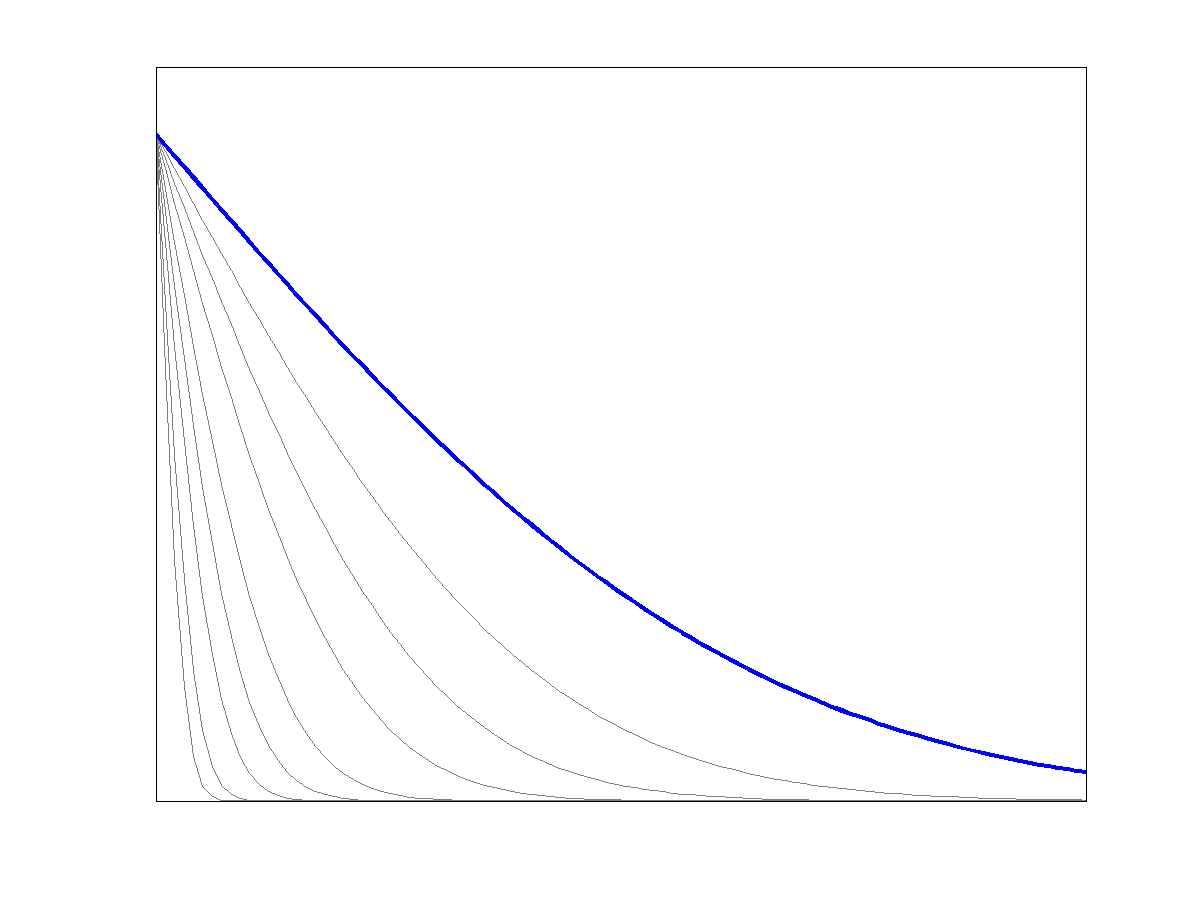
\includegraphics[width=35mm]{mass_diffusion_profile9.png}}
%    \put( 5, 5){\vector(1, 1){10}}
    \put( 4.5, 4){\color{bleu} \vector(1, 0){24}}
    \put( 27, 5.5){\color{bleu} \footnotesize $\delta(t)$}
%    \put(16, 16){$t$}
    \put(16, 0.5){$x$}
    \put(1, 22){$n_{i,1}$}
    \put(1, 2){$C_0$}
    \put(20, 20){\color{bleu}$n_i(x,t)$}
    \put( 37, 0){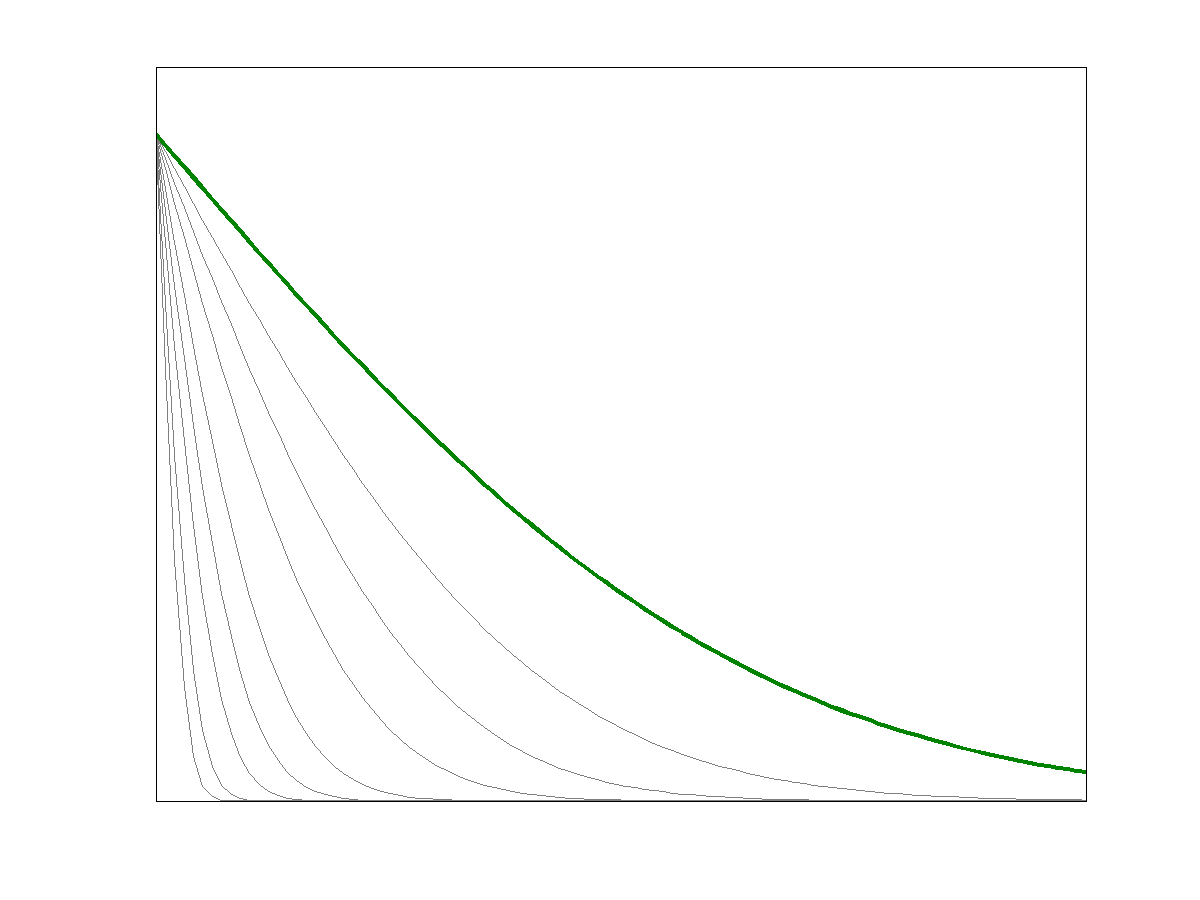
\includegraphics[width=35mm]{momentum_diffusion_profile9.png}}
%    \put(42, 10){\color{gris} \vector(1, 0){15}}
    \put(41.5, 4){\color{vert} \vector(1, 0){24}}
    \put(64, 5.5){\color{vert} \footnotesize $\delta(t)$}
%    \put(53, 16){$t$}
    \put(53, 0.5){$x$}
    \put(38, 22){$U_1$}
    \put(38, 2){$U_0$}
    \put(57, 20){\color{vert}$u(y, t)$}
    \put( 74, 0){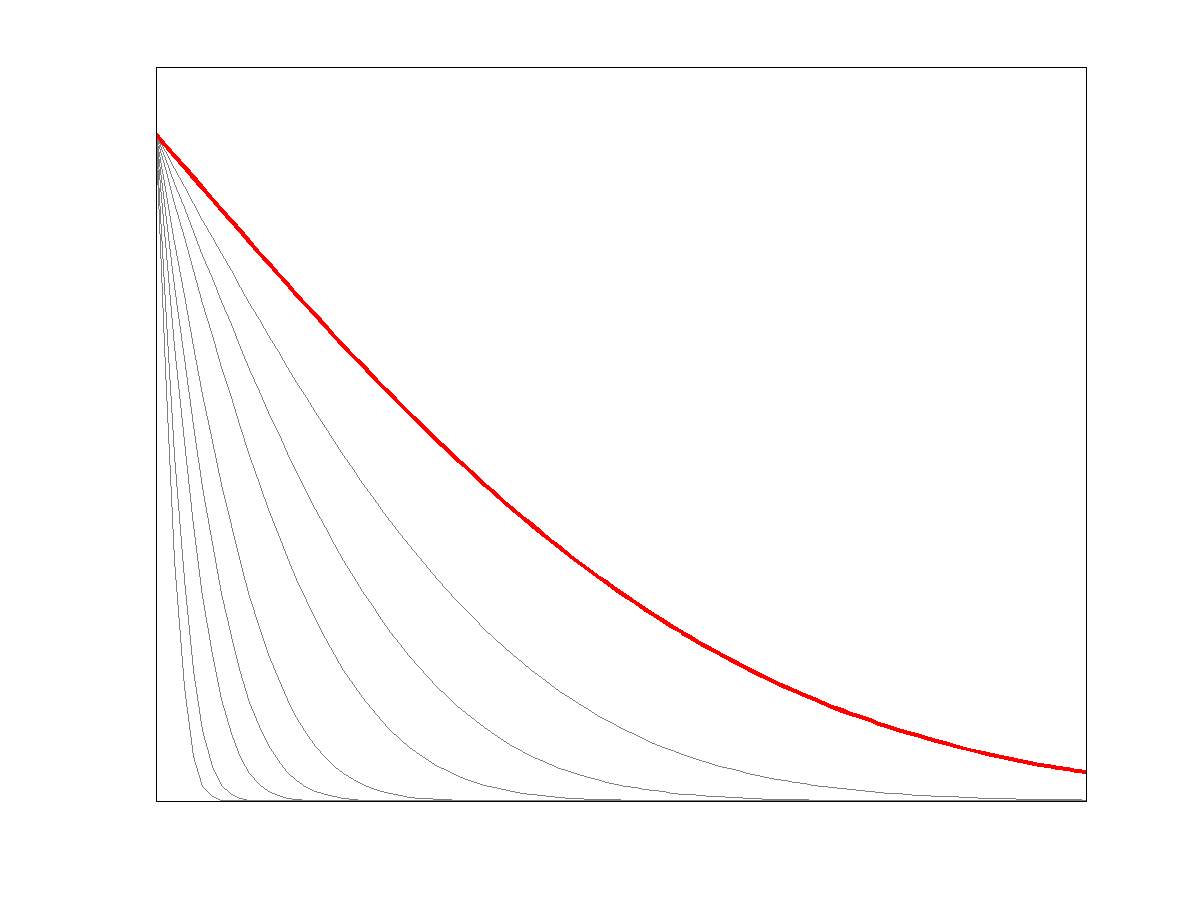
\includegraphics[width=35mm]{heat_diffusion_profile9.png}}
%    \put(79, 5){\vector(1, 1){10}}
    \put(78.5, 4){\color{rouge} \vector(1, 0){24}}
    \put(101, 5.5){\color{rouge} \footnotesize $\delta(t)$}
%    \put(90, 16){$t$}
    \put(90, 0.5){$x$}
    \put(75, 22){$T_1$}
    \put(75, 2){$T_0$}
    \put(94, 20){\color{rouge}$T(x, t)$}
  \end{picture}
\end{center}

\bigskip

On observe un phénomène \textcolor{rouge}{analogue} dans ces trois expériences : 

\medskip

\textbf{transport} de la quantité physique par l'agitation moléculaire 
depuis la paroi $x=0$ vers $x>0$,

sur une distance, appelée profondeur ou \textcolor{vert}{longueur de pénétration} $\delta(t)$
qui augmente avec le temps selon une loi commune, universelle, dite de diffusion, dont la prédiction théorique
est dérivée ci-après dans chaque cas.

\vspace{20mm}

\end{frame}

%--------------------------------------------------------------------------------------------------
\subsubsection{Diffusion de masse}

\begin{frame}{Diffusion de masse}
%--------------------------------------------------------------------------------------------------

\small

\textbf{Objectif :} 

\medskip

dériver l'\textcolor{rouge}{équation d'évolution} associée à la migration dans la direction $x$
d'une espèce $i$ dans un milieu au repos.

\vspace{50mm}

\end{frame}

%--------------------------------------------------------------------------------------------------
\begin{frame}{Diffusion de masse}
%--------------------------------------------------------------------------------------------------

\small

\textbf{(a) Bilan de masse}

\begin{overprint}

\onslide<1-3>   

\begin{center}
  \begin{picture}(75, 35)(-10, -5)
    \put(  0, 0){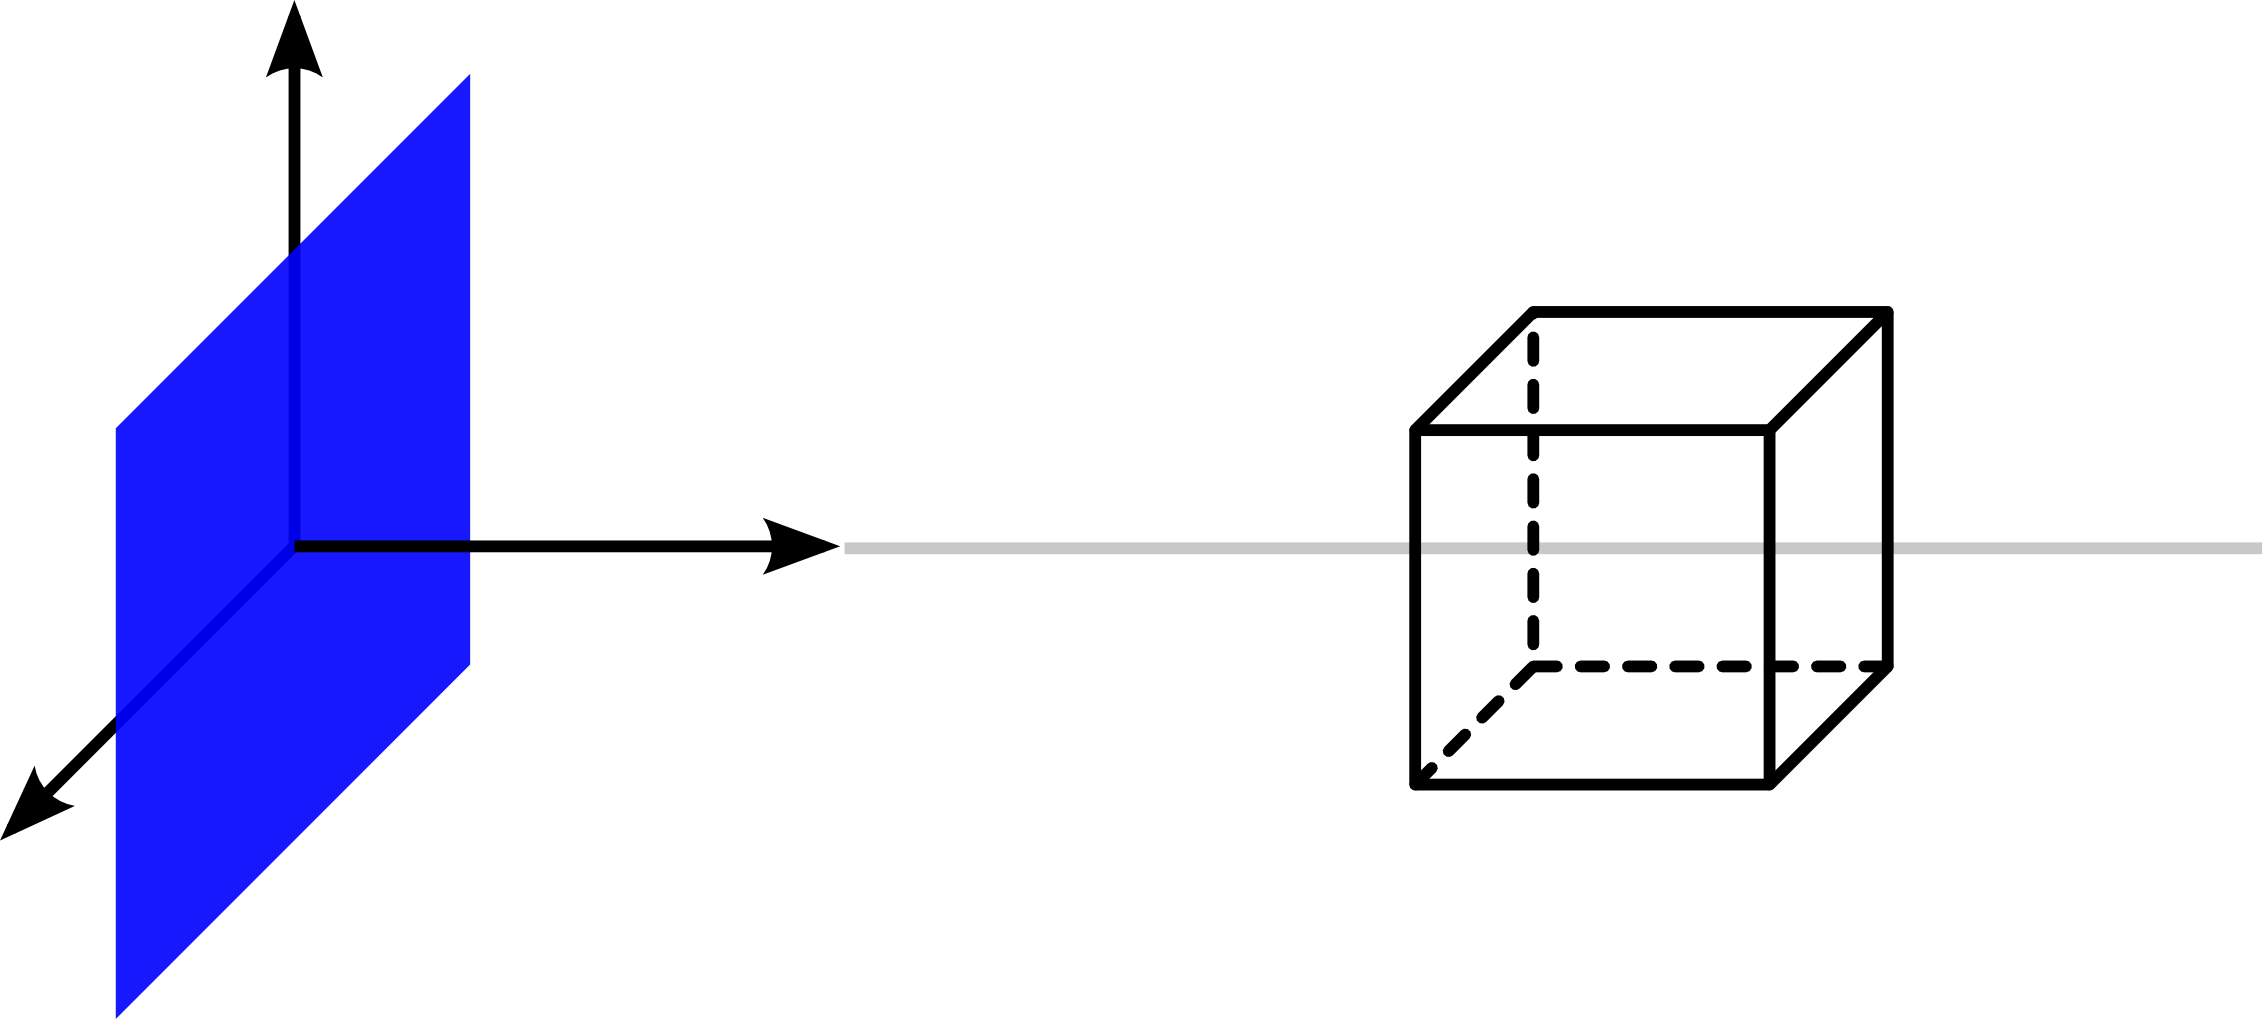
\includegraphics[width=70mm]{mass_diffusion0.png}}
    \put(9, 12){$0$}
    \put(57, 18){\setlength{\fboxsep}{0.4mm}\colorbox{white}{\scriptsize $dy$}}
    \put(43.5, 19.5){\setlength{\fboxsep}{0.4mm}\colorbox{white}{\scriptsize $dz$}}
    \put(48, 7){\setlength{\fboxsep}{0.4mm}\colorbox{white}{\scriptsize $dx$}}
    \put(16, 21){\color{bleu}$n_{i,1}$}
    \put(26, 14){\colorbox{white}{$x$}}
    \put( 8.5, 33){$y$}
    \put( -2,  3.5){$z$}
    \put(43, 5){$x$}
    \put(54, 5){$x+dx$}
  \end{picture}
\end{center}

\onslide<4>   

\begin{center}
  \begin{picture}(75, 35)(-10, -5)
    \put(  0, 0){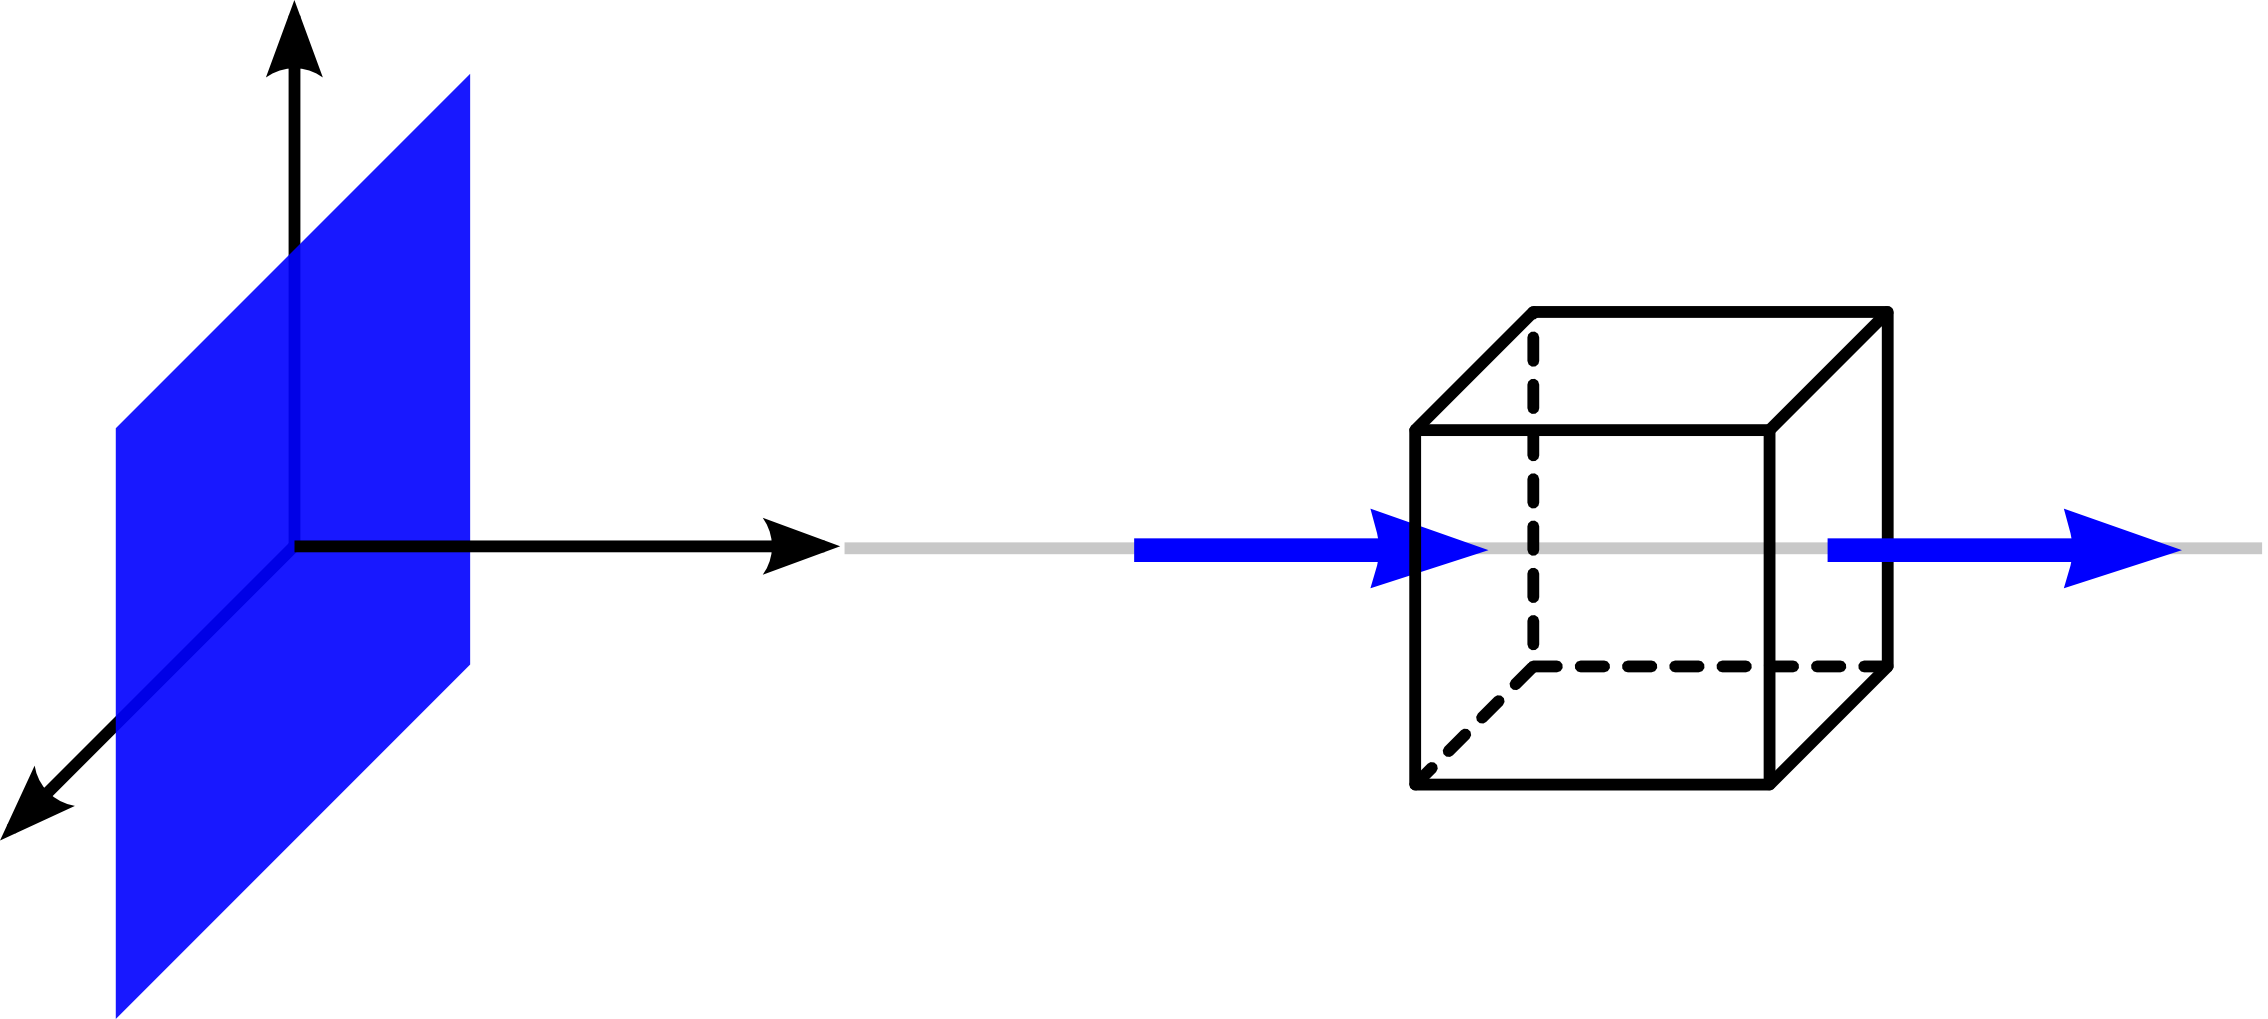
\includegraphics[width=70mm]{mass_diffusion1.png}}
    \put(9, 12){$0$}
    \put(57, 18){\setlength{\fboxsep}{0.4mm}\colorbox{white}{\scriptsize $dy$}}
    \put(43.5, 19.5){\setlength{\fboxsep}{0.4mm}\colorbox{white}{\scriptsize $dz$}}
    \put(48, 7){\setlength{\fboxsep}{0.4mm}\colorbox{white}{\scriptsize $dx$}}
    \put(16, 21){\color{bleu}$n_{i,1}$}
    \put(26, 14){\colorbox{white}{$x$}}
    \put( 8.5, 33){$y$}
    \put( -2,  3.5){$z$}
    \put(43, 5){$x$}
    \put(54, 5){$x+dx$}
    \put(30, 17){\color{bleu} flux $q_i(x, t)$}
    \put(61, 17){\color{bleu} flux $q_i(x+dx, t)$}
  \end{picture}
\end{center}

\end{overprint}

\vspace{-5mm}

\hspace{-5mm}
\begin{minipage}{110mm}
\begin{itemize}
\item[]<2->
variation de la quantité de particules $N_i(x, t)$  de l'espèce $i$ contenues dans le volume de contrôle élémentaire (fixe)
$dx\,dy\,dz$ avec $dx\rightarrow 0$ :
\item[]<2->
$= N_i(x, t+dt) - N_i(x, t) = \color{rouge} n_i(x, t+dt)dxdydz - n_i(x, t)dxdydz$
\item[\hspace{-10mm}]<2->
o\`u $n_i(x, t)$ : densité volumique (quantité de particules de l'espèce $i$ par unité de volume)
\item[]<3->
$=$ nb de particules qui sont entrées $-$ nb de particules qui sont sorties pendant $dt$ à travers $dydz$
\item[\hspace{-10mm}]<4->
$= \color{rouge} q_i(x, t) dydz \; dt - q_i(x+dx, t) dydz \, dt$
\item[]<4->
o\`u $q_i(x, t)$ : flux de l'espèce $i$ (nb de particules (ou de moles) de l'espèce $i$ qui traversent par unité de surface et par unité de temps)
\item[]<4->
\item[]<4->
\hfill \slshape \color{bleu} 
	NB : convention $q_i>0$ si flux vers les $x$ croissants, $q_i<0$ sinon.
\end{itemize}
\end{minipage}



\vspace{0.4mm}

\end{frame}

\begin{frame}{Diffusion de masse}
%--------------------------------------------------------------------------------------------------

\small

%\vspace{1mm}

\textbf{(a) Bilan de masse}

\begin{center}
  \begin{picture}(75, 32.2)(-10, -5)
    \put(  0, 0){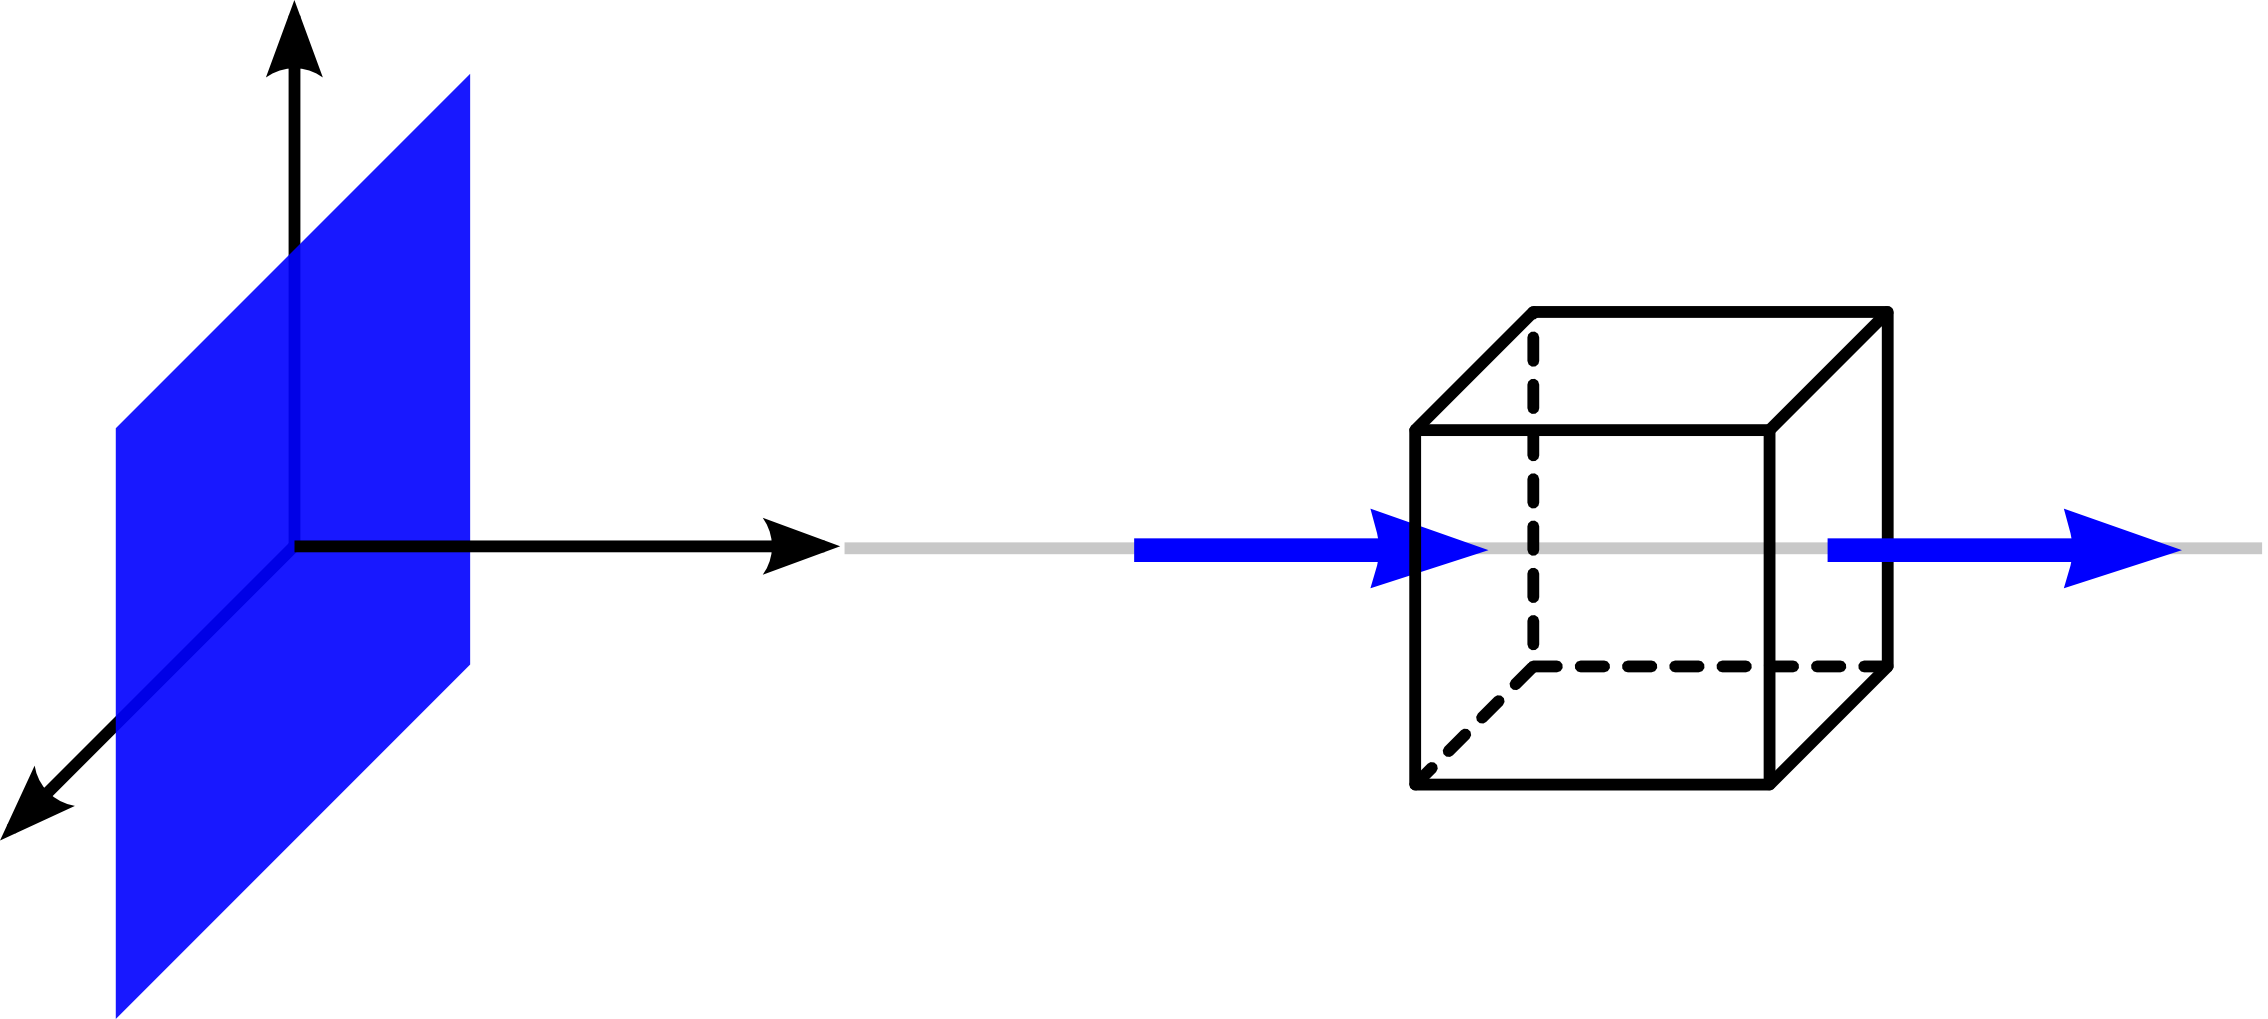
\includegraphics[width=70mm]{mass_diffusion1.png}}
    \put(9, 12){$0$}
    \put(57, 18){\setlength{\fboxsep}{0.4mm}\colorbox{white}{\scriptsize $dy$}}
    \put(43.5, 19.5){\setlength{\fboxsep}{0.4mm}\colorbox{white}{\scriptsize $dz$}}
    \put(48, 7){\setlength{\fboxsep}{0.4mm}\colorbox{white}{\scriptsize $dx$}}
    \put(16, 21){\color{bleu}$n_{i,1}$}
    \put(26, 14){\colorbox{white}{$x$}}
    \put( 8.5, 33){$y$}
    \put( -2,  3.5){$z$}
    \put(43, 5){$x$}
    \put(54, 5){$x+dx$}
    \put(30, 17){\color{bleu} flux $q_i(x, t)$}
    \put(61, 17){\color{bleu} flux $q_i(x+dx, t)$}
  \end{picture}
\end{center}

\vspace{-5mm}

En divisant par $dxdydz\,dt$ et en faisant tendre $dx$ et $dt$ vers 0 : \qquad
$
	\color{rouge} \dpdt{n_i} = - \dpdx{q_i}
$

\pause

\medskip

\textbf{(b) Loi de comportement} \medskip

Loi de Fick : le flux de matière est donné par \qquad
$
	\color{rouge}  q_i = -D \dpdx{n_i}
$

\begin{overprint}

\onslide<3>
o\`u $D$ : coefficient de diffusion massique ou moléculaire ou diffusivité (m$^2$/s).

\smallskip
Exemples : \smallskip


H$_2$O dans air : $D=2\; 10^{-6}$ m$^2$/s (gaz)

sucre dans eau : $D=5\; 10^{-10}$ m$^2$/s, ou sel dans eau : $D = 10^{-9}$ m$^2$/s (liquides)

carbone C dans Fe : $D = 10^{-12}$ m$^2$/s (solides)

\onslide<4>

\medskip

\textbf{(c) Equation de diffusion de la masse} \medskip

\onslide<5>

\medskip

\textbf{(c) Equation de diffusion de la masse} \medskip

\hspace{40mm} $\Rightarrow$ On en déduit : \qquad $\color{rouge}\dpdt{n_i} = D \ddpdx{n_i}$

\medskip

(= équation de diffusion instationnaire (1D), équation linéaire aux dérivées partielles)

\end{overprint}

\vspace{0mm}

\end{frame}
}

\comment{

%--------------------------------------------------------------------------------------------------
\subsubsection{Diffusion de quantité de mouvement}

\begin{frame}{Diffusion de quantité de mouvement}
%--------------------------------------------------------------------------------------------------

\small

\textbf{Objectif :} 

\medskip

dériver l'\textcolor{rouge}{équation d'évolution} associée à la mise en mouvement suivant $y$
d'un fluide visqueux initialement au repos.

\vspace{50mm}

\end{frame}




\begin{frame}{Diffusion de quantité de mouvement}
%--------------------------------------------------------------------------------------------------

\small

\textbf{(a) Bilan de quantité de mouvement}

\begin{center}
  \begin{picture}(75, 33)(-23, -5)
    \put(  0, 0){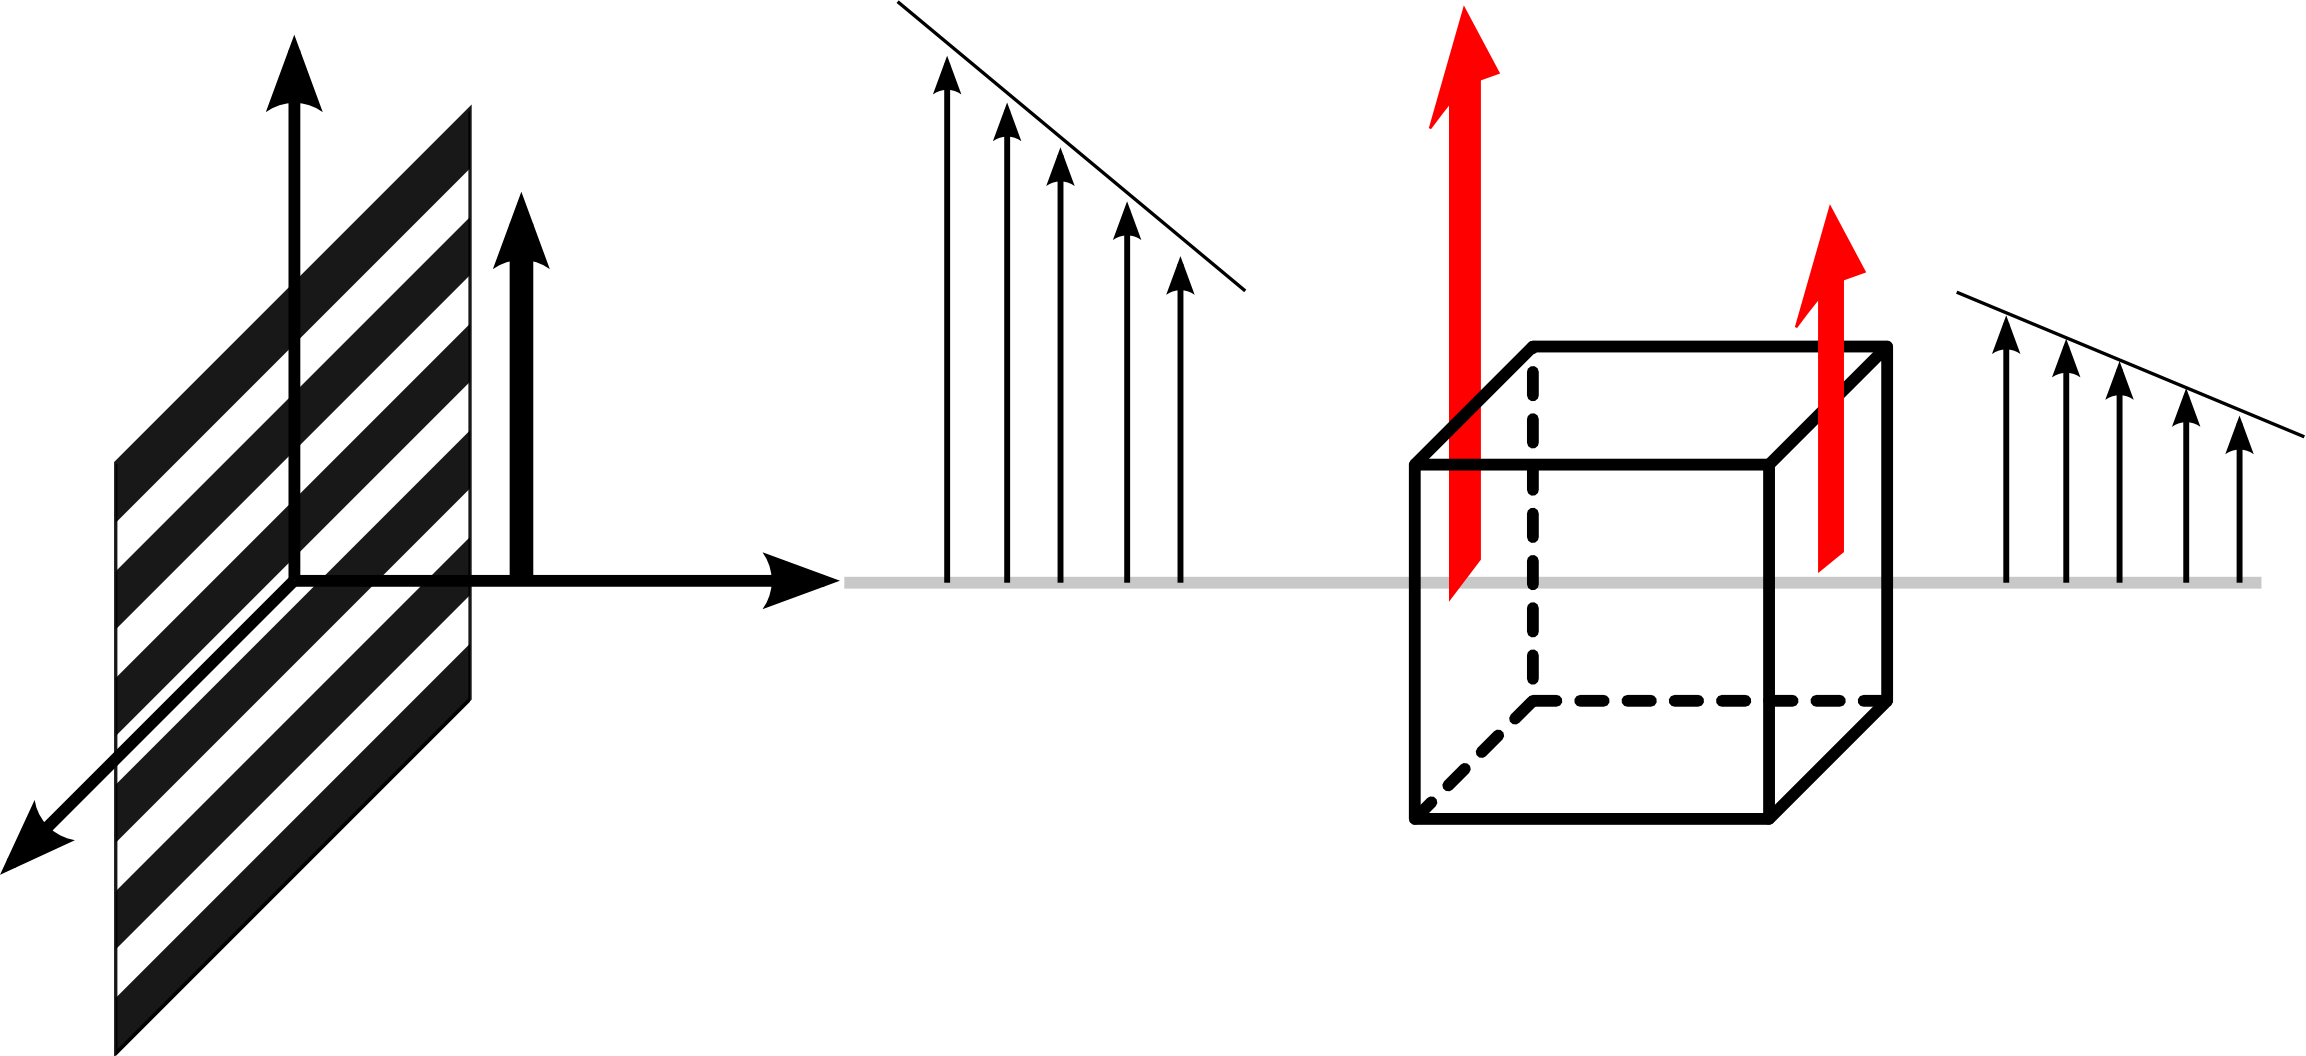
\includegraphics[width=70mm]{momentum_diffusion1.png}}
    \put(17, 22){$U_1$}
    \put(33, 29){\color{rouge}$\tau_{xy}(x, t)$}
    \put(50, 27){\color{rouge}$\tau_{xy}(x+dx, t)$}
    \put(25.5, 14){\setlength{\fboxsep}{0.4mm}\colorbox{white}{$x$}}
    \put( 8.5, 33){$y$}
    \put( -2,  3.5){$z$}
    \put(42, 5){$x$}
    \put(53, 5){$x+dx$}
  \end{picture}
\end{center}

\vspace{-5mm}

En divisant par $dxdydz\,dt$ et en faisant tendre $dx$ et $dt$ vers 0 : \qquad
$
	\color{rouge} \rho \dpdt{v} = \dpdx{\tau_{xy}}
$

\pause

\medskip

\textbf{(b) Loi de comportement} \medskip

Loi de Newton : la contrainte visqueuse est donnée par \qquad
$
	\color{rouge} \tau_{xy} = \mu \dpdx{v}
$

\begin{overprint}

\onslide<3>
o\`u $\mu$ : viscosité dynamique (Pa.s).

\smallskip
Exemples : H$_2$O : $\mu=10^{-3}$ Pa.s, \quad air (sec) : $\mu=18 \times 10^{-6}$ Pa.s

\onslide<4>

\medskip

\textbf{(c) Equation de diffusion de la quantité de mouvement} \medskip

\onslide<5>

\medskip

\textbf{(c) Equation de diffusion de la quantité de mouvement} \smallskip

\hspace{40mm} $\Rightarrow$ On en déduit : \qquad $\color{rouge} \dpdt{v} = \nu \ddpdx{v}$

\medskip

o\`u $\nu = \mu/\rho$ : coefficient de diffusion cinématique ou viscosité cinématique (m$^2$/s).

\smallskip
Exemples : H$_2$O : $\nu=10^{-6}$ m$^2$/s, \quad air (sec) : $\nu=15 \times 10^{-6}$ m$^2$/s

\end{overprint}

\vspace{1mm}

\end{frame}



%--------------------------------------------------------------------------------------------------
\subsubsection{Lois de comportement : justifications}

\begin{frame}{\insertsubsubsectionhead}



\pause

Loi de Fick :  \qquad $	\color{rouge}  q_i = -D \dpdx{n_i}$
\medskip

Loi de Newton : \qquad  $\color{rouge} \tau_{xy} = \mu \dpdx{v}$

\medskip

Loi de Fourier : \qquad $\color{rouge}	q = -\lambda \dpdx{T}$

\pause
\bigskip 

{\bf  Justifications :}
\medskip
\begin{itemize}[<+-| alert@+>]
\item Historiquement : lois établies de manière empirique

\item Pour les gaz : justification dans le cadre de la théorie cinétique 

\item[]
$$
D = \frac{ \bar{v} \ell}{3} ; \qquad 
\nu = \frac{ \bar{v} \ell}{3} ; \qquad 
\kappa = \frac{ \bar{v} \ell}{2}
$$
$\bar{v}$ = échelle de vitesse de l'agitation moléculaire ($\approx v_q$) ; $\ell$ libre parcours moyen.



\item Pour les liquides : pas de modèles simples.
\end{itemize}


\end{frame}

%--------------------------------------------------------------------------------------------------
\subsubsection{Longueur et temps caractéristiques de diffusion}

\begin{frame}{\insertsubsubsectionhead}
%--------------------------------------------------------------------------------------------------

\pause

\small

En désignant par $\phi(x, t)$ indifféremment les quantités $n_i(x, t)$, $u(y, t)$ ou $T(x, t)$,
\\
l'équation de transport par diffusion s'écrit

$$
\color{rouge} \dpdt{\phi} = d \, \ddpdx{\phi}
$$
\medskip
o\`u $d$ désigne la diffusivité de la quantité concernée ($d = D$, $\nu$ ou $\kappa$).

\medskip

\pause

L'\textbf{analyse dimensionnelle} de cette équation générique met en évidence 
une \textcolor{rouge}{échelle de longueur caractéristique} $\delta$ :

$$
	\frac{[\phi]}{t} \sim d \, \frac{[\phi]}{\delta^2}
$$

D'o\`u la loi de diffusion :
$$
	\color{vert} \delta(t) \sim \sqrt{d\, t}
$$

qui donne une bonne estimation de la longueur de pénétration observée dans les expériences.

\bigskip

\pause

En inversant cette relation, on montre que l'\textcolor{rouge}{échelle de temps caractéristique} 
de diffusion $\tau_d$ est donné par

$$
	\color{vert} \tau_d \sim L^2/d
$$

Ce temps caractéristique donne une estimation du temps nécessaire au processus de diffusion 
pour transporter la quantité concernée sur une distance $L$.

\end{frame}

%--------------------------------------------------------------------------------------------------
\begin{frame}{\insertsubsubsectionhead}
%--------------------------------------------------------------------------------------------------

\small

On remarquera que la diffusion est rapide aux temps courts, et plus lente aux temps longs :

\begin{center}
	\begin{picture}(70, 45)
		\put(10, 0){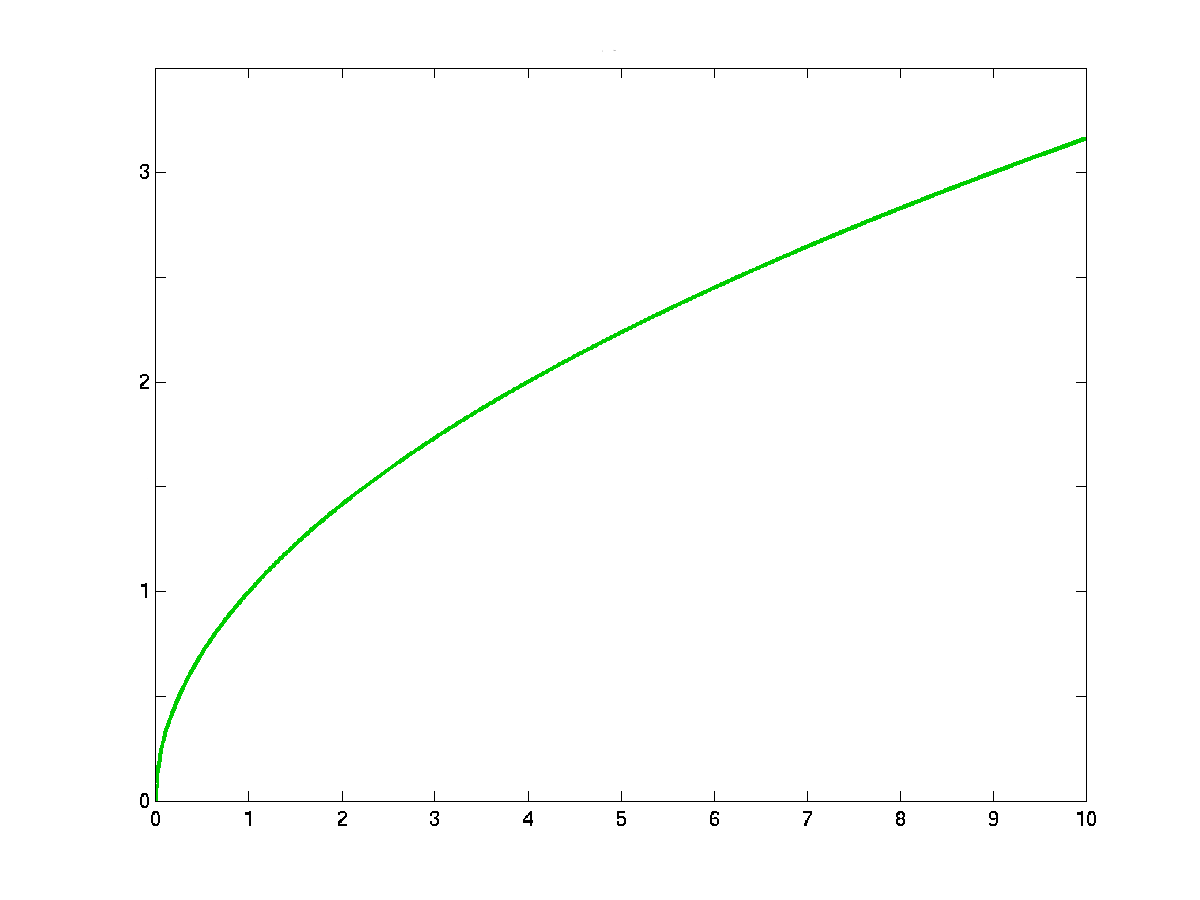
\includegraphics[width=60mm]{delta.png}}
		\put(10, 16){\vector(1, -1){8}}
		\put(-1, 18){cinétique rapide}
		\put(68, 28){\vector(-1, 1){8}}
		\put(66, 25){cinétique lente}
		\put(40, 0){$d\times t$}
		\put(0, 30){\large \color{vert}$\delta = \sqrt{d\, t}$}
	\end{picture}
\end{center}

\bigskip

\pause

\textcolor{rouge}{Application} : chauffage d'une cabine spatiale ($\kappa = 10^{-5}$ m$^2$/s)

\medskip

\qquad
$\rightarrow$ 
$\delta(\mbox{1 s.}) = 0.3$ cm, $\delta(\mbox{1 min.}) = 2.4$ cm, $\delta(\mbox{1 h.}) = 19$ cm, $\delta(\mbox{24 h.}) = 93$ cm


\vspace{0mm}

\end{frame}

%--------------------------------------------------------------------------------------------------
\subsubsection{Retour sur les expériences}

\begin{frame}{\insertsubsubsectionhead}
%--------------------------------------------------------------------------------------------------

\small

\textbf{Objectif :}

\medskip

Résoudre analytiquement l'équation de transport par diffusion

$$
\dpdt{\phi} = d \, \ddpdx{\phi}
$$

\medskip
pour les trois cas observés précédemment (masse, quantité de mouvement, énergie interne).

\bigskip

(cf. \textcolor{vert}{premier problème de Stokes} dans le cas de la quantité de mouvement)

\bigskip

\hfill \textcolor{rouge}{[$\longrightarrow$ exercice complémentaire]}

\vspace{35mm}

\end{frame}


%\end{document}

%==================================================================================================
\subsection{Transport par advection}
%==================================================================================================

%--------------------------------------------------------------------------------------------------
\begin{frame}{Notion d'advection et temps caractéristique}
%--------------------------------------------------------------------------------------------------

\small

La masse d'une espèce $i$, la quantité de mouvement d'un fluide ou son énergie interne peuvent être
simplement transportées par \textcolor{rouge}{déplacement de la matière à l'échelle macroscopique}, comme dans le cas
d'un fluide en écoulement par exemple, qui peut transporter de l'énergie interne (chaleur) en déplaçant 
du fluide chaud d'un point à un autre.

\bigskip
\pause

Si $U$ désigne la vitesse caractéristique de l'écoulement, on peut estimer l'ordre de grandeur du
temps nécessaire pour transporter par advection à vitesse $U$ une certaine quantité sur une distance donnée $L$ : 
\[
\color{vert}
	\tau_a = \frac{L}{U}
\]
$\tau_a$ représente le \textcolor{rouge}{temps caractéristique du processus d'advection}.

\bigskip
\pause

Inversement, pendant un temps donné $t$, le transport par advection permet de déplacer une quantité physique
sur une distance $$ \color{vert}\delta_a = U\, t$$

\vspace{20mm}

\end{frame}

%==================================================================================================
\subsection{Comparaison advection/diffusion}
%==================================================================================================

%--------------------------------------------------------------------------------------------------
\subsubsection{Efficacité relative}

\begin{frame}{\insertsubsubsectionhead}
%--------------------------------------------------------------------------------------------------

\small

Compétition entre diffusion et advection pour le transport d'une quantité sur une distance $L$ :

%\begin{minipage}
%	\begin{center}
		\setlength{\unitlength}{0.7mm}
		\begin{picture}(90, 65)
			\put(0, 0){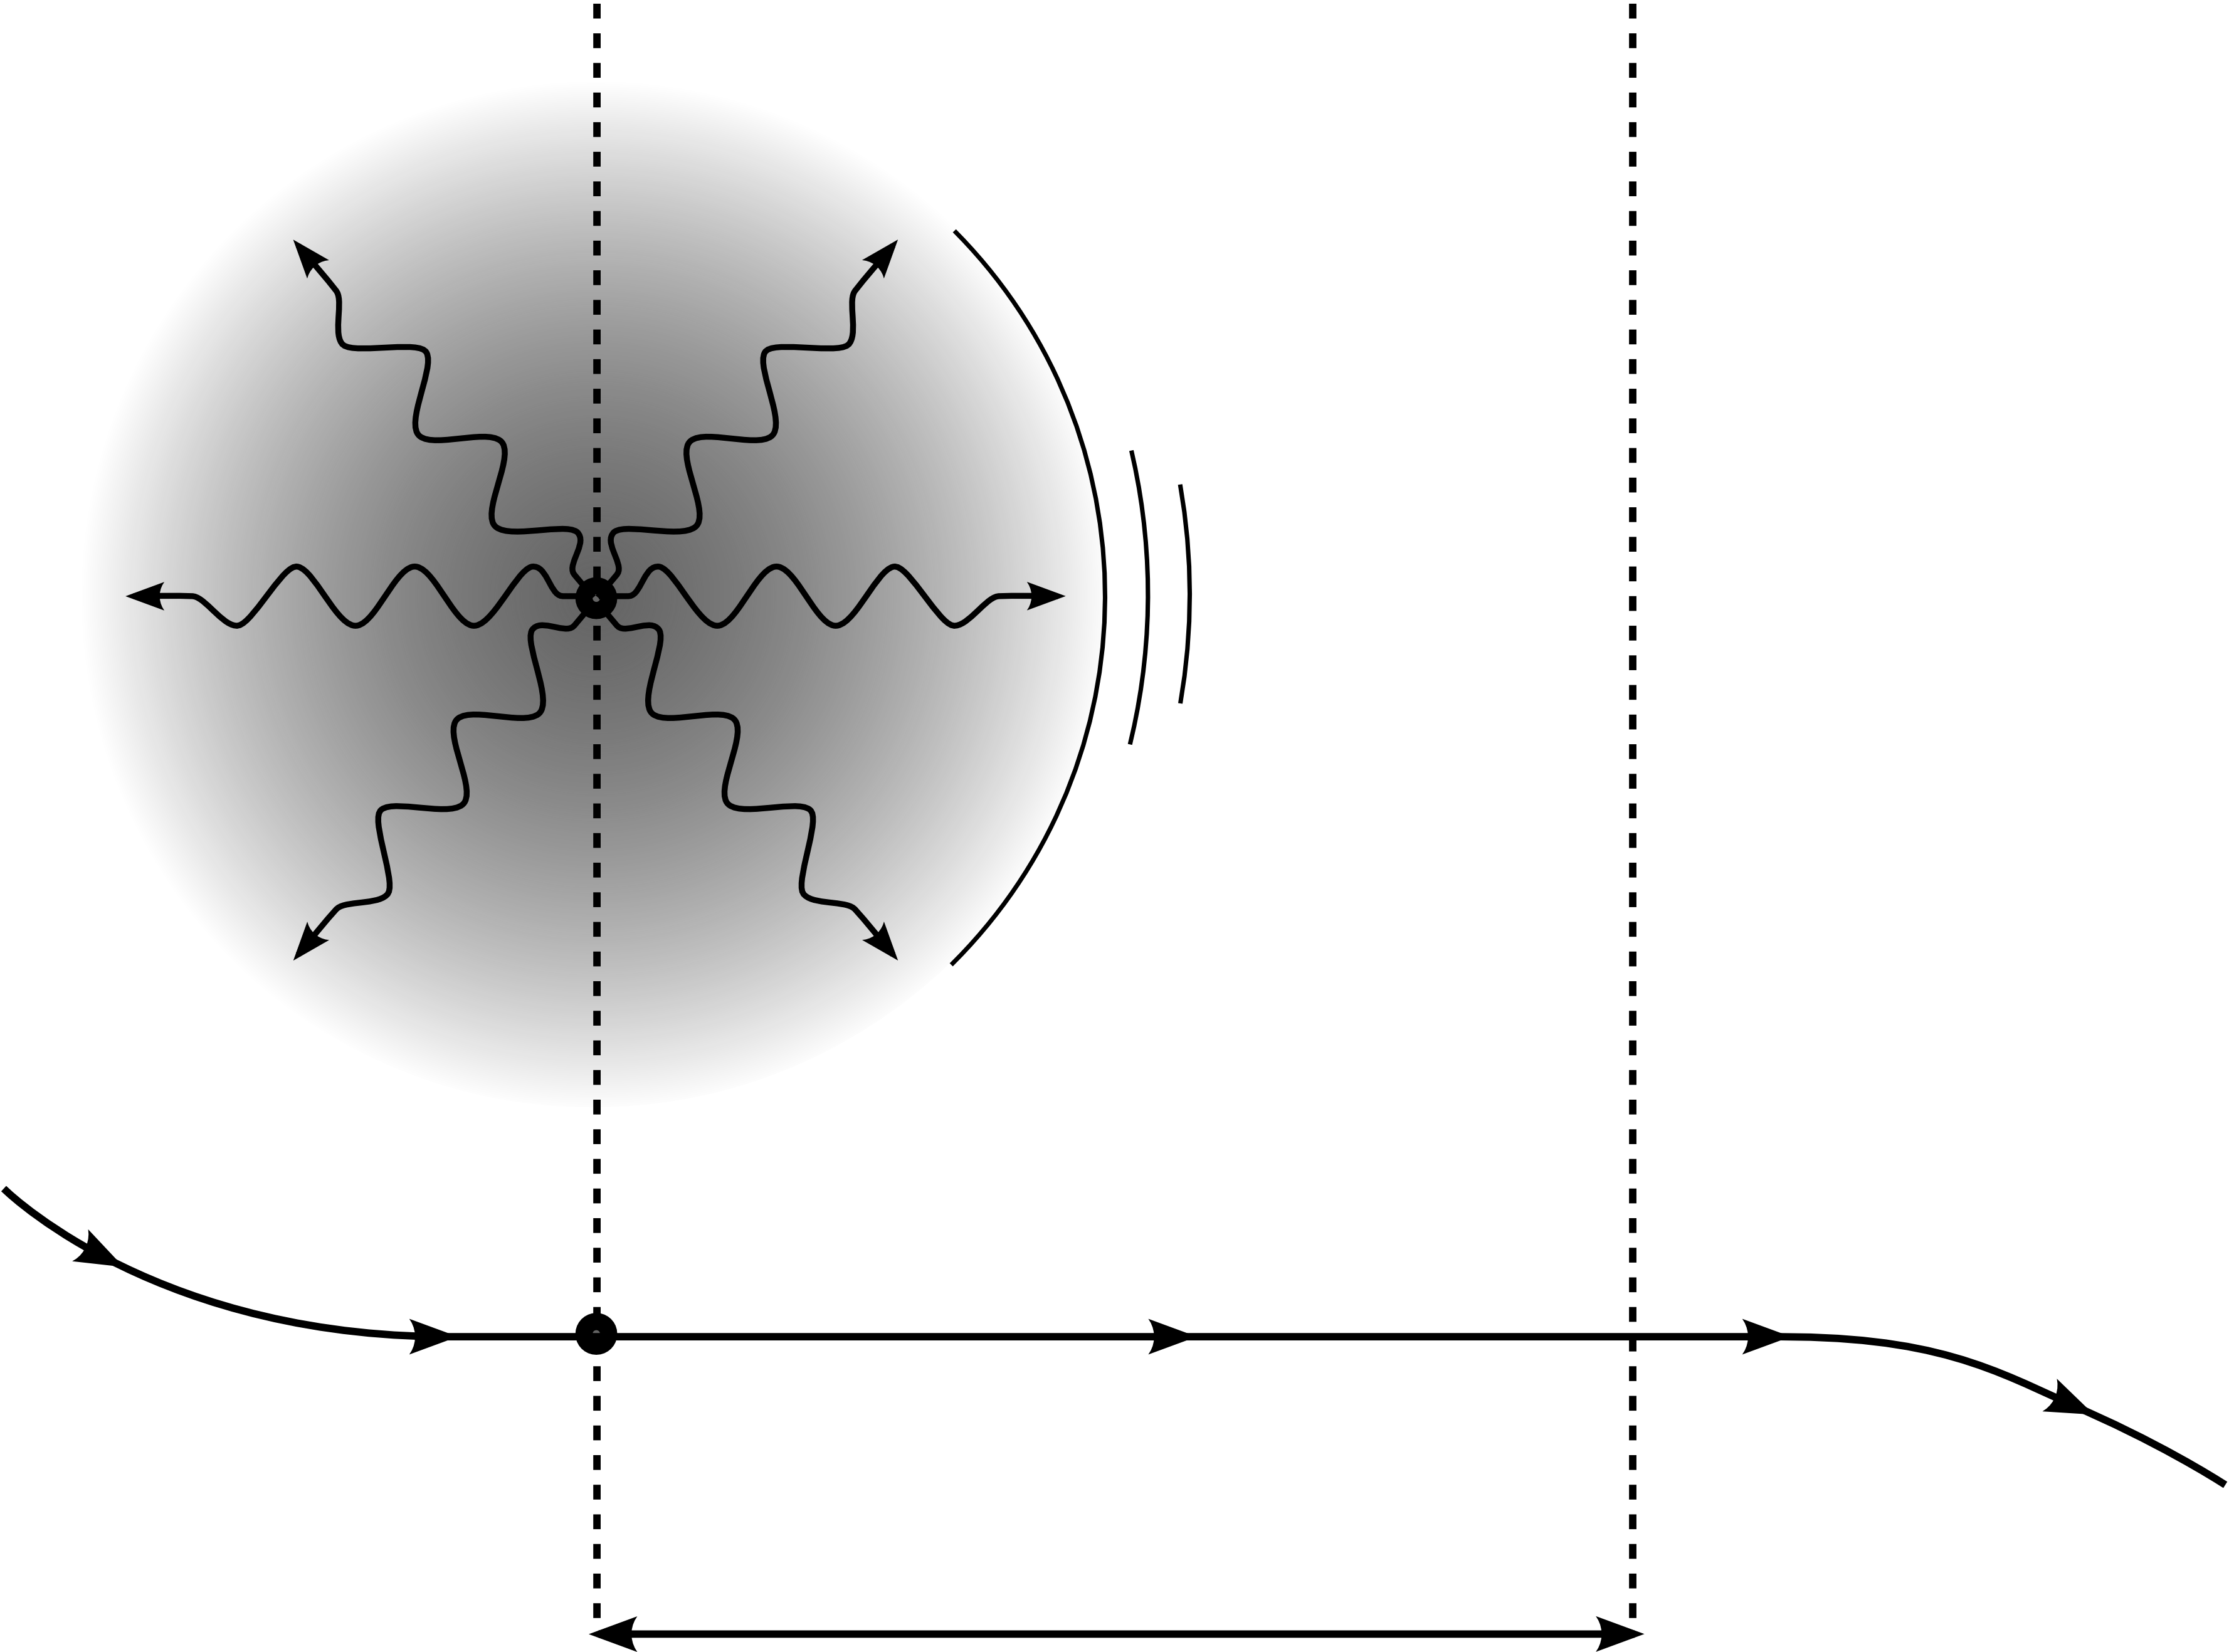
\includegraphics[width=63mm]{diffusion_advection.png}}	
			\put(46, 32){\footnotesize diffusion}
			\put(43, 28){\footnotesize(coefficient $d$)}
			\put(68, 32){\footnotesize temps \color{rouge} $\tau_d = L^2/d$}
			\put(28, 15){\footnotesize advection} 
			\put(28, 9){\footnotesize(vitesse $U$)}
			\put(68, 15){\footnotesize temps \color{vert} $\tau_a = L/U$}
			\put(43, 0){\footnotesize \colorbox{white}{$L$}}
		\end{picture}
		\qquad
		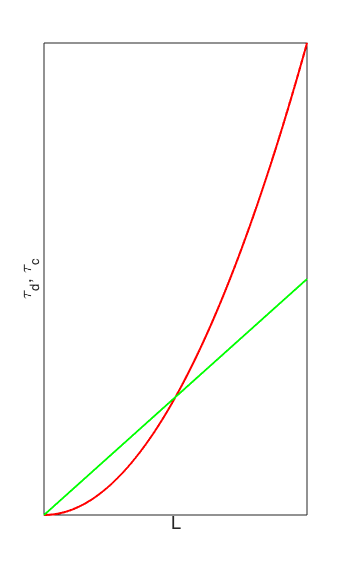
\includegraphics[width=30mm]{taudtaucL.png}
%	\end{center}
%\end{minipage}
	
	\medskip
	
	D'o\`u le rapport d'efficacité relative $ R = \dfrac{\tau_d}{\tau_a} = \dfrac{L^2/d}{L/U} = \dfrac{UL}{d}$ :
	  
	  
\medskip
	\qquad \color{rouge} Si $\tau_d \ll \tau_a \; \Leftrightarrow \; R \ll 1$ : 
	la diffusion est la plus efficace, l'advection est négligeable

\smallskip
	\qquad \color{vert} Si $\tau_d \gg \tau_a \; \Leftrightarrow \; R \gg 1$ : 
	l'advection est la plus efficace, la diffusion est négligeable

\end{frame}

%--------------------------------------------------------------------------------------------------
\subsubsection{Transport de masse}

\begin{frame}{\insertsubsubsectionhead}
%--------------------------------------------------------------------------------------------------

\small

Diffusion de masse : $d=D$ diffusivité moléculaire

\[
	\frac{\tau_d}{\tau_a} = \frac{L^2/D}{L/U} = \frac{UL}{D}
\]

\medskip

Ce rapport définit un paramètre sans dimension, le \textbf{nombre de Peclet} massique 
$$\color{vert}Pe_m = \frac{UL}{D}$$

\smallskip

Si $Pe_m\gg1$, alors $\tau_a\ll\tau_d$, et l'advection
est un mode de transport plus rapide, donc plus efficace, que la diffusion.
On peut alors négliger les phénomènes de diffusion massique dans la modélisation de ce type de configuration.

\smallskip

Si au contraire $Pe_m\ll1$, alors $\tau_a\gg\tau_d$ et c'est donc la diffusion qui est le mode de transport
dominant du problème étudié : on peut dans ce cas négliger l'advection.

\smallskip

En dehors de ces deux cas limites, les deux modes de transport doivent être pris en compte.

\vspace{22mm}

\end{frame}

%--------------------------------------------------------------------------------------------------
\subsubsection{Transport de quantité de mouvement}

\begin{frame}{\insertsubsubsectionhead}
%--------------------------------------------------------------------------------------------------

\small

Diffusion de quantité de mouvement : $d=\nu$ viscosité cinématique

\[
	\frac{\tau_d}{\tau_a} = \frac{L^2/\nu}{L/U} = \frac{UL}{\nu} 
\]

\medskip

Ce rapport définit un paramètre sans dimension, le \textbf{nombre de Reynolds}
\[
\color{vert}
	Re = \frac{UL}{\nu} = \rho \frac{UL}{\mu}
\]
o\`u $\mu = \rho \,\nu$ désigne la viscosité dynamique. 

\medskip

Le nombre de Reynolds est un paramètre fondamental en mécanique des fluides. 

\smallskip

Si \textcolor{rouge}{$Re\gg1$}, alors $\tau_a\ll\tau_d$, et l'advection
est un mode de transport plus rapide, donc plus efficace, que la diffusion.
On peut alors négliger les phénomènes de diffusion visqueuse dans la modélisation.
Ces écoulements dominés par le transport par advection, que l'on peut relier à l'inertie du fluide, 
sont appelés \textcolor{rouge}{écoulements inertiels}.

\smallskip

Si au contraire \textcolor{rouge}{$Re\ll1$}, 
alors $\tau_a\gg\tau_d$ et c'est donc la diffusion (\textit{i.e.} les frottements visqueux)
qui est le mode de transport dominant du problème étudié : on peut dans ce cas négliger l'advection
et on parle alors d'\textcolor{rouge}{écoulements visqueux}.

\vspace{15mm}

\end{frame}

%--------------------------------------------------------------------------------------------------
\subsubsection{Transport de chaleur}

\begin{frame}{\insertsubsubsectionhead}
%--------------------------------------------------------------------------------------------------

\small

Diffusion d'énergie interne (conduction thermique) : $d=\kappa$ diffusivité thermique

\[
	\frac{\tau_d}{\tau_a} = \frac{L^2/\kappa}{L/U} = \frac{UL}{\kappa} 
\]


\medskip

Ce rapport définit un paramètre sans dimension, le \textbf{nombre de Peclet} thermique 
$$\color{vert} Pe = \frac{UL}{\kappa}$$

\smallskip
Si \textcolor{rouge}{$Pe\gg1$}, alors $\tau_a\ll\tau_d$, et la convection
est un mode de transport plus rapide, donc plus efficace, que la conduction.
On peut alors négliger les phénomènes de conduction thermique dans la modélisation de ce type de configuration.
On parle alors de régime \textcolor{rouge}{convectif}.

\smallskip
Si au contraire \textcolor{rouge}{$Pe \ll1$}, alors $\tau_a\gg\tau_d$ et c'est donc la conduction qui est le mode de transport
dominant du problème étudié : on peut dans ce cas négliger l'advection (\textit{i.e.} la convection).
On parle alors de régime \textcolor{rouge}{conductif}.

\bigskip

\textbf{Remarque :} on peut aussi écrire
\[
	Pe = \frac{UL}{\kappa} = \frac{\nu}{\kappa} \; \frac{UL}{\nu} = Pr \; Re
\]
$Pr = \nu/\kappa$, rapport entre viscosité cinématique et diffusivité thermique, est le \textbf{nombre de Prandtl}.

\vspace{0mm}

\end{frame}

}

\comment{

%--------------------------------------------------------------------------------------------------
\begin{frame}{Diffusion de quantité de mouvement}
%--------------------------------------------------------------------------------------------------

\small

\textbf{(a) Bilan de quantité de mouvement}

\begin{overprint}

\onslide<1-2>   

\begin{center}
  \begin{picture}(75, 35)(-23, -5)
    \put(  0, 0){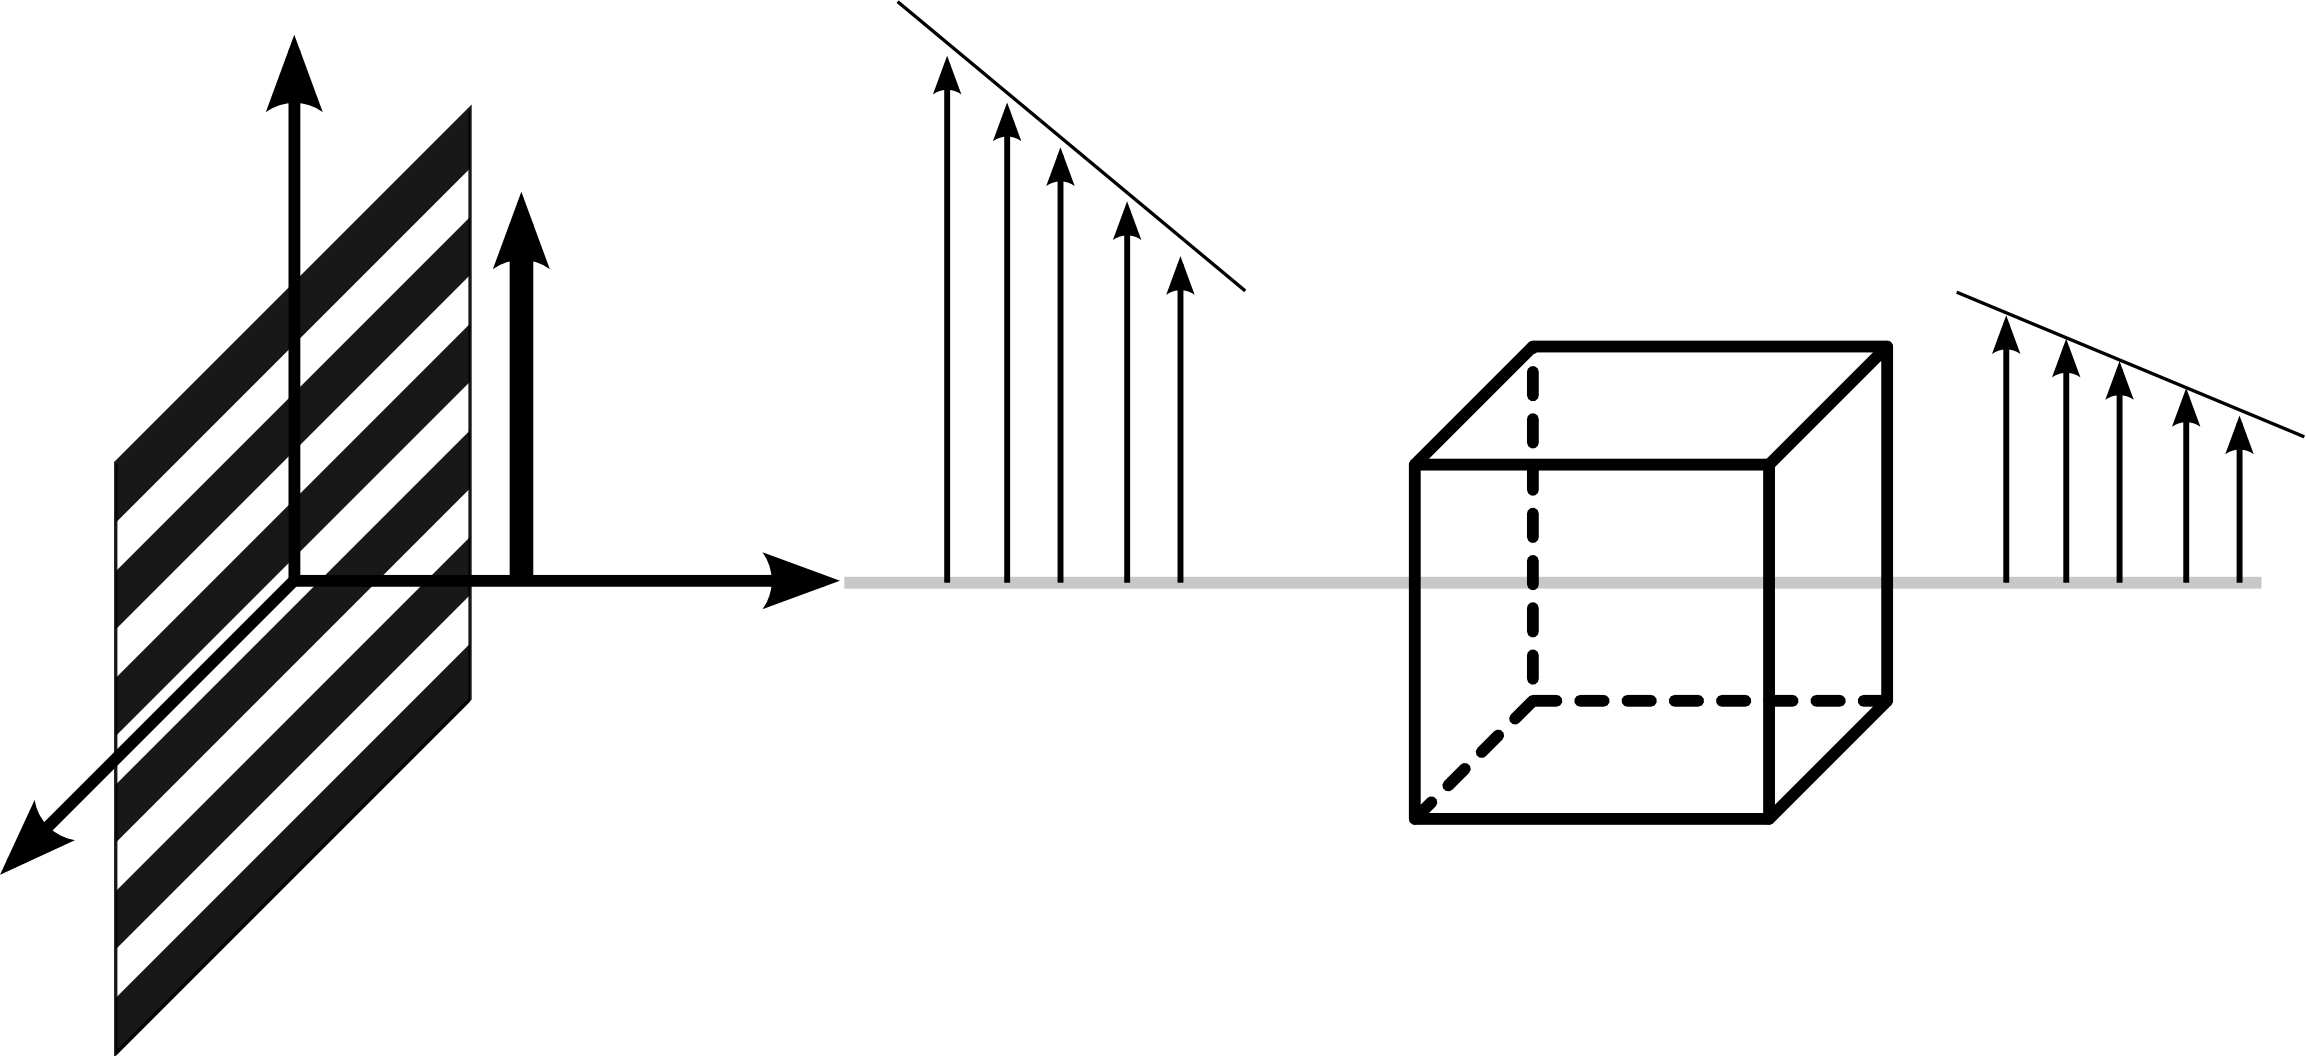
\includegraphics[width=70mm]{momentum_diffusion0.png}}
    \put(17, 22){$U_1$}
    \put(33, 29){$u(y, t)$}
    \put(56, 18){\setlength{\fboxsep}{0.4mm}\colorbox{white}{\scriptsize $dy$}}
    \put(43, 19.5){\setlength{\fboxsep}{0.4mm}\colorbox{white}{\scriptsize $dz$}}
    \put(48, 7){\setlength{\fboxsep}{0.4mm}\colorbox{white}{\scriptsize $dx$}}
    \put(25.5, 14){\setlength{\fboxsep}{0.4mm}\colorbox{white}{$x$}}
    \put( 8.5, 33){$y$}
    \put( -2,  3.5){$z$}
    \put(42, 5){$x$}
    \put(53, 5){$x+dx$}
  \end{picture}
\end{center}

\onslide<3>   

\begin{center}
  \begin{picture}(75, 35)(-23, -5)
    \put(  0, 0){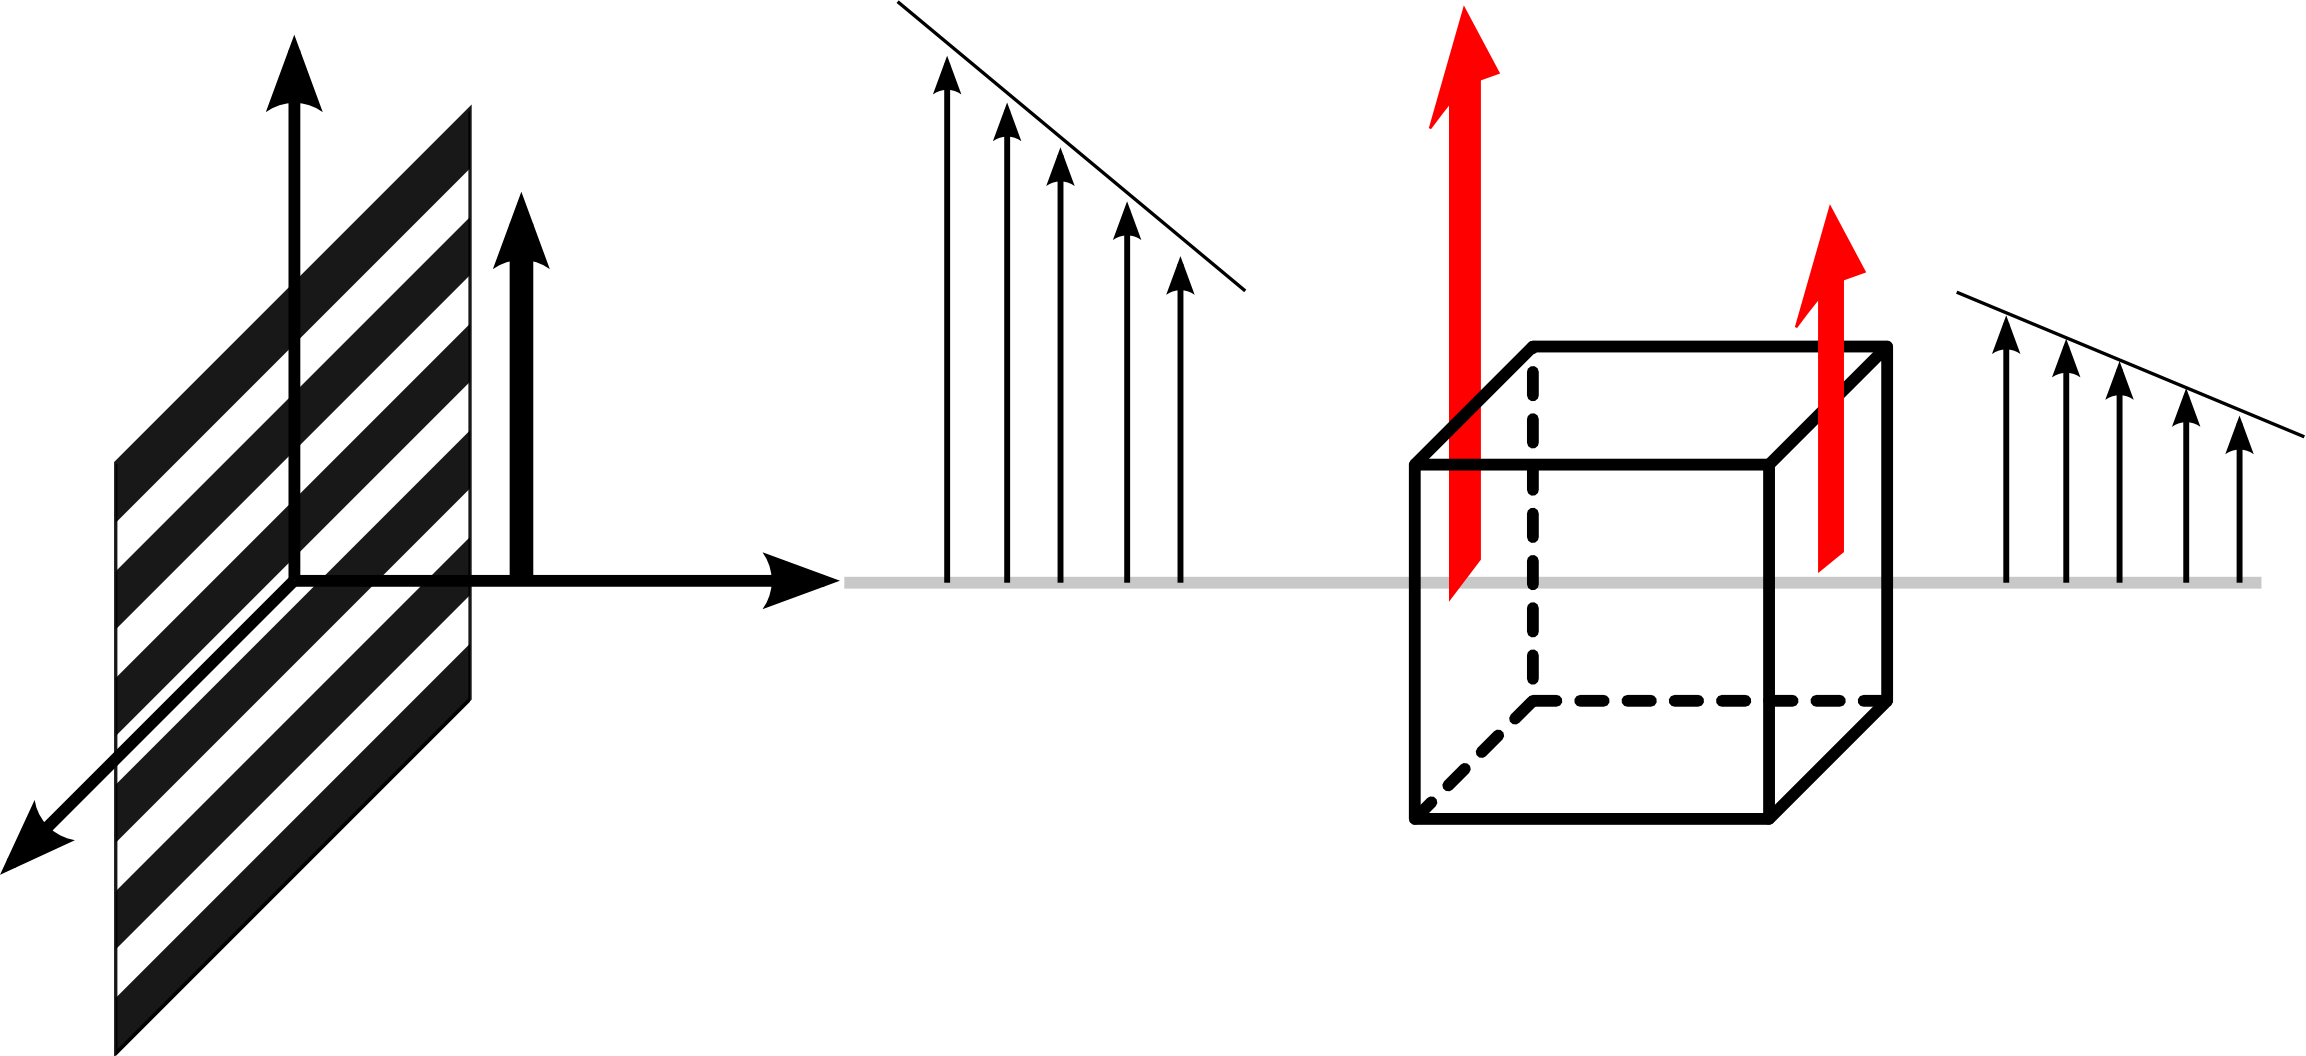
\includegraphics[width=70mm]{momentum_diffusion1.png}}
    \put(17, 22){$U_1$}
    \put(33, 29){\color{rouge}$\tau_{xy}(x, t)$}
    \put(50, 27){\color{rouge}$\tau_{xy}(x+dx, t)$}
    \put(25.5, 14){\setlength{\fboxsep}{0.4mm}\colorbox{white}{$x$}}
    \put( 8.5, 33){$y$}
    \put( -2,  3.5){$z$}
    \put(42, 5){$x$}
    \put(53, 5){$x+dx$}
  \end{picture}
\end{center}

\end{overprint}

\vspace{-1mm}

\begin{itemize}
\item[]<2->
Principe fondamental de la dynamique (PFD) dans la direction $y$ pour le fluide contenu dans le volume de contrôle élémentaire
$dx\,dy\,dz$ avec $dx\rightarrow 0$ :
\item[]<2->
$$\color{rouge} \rho \, dxdydz \, \dpdt{v}(x, t)= F_y(x, t) + F_y(x+dx, t)$$
\item[]<2->
$F_y$ : force suivant $y$ exercée par l'extérieur à travers $dydz$ sur le fluide à l'intérieur du volume 
\item[]<3->
avec $\color{rouge} F_y(x, t) = -\tau_{xy}(x, t) \, dydz$ 
et $\color{rouge} F_y(x+dx, t) = +\tau_{xy}(x+dx, t) \, dydz$
\item[]<3->
o\`u (cf. MMC) $\tau_{xy}(x, t)$ : contrainte suivant $y$ exercée sur la facette de normale $\myvec{e}_x$
\item[]<3->
\item[]<3->
\hfill \color{rouge}
\slshape NB : par convention la force est exercée par le milieu pointé par la normale
\end{itemize}

\vspace{4mm}

\end{frame}
}
\comment{
%--------------------------------------------------------------------------------------------------
\subsubsection{Modes de transport}

\begin{frame}{\insertsubsubsectionhead}
%--------------------------------------------------------------------------------------------------

\small

\textbf{Transporter comment ? } \medskip

Les trois \textcolor{rouge}{modes de transport} communément rencontrés sont :

\pause

\smallskip

\begin{itemize}[<+-| alert@+>]
\item
	la \textcolor{vert}{diffusion}, \textit{i.e.} le transport dû à l'agitation atomique 
	ou moléculaire à l'échelle microscopique.
\item[]
	Exemples : diffusion d'une goutte de lait dans du café au repos (masse); \\
	conduction thermique à travers la paroi de la tasse de café (énergie interne) ; \\
	ralentissement des mouvements du café dans la tasse après agitation avec une cuillère \\
	(diffusion visqueuse de la quantité de mouvement).
\item
	l'\textcolor{vert}{advection}, \textit{i.e.} le transport par le déplacement de la matière 
	à l'échelle macroscopique (fluide en écoulement par ex.).
\item[]
	Exemples : dispersion d'un nuage de polluants par le vent (masse); \\
	convection thermique naturelle/forcée/mixte au-dessus de la tasse de café (énergie interne); \\
	poussée d'un moteur fusée par éjection de gaz à travers une tuyère (quantité de mouvement);
\item
	le \textcolor{vert}{rayonnement} ou transport par des ondes, 
	un mode de transport spécifique à l'énergie.
\item[]
	Exemples : coup de soleil, effet de serre, etc (rayonnement thermique, ondes 		électromagnétiques).
	\\
	Rayonnement acoustique d'une trompette ou d'une guitare
	\\
	Récupération de l'énergie de la houle
	
\end{itemize}

\bigskip

\pause

Remarque : le transport de l'énergie interne par diffusion (conduction thermique), par advection (convection thermique) et par rayonnement fait l'objet du cours de Transferts thermiques.

\vspace{0mm}

\end{frame}

%==================================================================================================
\subsection{Transport par diffusion}
%==================================================================================================

%--------------------------------------------------------------------------------------------------
\subsubsection{Phénoménologie}

\begin{frame}{\insertsubsubsectionhead}
%--------------------------------------------------------------------------------------------------

\large

Considérons trois expériences élémentaires...

\bigskip



(Illustrations dans le cas d'un gaz 2D avec le programme {\sl kinetics.m} ) 

\bigskip


\vspace{30mm}

\end{frame}

%--------------------------------------------------------------------------------------------------
\begin{frame}{Expérience 1/3 : Diffusion d'une espèce chimique (i) dans un gaz}

%plaque peinte (pas sèche\ldots) en contact avec un fluide
%--------------------------------------------------------------------------------------------------

\small

\begin{overprint}

  \onslide<1>   

  \begin{center}
    \begin{picture}(100, 50)
    \put( 0, 0){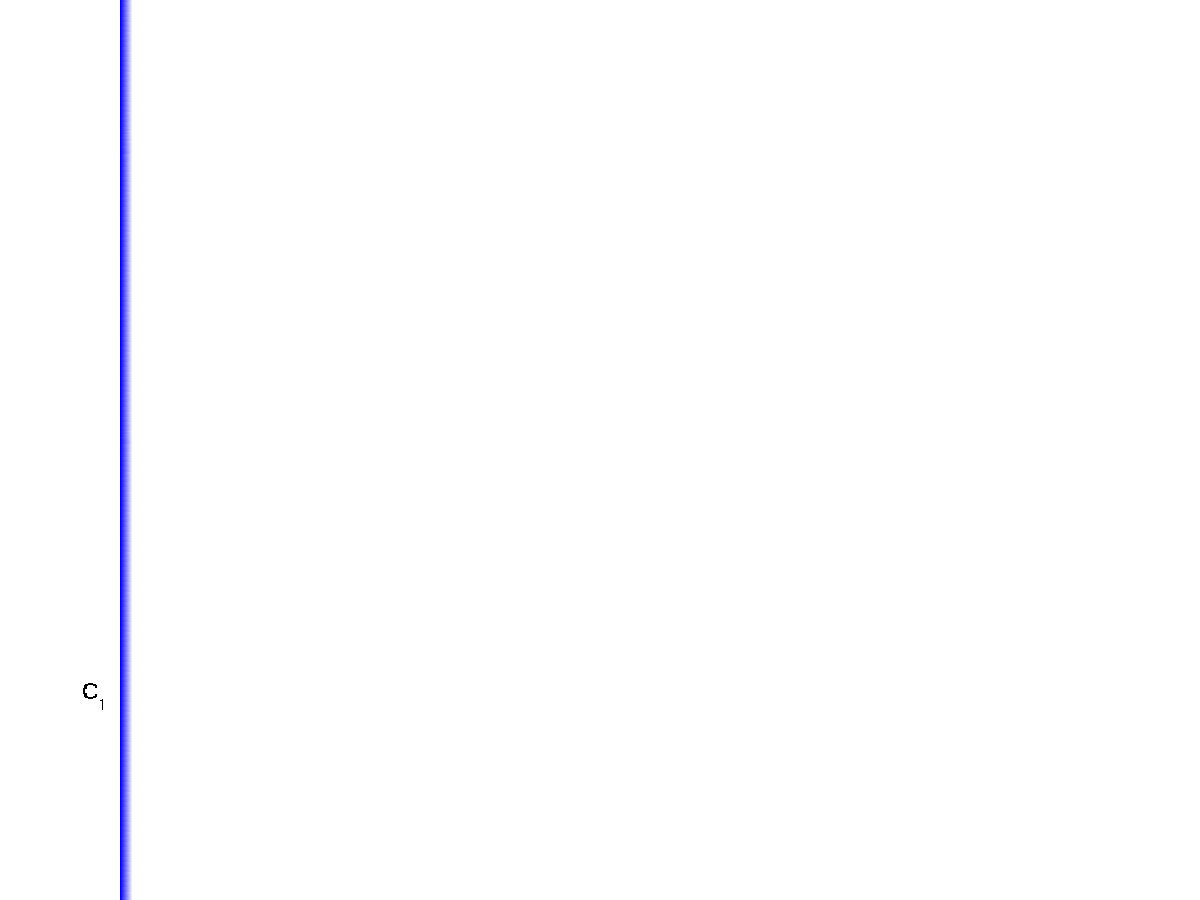
\includegraphics[width=50mm]{mass_diffusion_field0.png}}
    \put(40, 40){$t=0^-$}
    \put(-1, 22){$n_{i,1}$ }
    \put(10, 22){$n_i$ = 0}
    \put(2, 41){\color{rouge}membrane}
    \put(2, 39){\color{rouge}imperméable}
    \put(5.8, 0){\color{rouge}\line(0, 1){37.5}}
    \put(2.5, 8.5){\setlength{\fboxsep}{1mm}\colorbox{white}{}}
    \end{picture}
  \end{center}

  \onslide<2>   
  \begin{center}
    \begin{picture}(100, 50)
    \put( 0, 0){\movie[width=50mm,poster,externalviewer,showcontrols=false]{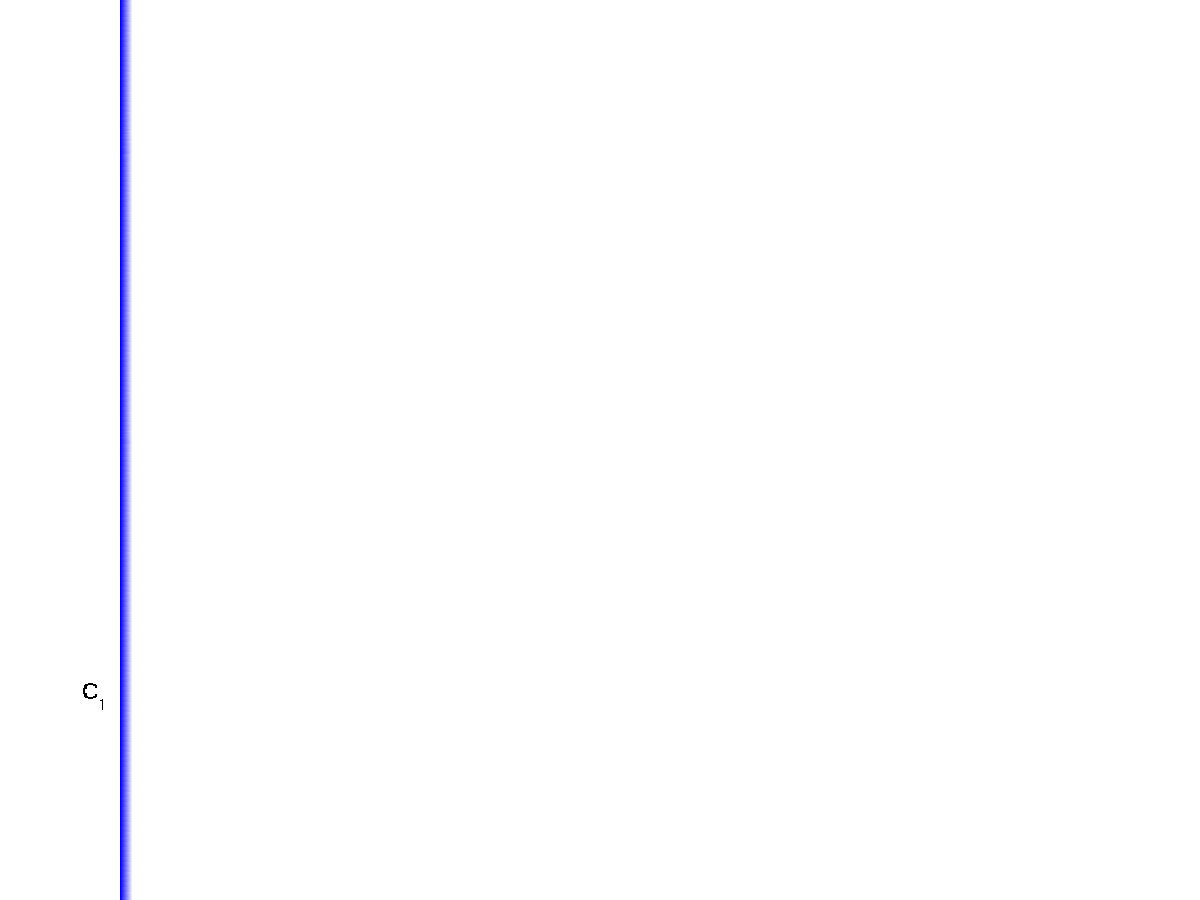
\includegraphics[width=50mm]{mass_diffusion_field0.png}}{./Figures/mass_diffusion.avi}}
    \put(40, 40){$t=0^+$}
    %\put(1,0){\vector(0, 1){20}}
    \put(-1, 22){$n_{i,1}$}
    \put(0, 19){\rotatebox{90}{$=$}}
    \put(-2, 16){$Cte$}
    \put(10, 22){$C_0=0$}
    \put(2.5, 8.5){\setlength{\fboxsep}{1mm}\colorbox{white}{}}
    \end{picture}
  \end{center}

  \onslide<3>   
  \begin{center}
    \begin{picture}(100, 50)
    \put( 0, 0){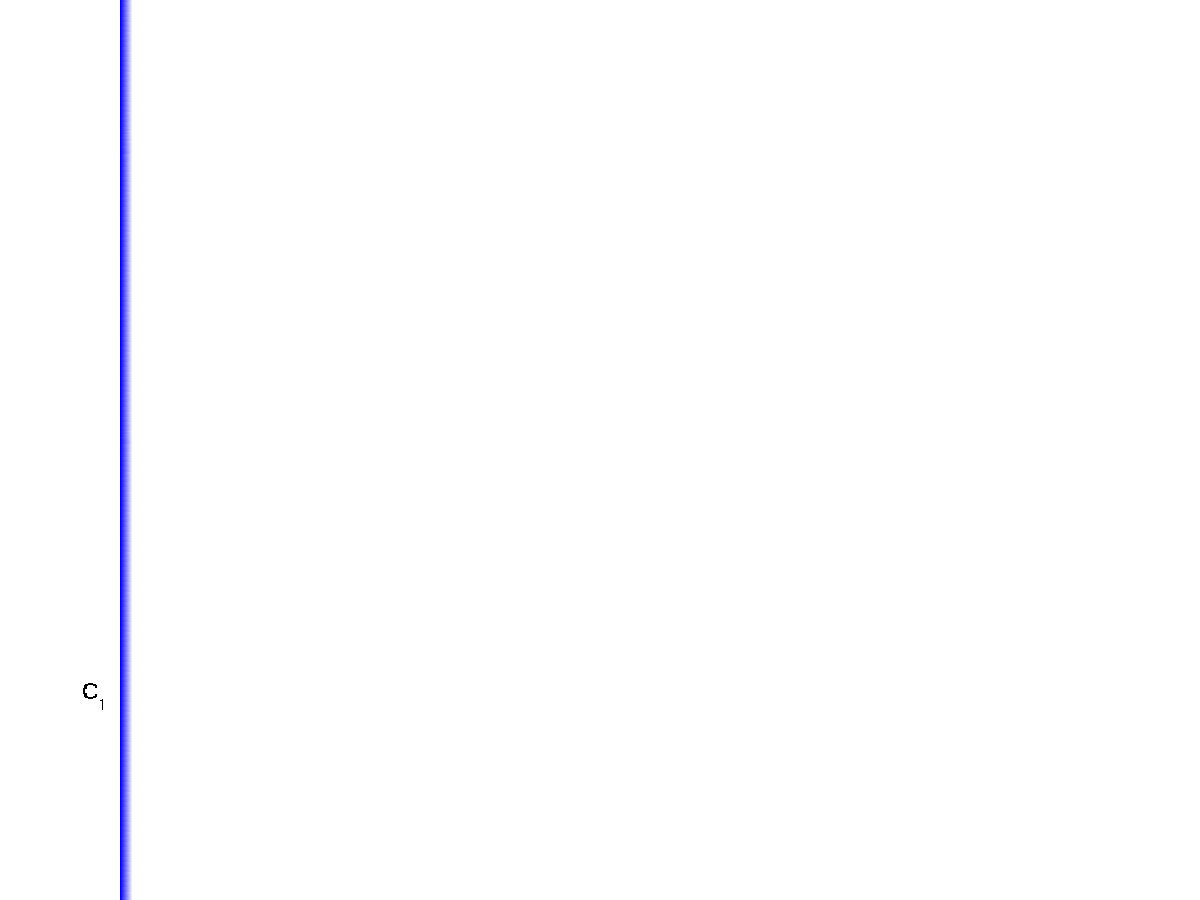
\includegraphics[width=50mm]{mass_diffusion_field0.png}}
    \put(55, 20){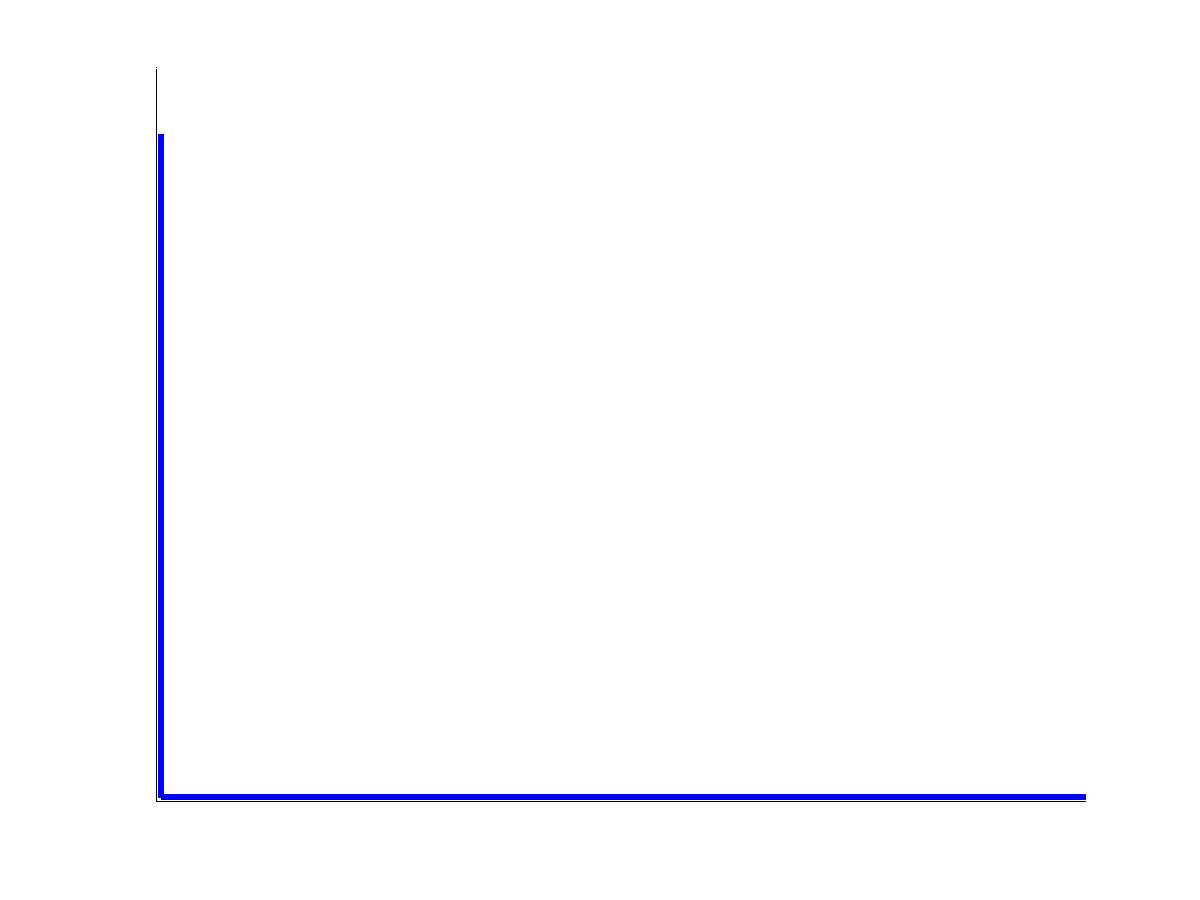
\includegraphics[width=45mm]{mass_diffusion_profile0.png}}
    \put(60.9, 51.2){\linethickness{0.01mm}\line(1, 0){34.75}}
    \put(95.75, 51.2){\linethickness{0.01mm}\line(0, -1){27.5}}
    \put(59, 23){$0$}
    \put(97, 23){$x$}
    \put(57, 48){$n_{i,1}$}
    \put(83, 46){$n_i(x,t)$}
    \put(40, 40){$t=0^+$}
    \put( 5, 10){\color{bleu} \line(1, 0){45}}
    \put(54, 10){\line(1, 0){10}}
    \put(64, 10){\vector(1, 1){10}}
    \put(73, 15){mesure du profil de}
    \put(72, 12){densité volumique $n_i(x,t)$}
    %\put(1,0){\vector(0, 1){20}}
    \put(-1, 22){$n_{i,1}$}
    \put(0, 19){\rotatebox{90}{$=$}}
    \put(-2, 16){$Cte$}
    \put(2.5, 8.5){\setlength{\fboxsep}{1mm}\colorbox{white}{}}
    \end{picture}
  \end{center}

  \onslide<4>   
  \begin{center}
    \begin{picture}(100, 50)
    \put( 0, 0){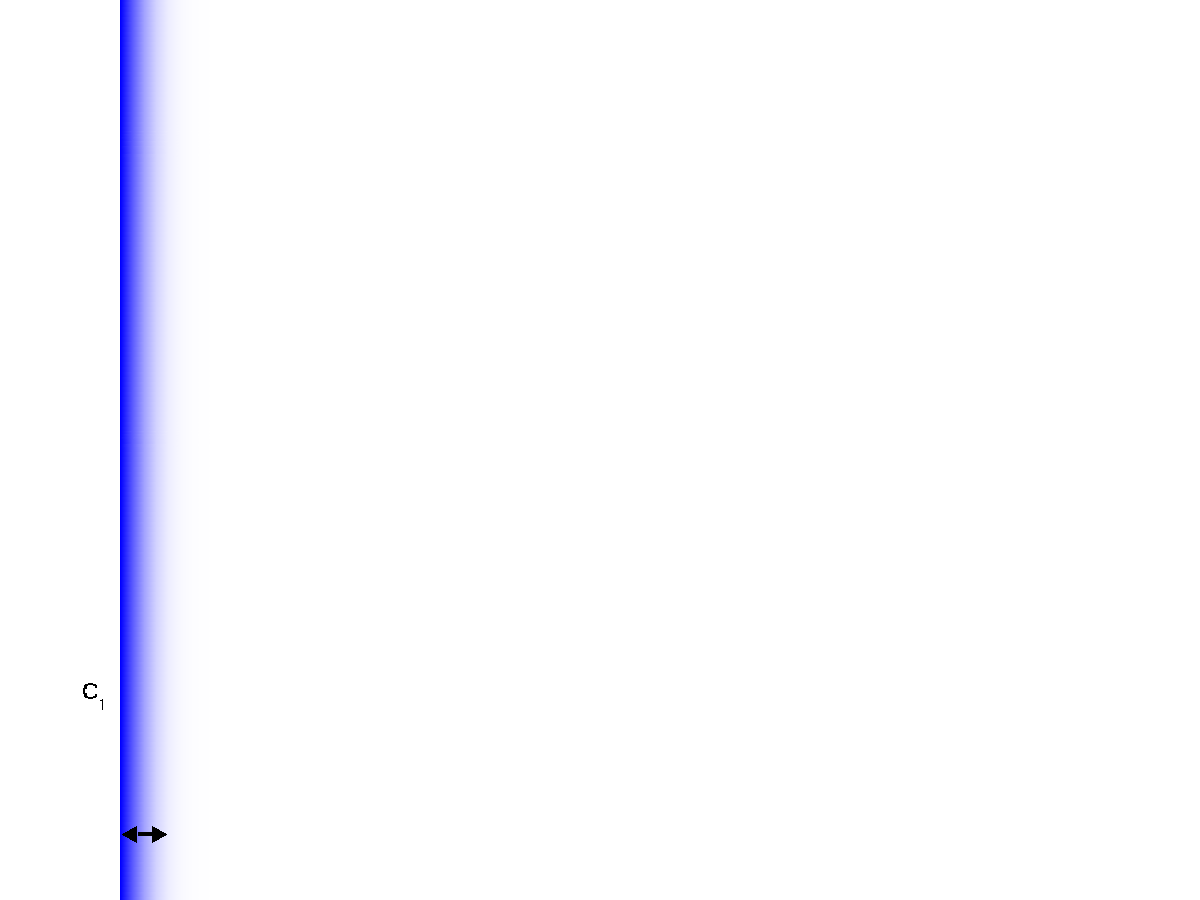
\includegraphics[width=50mm]{mass_diffusion_field1.png}}
    \put(55, 20){\includegraphics[width=45mm]{mass_diffusion_profile1.png}}
    \put(60.9, 51.2){\linethickness{0.01mm}\line(1, 0){34.75}}
    \put(95.75, 51.2){\linethickness{0.01mm}\line(0, -1){27}}
    \put(59, 23){$0$}
    \put(97, 23){$x$}
    \put(57, 48){$n_{i,1}$}
    \put(83, 46){$n_i(x,t)$}
    \put(40, 40){$t=t_1$}
    \put( 5, 10){\color{bleu} \line(1, 0){45}}
    \put(54, 10){\line(1, 0){10}}
    \put(64, 10){\vector(1, 1){10}}
    \put(73, 15){mesure du profil de}
    \put(72, 12){densité volumique $n_i(x,t)$}
    \put(62.3,25){\vector(1, 0){0} \scriptsize $\delta(t_1)$}
    \put(8,2.5){\scriptsize $\delta(t_1)$}
    \put(-1, 22){$n_{i,1}$}
    \put(0, 19){\rotatebox{90}{$=$}}
    \put(-2, 16){$Cte$}
    \put(2.5, 8.5){\setlength{\fboxsep}{1mm}\colorbox{white}{}}
    \end{picture}
  \end{center}

  \onslide<5>   
  \begin{center}
    \begin{picture}(100, 50)
    \put( 0, 0){\includegraphics[width=50mm]{mass_diffusion_field2.png}}
    \put(55, 20){\includegraphics[width=45mm]{mass_diffusion_profile2.png}}
    %\put(60.9, 51.2){\linethickness{0.01mm}\line(1, 0){34.75}}
    \put(59, 23){$0$}
    \put(97, 23){$x$}
    \put(57, 48){$n_{i,1}$}
    \put(83, 46){$n_i(x,t)$}
    \put(40, 40){$t=t_2$}
    \put( 5, 10){\color{bleu} \line(1, 0){45}}
    \put(54, 10){\line(1, 0){10}}
    \put(64, 10){\vector(1, 1){10}}
    \put(73, 15){mesure du profil de}
    \put(72, 12){densité volumique $n_i(x,t)$}
    \put(61,25){\vector(1, 0){2} \scriptsize $\delta(t_2)$}
    \put(9,2.5){\scriptsize $\delta(t_2)$}
    \put(-1, 22){$n_{i,1}$}
    \put(0, 19){\rotatebox{90}{$=$}}
    \put(-2, 16){$Cte$}
    \put(2.5, 8.5){\setlength{\fboxsep}{1mm}\colorbox{white}{}}
    \end{picture}
  \end{center}

  \onslide<6>   
  \begin{center}
    \begin{picture}(100, 50)
    \put( 0, 0){\includegraphics[width=50mm]{mass_diffusion_field3.png}}
    \put(55, 20){\includegraphics[width=45mm]{mass_diffusion_profile3.png}}
    %\put(60.9, 51.2){\linethickness{0.01mm}\line(1, 0){34.9}}
    \put(59, 23){$0$}
    \put(97, 23){$x$}
    \put(57, 48){$n_{i,1}$}
    \put(83, 46){$n_i(x,t)$}
    \put(40, 40){$t=t_3$}
    \put( 5, 10){\color{bleu} \line(1, 0){45}}
    \put(54, 10){\line(1, 0){10}}
    \put(64, 10){\vector(1, 1){10}}
    \put(73, 15){mesure du profil de}
    \put(72, 12){densité volumique $n_i(x,t)$}
    \put(61,25){\vector(1, 0){3} \scriptsize $\delta(t_3)$}
    \put(10,2.5){\scriptsize $\delta(t_3)$}
    \put(-1, 22){$n_{i,1}$}
    \put(0, 19){\rotatebox{90}{$=$}}
    \put(-2, 16){$Cte$}
    \put(2.5, 8.5){\setlength{\fboxsep}{1mm}\colorbox{white}{}}
    \end{picture}
  \end{center}

  \onslide<7>   
  \begin{center}
    \begin{picture}(100, 50)
    \put( 0, 0){\includegraphics[width=50mm]{mass_diffusion_field4.png}}
    \put(55, 20){\includegraphics[width=45mm]{mass_diffusion_profile4.png}}
    %\put(60.9, 51.2){\linethickness{0.01mm}\line(1, 0){34.9}}
    \put(59, 23){$0$}
    \put(97, 23){$x$}
    \put(57, 48){$n_{i,1}$}
    \put(83, 46){$n_i(x,t)$}
    \put(40, 40){$t=t_4$}
    \put( 5, 10){\color{bleu} \line(1, 0){45}}
    \put(54, 10){\line(1, 0){10}}
    \put(64, 10){\vector(1, 1){10}}
    \put(73, 15){mesure du profil de}
    \put(72, 12){densité volumique $n_i(x,t)$}
    \put(61,25){\vector(1, 0){4.5} \scriptsize $\delta(t_4)$}
    \put(11.5,2.5){\scriptsize $\delta(t_4)$}
    \put(-1, 22){$n_{i,1}$}
    \put(0, 19){\rotatebox{90}{$=$}}
    \put(-2, 16){$Cte$}
    \put(2.5, 8.5){\setlength{\fboxsep}{1mm}\colorbox{white}{}}
    \end{picture}
  \end{center}

  \onslide<8>   
  \begin{center}
    \begin{picture}(100, 50)
    \put( 0, 0){\includegraphics[width=50mm]{mass_diffusion_field5.png}}
    \put(55, 20){\includegraphics[width=45mm]{mass_diffusion_profile5.png}}
    %\put(60.9, 51.2){\linethickness{0.01mm}\line(1, 0){34.9}}
    \put(59, 23){$0$}
    \put(97, 23){$x$}
    \put(57, 48){$n_{i,1}$}
    \put(83, 46){$n_i(x,t)$}
    \put(40, 40){$t=t_5$}
    \put( 5, 10){\color{bleu} \line(1, 0){45}}
    \put(54, 10){\line(1, 0){10}}
    \put(64, 10){\vector(1, 1){10}}
    \put(73, 15){mesure du profil de}
    \put(72, 12){densité volumique $n_i(x,t)$}
    \put(61,25){\vector(1, 0){6.5} \scriptsize $\delta(t_5)$}
    \put(13.5,2.5){\scriptsize $\delta(t_5)$}
    \put(-1, 22){$n_{i,1}$}
    \put(0, 19){\rotatebox{90}{$=$}}
    \put(-2, 16){$Cte$}
    \put(2.5, 8.5){\setlength{\fboxsep}{1mm}\colorbox{white}{}}
    \end{picture}
  \end{center}

  \onslide<9>   
  \begin{center}
    \begin{picture}(100, 50)
    \put( 0, 0){\includegraphics[width=50mm]{mass_diffusion_field6.png}}
    \put(55, 20){\includegraphics[width=45mm]{mass_diffusion_profile6.png}}
    %\put(60.9, 51.2){\linethickness{0.01mm}\line(1, 0){34.9}}
    \put(59, 23){$0$}
    \put(97, 23){$x$}
    \put(57, 48){$n_{i,1}$}
    \put(83, 46){$n_i(x,t)$}
    \put(40, 40){$t=t_6$}
    \put( 5, 10){\color{bleu} \line(1, 0){45}}
    \put(54, 10){\line(1, 0){10}}
    \put(64, 10){\vector(1, 1){10}}
    \put(73, 15){mesure du profil de}
    \put(72, 12){densité volumique $n_i(x,t)$}
    \put(61,25){\vector(1, 0){10.5}}
    \put(72,25.5){\scriptsize $\delta(t_6)$}
    \put(17.5,2.5){\scriptsize $\delta(t_6)$}
    \put(-1, 22){$n_{i,1}$}
    \put(0, 19){\rotatebox{90}{$=$}}
    \put(-2, 16){$Cte$}
    \put(2.5, 8.5){\setlength{\fboxsep}{1mm}\colorbox{white}{}}
    \end{picture}
  \end{center}

  \onslide<10>   
  \begin{center}
    \begin{picture}(100, 50)
    \put( 0, 0){\includegraphics[width=50mm]{mass_diffusion_field7.png}}
    \put(55, 20){\includegraphics[width=45mm]{mass_diffusion_profile7.png}}
    %\put(60.9, 51.2){\linethickness{0.01mm}\line(1, 0){34.9}}
    \put(59, 23){$0$}
    \put(97, 23){$x$}
    \put(57, 48){$n_{i,1}$}
    \put(83, 46){$n_i(x,t)$}
    \put(40, 40){$t=t_7$}
    \put( 5, 10){\color{bleu} \line(1, 0){45}}
    \put(54, 10){\line(1, 0){10}}
    \put(64, 10){\vector(1, 1){10}}
    \put(73, 15){mesure du profil de}
    \put(72, 12){densité volumique $n_i(x,t)$}
    \put(61,25){\vector(1, 0){14.5}}
    \put(76,25.7){\scriptsize $\delta(t_7)$}
    \put(22,2.5){\scriptsize $\delta(t_7)$}
    \put(-1, 22){$n_{i,1}$}
    \put(0, 19){\rotatebox{90}{$=$}}
    \put(-2, 16){$Cte$}
    \put(2.5, 8.5){\setlength{\fboxsep}{1mm}\colorbox{white}{}}
    \end{picture}
  \end{center}

  \onslide<11>   
  \begin{center}
    \begin{picture}(100, 50)
    \put( 0, 0){\includegraphics[width=50mm]{mass_diffusion_field8.png}}
    \put(55, 20){\includegraphics[width=45mm]{mass_diffusion_profile8.png}}
    %\put(60.9, 51.2){\linethickness{0.01mm}\line(1, 0){34.9}}
    \put(59, 23){$0$}
    \put(97, 23){$x$}
    \put(57, 48){$n_{i,1}$}
    \put(83, 46){$n_i(x,t)$}
    \put(40, 40){$t=t_8$}
    \put( 5, 10){\color{bleu} \line(1, 0){45}}
    \put(54, 10){\line(1, 0){10}}
    \put(64, 10){\vector(1, 1){10}}
    \put(73, 15){mesure du profil de}
    \put(72, 12){densité volumique $n_i(x,t)$}
    \put(61,25){\vector(1, 0){20.5}}
    \put(81.5,25.8){\scriptsize $\delta(t_8)$}
    \put(28.5,2.5){\scriptsize $\delta(t_8)$}
    \put(-1, 22){$n_{i,1}$}
    \put(0, 19){\rotatebox{90}{$=$}}
    \put(-2, 16){$Cte$}
    \put(2.5, 8.5){\setlength{\fboxsep}{1mm}\colorbox{white}{}}
    \end{picture}
  \end{center}

  \onslide<12>   
  \begin{center}
    \begin{picture}(100, 50)
    \put( 0, 0){\includegraphics[width=50mm]{mass_diffusion_field9.png}}
    \put(55, 20){\includegraphics[width=45mm]{mass_diffusion_profile9.png}}
    %\put(60.9, 51.2){\linethickness{0.01mm}\line(1, 0){34.9}}
    \put(59, 23){$0$}
    \put(97, 23){$x$}
    \put(57, 48){$n_{i,1}$}
    \put(83, 46){$n_i(x,t)$}
    \put(40, 40){$t=t_9$}
    \put( 5, 10){\color{bleu} \line(1, 0){45}}
    \put(54, 10){\line(1, 0){10}}
    \put(64, 10){\vector(1, 1){10}}
    \put(73, 15){mesure du profil de}
    \put(72, 12){densité volumique $n_i(x,t)$}
    \put(61,25){\vector(1, 0){32.5}}
    \put(90,27){\scriptsize $\delta(t_9)$}
    \put(42,2.5){\scriptsize $\delta(t_9)$}
    \put(-1, 22){$n_{i,1}$}
    \put(0, 19){\rotatebox{90}{$=$}}
    \put(-2, 16){$Cte$}
    \put(2.5, 8.5){\setlength{\fboxsep}{1mm}\colorbox{white}{}}
    \end{picture}
  \end{center}

  \onslide<13>   
  \begin{center}
    \begin{picture}(100, 50)
    \put( 0, 0){\includegraphics[width=50mm]{mass_diffusion_field9.png}}
    \put(55, 20){\includegraphics[width=45mm]{mass_diffusion_profile9.png}}
    %\put(60.9, 51.2){\linethickness{0.01mm}\line(1, 0){34.9}}
    \put(59, 23){$0$}
    \put(97, 23){$x$}
    \put(57, 48){$n_{i,1}$}
    \put(83, 46){\color{rouge}$n_i(x,t)$}
%    \put(40, 40){$t=t_9$}
    \put( 5, 10){\color{bleu} \line(1, 0){45}}
    \put(54, 10){\line(1, 0){10}}
    \put(64, 10){\vector(1, 1){10}}
    \put(73, 15){mesure du profil de}
    \put(72, 12){densité volumique $n_i(x,t)$}
    \put(61,25){\color{rouge} \vector(1, 0){32.5}}
    \put(90,27){\color{rouge} $\delta(t)$}
    \put(42,2.5){\color{rouge} $\delta(t)$}
    \put(-1, 22){$n_{i,1}$}
    \put(0, 19){\rotatebox{90}{$=$}}
    \put(-2, 16){$Cte$}
%    \put(20, 5){\color{rouge}$\delta(t)$}
    \put(2.5, 8.5){\setlength{\fboxsep}{1mm}\colorbox{white}{}}
    \end{picture}
  \end{center}

\bigskip

  \hfill $\rightarrow$ Objectifs : déterminer l'évolution du profil de densité volumique 
  \textcolor{rouge}{$n_i(x,t)$} 
  et la loi de diffusion \textcolor{rouge}{$\delta(t)$}

\end{overprint}

\vspace{0mm}

\end{frame}


%%%%%%%%%%%%%%%%%%%%%%%%%%%%%%%%%%%%%%%%%%%%%%%%%%%%%%%%%%%%%%%%%%%%%%%%%%%%%%%%%%%%%%%%%%%%%%%%%%%
\section*{\bfseries Mécanismes de transport dans les fluides}
%%%%%%%%%%%%%%%%%%%%%%%%%%%%%%%%%%%%%%%%%%%%%%%%%%%%%%%%%%%%%%%%%%%%%%%%%%%%%%%%%%%%%%%%%%%%%%%%%%%

%==================================================================================================
\subsection{Phénomènes de transport}
%==================================================================================================

%--------------------------------------------------------------------------------------------------
\subsubsection{Notion de transport}

\begin{frame}{\insertsubsubsectionhead}
%--------------------------------------------------------------------------------------------------

\small

\textbf{Kézako ?} \medskip

En mécanique des fluides, et plus généralement en physique, chimie, biologie, ingénierie, etc.,
\\
on appelle \textcolor{rouge}{phénomène de transport} tout processus par lequel une quantité est déplacée d'un endroit à un autre.

\vspace{10mm}

\pause

\textbf{Transporter quoi ? } \medskip

Les \textcolor{rouge}{quantités} ou \textcolor{rouge}{grandeurs physiques} déplacées 
classiquement rencontrées en mécanique sont :

\pause

\smallskip

\begin{itemize}[<+-| alert@+>]
\item
	la \textcolor{vert}{masse} (d'une espèce $i$ dans un mélange)
\item
	la \textcolor{vert}{quantité de mouvement} (d'un fluide en écoulement)
\item
	l'\textcolor{vert}{énergie} 
	\begin{itemize}
	\item interne (la chaleur)
	\item mécanique 
	\end{itemize}
	
%\item
%	la \textcolor{vert}{charge électrique} (dans un plasma en MHD)
\item
  $[\ldots]$
\end{itemize}

%\pause

\vspace{15mm}

\end{frame}

\comment{
%--------------------------------------------------------------------------------------------------
\subsubsection{Diffusion d'énergie interne}


\begin{frame}{Diffusion d'énergie interne}
%--------------------------------------------------------------------------------------------------

\small

\textbf{Objectif :} 

\medskip

dériver l'\textcolor{rouge}{équation d'évolution} associée au réchauffement progressif d'un milieu
initialement à température uniforme.

\vspace{50mm}

\end{frame}

%--------------------------------------------------------------------------------------------------
\begin{frame}{Diffusion d'énergie interne}
%--------------------------------------------------------------------------------------------------

\small

\textbf{(a) Bilan d'énergie interne}

\begin{overprint}

\onslide<1-2>   

\begin{center}
  \begin{picture}(75, 35)(-10, -5)
    \put(  0, 0){\includegraphics[width=70mm]{heat_diffusion0.png}}
    \put(9, 12){$0$}
    \put(57, 18){\setlength{\fboxsep}{0.4mm}\colorbox{white}{\scriptsize $dy$}}
    \put(43.5, 19.5){\setlength{\fboxsep}{0.4mm}\colorbox{white}{\scriptsize $dz$}}
    \put(48, 7){\setlength{\fboxsep}{0.4mm}\colorbox{white}{\scriptsize $dx$}}
    \put(16, 21){\color{rouge}$T_1$}
    \put(26, 14){\colorbox{white}{$x$}}
    \put( 8.5, 33){$y$}
    \put( -2.5,  3.5){$z$}
    \put(43, 5){$x$}
    \put(54, 5){$x+dx$}
  \end{picture}
\end{center}

\onslide<3>   

\begin{center}
  \begin{picture}(75, 35)(-10, -5)
    \put(  0, 0){\includegraphics[width=70mm]{heat_diffusion1.png}}
    \put(9, 12){$0$}
    \put(57, 18){\setlength{\fboxsep}{0.4mm}\colorbox{white}{\scriptsize $dy$}}
    \put(43.5, 19.5){\setlength{\fboxsep}{0.4mm}\colorbox{white}{\scriptsize $dz$}}
    \put(48, 7){\setlength{\fboxsep}{0.4mm}\colorbox{white}{\scriptsize $dx$}}
    \put(16, 21){\color{rouge}$T_1$}
    \put(26, 14){\colorbox{white}{$x$}}
    \put( 8.5, 33){$y$}
    \put( -2.5,  3.5){$z$}
    \put(43, 5){$x$}
    \put(54, 5){$x+dx$}
    \put(31, 17){\color{rouge} flux $q(x, t)$}
    \put(61, 17){\color{rouge} flux $q(x+dx, t)$}
  \end{picture}
\end{center}

\end{overprint}

\vspace{-5mm}

\begin{itemize}
\item[]<2->
Premier principe de la thermodynamique pour le milieu contenu dans le volume de contrôle élémentaire
$dx\,dy\,dz$ (o\`u $E$ : énergie interne dans $dxdydz$, $E_k$ : énergie cinétique) :
$$ \color{rouge}
\ddt{}(E+E_k) = \mathcal{P}_{m, ext} + \mathcal{P}_{th} \qquad \mbox{cf. cours de Transferts thermiques}$$ 
\item[]<3->
Pour une tranche d'épaisseur $dx$ d'un milieu au repos ($E_k = 0$) et isovolume, 
$\mathcal{P}_{m, ext} = 0$ et l'équation pour l'énergie interne peut s'écrire :
$$
 \color{rouge} \rho C \dpdt{T} = -\dpdx{q}
$$ \\
o\`u $C$ désigne la capacité thermique et $q$ désigne le flux de chaleur 
(énergie interne qui passe par unité de surface et par unité de temps)
\item[]<3->
\item[]<3->
\hfill \color{rouge}
\slshape NB : convention $q>0$ si flux de chaleur vers les $x$ croissants, $q<0$ sinon.
\end{itemize}

\vspace{0mm}

\end{frame}

\begin{frame}{Diffusion d'énergie interne}
%--------------------------------------------------------------------------------------------------

\small

\textbf{(a) Bilan d'énergie interne}

\begin{center}
  \begin{picture}(75, 32)(-10, -5)
    \put(  0, 0){\includegraphics[width=70mm]{heat_diffusion1.png}}
    \put(9, 12){$0$}
    \put(57, 18){\setlength{\fboxsep}{0.4mm}\colorbox{white}{\scriptsize $dy$}}
    \put(43.5, 19.5){\setlength{\fboxsep}{0.4mm}\colorbox{white}{\scriptsize $dz$}}
    \put(48, 7){\setlength{\fboxsep}{0.4mm}\colorbox{white}{\scriptsize $dx$}}
    \put(16, 21){\color{rouge}$T_1$}
    \put(26, 14){\colorbox{white}{$x$}}
    \put( 8.5, 33){$y$}
    \put( -2.5,  3.5){$z$}
    \put(43, 5){$x$}
    \put(54, 5){$x+dx$}
    \put(31, 17){\color{rouge} flux $q(x, t)$}
    \put(61, 17){\color{rouge} flux $q(x+dx, t)$}
  \end{picture}
\end{center}

\vspace{-5mm}

Premier principe de la thermodynamique :
\qquad
$
\color{rouge} \rho C \dpdt{T} = -\dpdx{q}
$

\pause

\medskip

\textbf{(b) Loi de comportement} \medskip

Loi de Fourier : le flux de chaleur est donné par \qquad
$
\color{rouge}	q = -\lambda \dpdx{T}
$

o\`u $\lambda$ : conductivité thermique (W/m/K).

\pause

\medskip

\textbf{(c) Equation de diffusion de la chaleur} \medskip

\hspace{40mm} $\Rightarrow$ On en déduit : \qquad $\color{rouge}\dpdt{T} = \kappa \ddpdx{T}$

\medskip

o\`u $\kappa = \lambda/\rho C$ coefficient de diffusion thermique (ou diffusivité thermique, m$^2$/s).

\vspace{4mm}

\end{frame}
}



%--------------------------------------------------------------------------------------------------
\begin{frame}{Expérience 3/3 : plaque chauffée en contact avec un fluide ou un solide}
%--------------------------------------------------------------------------------------------------

\small

\begin{overprint}

  \onslide<1>   

  \begin{center}
    \begin{picture}(100, 50)
    \put( 0, 0){\includegraphics[width=50mm]{heat_diffusion_field0.png}}
    \put(40, 40){$t=0^-$}
    \put(-1, 22){$T_1$}
    \put(10, 22){\color{white}$T_0<T_1$}
    \put(2, 39){\color{vert}isolant}
    \put(5.8, 0){\color{vert}\line(0, 1){37.5}}
    \put(2.5, 8.5){\setlength{\fboxsep}{1mm}\colorbox{white}{}}
    \end{picture}
  \end{center}

  \onslide<2>   
  \begin{center}
    \begin{picture}(100, 50)
    \put( 0, 0){\movie[width=50mm,poster,externalviewer,showcontrols=false]{\includegraphics[width=50mm]{heat_diffusion_field0.png}}{./Figures/heat_diffusion.avi}}
    \put(40, 40){$t=0^+$}
    %\put(1,0){\vector(0, 1){20}}
    \put(-1, 22){$T_1$}
    \put(0, 19){\rotatebox{90}{$=$}}
    \put(-2, 16){$Cte$}
    \put(2.5, 8.5){\setlength{\fboxsep}{1mm}\colorbox{white}{}}
    \end{picture}
  \end{center}

  \onslide<3>   
  \begin{center}
    \begin{picture}(100, 50)
    \put( 0, 0){\includegraphics[width=50mm]{heat_diffusion_field0.png}}
    \put(55, 20){\includegraphics[width=45mm]{heat_diffusion_profile0.png}}
    \put(60.9, 51.2){\linethickness{0.01mm}\line(1, 0){34.75}}
    \put(95.75, 51.2){\linethickness{0.01mm}\line(0, -1){27.5}}
    \put(57, 23){$T_0$}
    \put(97, 23){$x$}
    \put(57, 48){$T_1$}
    \put(83, 46){$T(x, t)$}
    \put(40, 40){$t=0^+$}
    \put( 5, 10){\color{rouge} \line(1, 0){45}}
    \put(54, 10){\line(1, 0){10}}
    \put(64, 10){\vector(1, 1){10}}
    \put(73, 15){mesure du profil de}
    \put(72, 12){température $T(x, t)$}
    %\put(1,0){\vector(0, 1){20}}
    \put(-1, 22){$T_1$}
    \put(0, 19){\rotatebox{90}{$=$}}
    \put(-2, 16){$Cte$}
    \put(2.5, 8.5){\setlength{\fboxsep}{1mm}\colorbox{white}{}}
    \end{picture}
  \end{center}

  \onslide<4>   
  \begin{center}
    \begin{picture}(100, 50)
    \put( 0, 0){\includegraphics[width=50mm]{heat_diffusion_field1.png}}
    \put(55, 20){\includegraphics[width=45mm]{heat_diffusion_profile1.png}}
    \put(60.9, 51.2){\linethickness{0.01mm}\line(1, 0){34.75}}
    \put(95.75, 51.2){\linethickness{0.01mm}\line(0, -1){27}}
    \put(57, 23){$T_0$}
    \put(97, 23){$x$}
    \put(57, 48){$T_1$}
    \put(83, 46){$T(x, t)$}
    \put(40, 40){$t=t_1$}
    \put( 5, 10){\color{rouge} \line(1, 0){45}}
    \put(54, 10){\line(1, 0){10}}
    \put(64, 10){\vector(1, 1){10}}
    \put(73, 15){mesure du profil de}
    \put(72, 12){température $T(x, t)$}
    \put(62.3,25){\vector(1, 0){0} \scriptsize $\delta(t_1)$}
    \put(8,2.5){\scriptsize \color{yellow} $\delta(t_1)$}
    \put(-1, 22){$T_1$}
    \put(0, 19){\rotatebox{90}{$=$}}
    \put(-2, 16){$Cte$}
    \put(2.5, 8.5){\setlength{\fboxsep}{1mm}\colorbox{white}{}}
    \end{picture}
  \end{center}

  \onslide<5>   
  \begin{center}
    \begin{picture}(100, 50)
    \put( 0, 0){\includegraphics[width=50mm]{heat_diffusion_field2.png}}
    \put(55, 20){\includegraphics[width=45mm]{heat_diffusion_profile2.png}}
    %\put(60.9, 51.2){\linethickness{0.01mm}\line(1, 0){34.75}}
    \put(57, 23){$T_0$}
    \put(97, 23){$x$}
    \put(57, 48){$T_1$}
    \put(83, 46){$T(x, t)$}
    \put(40, 40){$t=t_2$}
    \put( 5, 10){\color{rouge} \line(1, 0){45}}
    \put(54, 10){\line(1, 0){10}}
    \put(64, 10){\vector(1, 1){10}}
    \put(73, 15){mesure du profil de}
    \put(72, 12){température $T(x, t)$}
    \put(61,25){\vector(1, 0){2} \scriptsize $\delta(t_2)$}
    \put(9,2.5){\scriptsize \color{yellow} $\delta(t_2)$}
    \put(-1, 22){$T_1$}
    \put(0, 19){\rotatebox{90}{$=$}}
    \put(-2, 16){$Cte$}
    \put(2.5, 8.5){\setlength{\fboxsep}{1mm}\colorbox{white}{}}
    \end{picture}
  \end{center}

  \onslide<6>   
  \begin{center}
    \begin{picture}(100, 50)
    \put( 0, 0){\includegraphics[width=50mm]{heat_diffusion_field3.png}}
    \put(55, 20){\includegraphics[width=45mm]{heat_diffusion_profile3.png}}
    %\put(60.9, 51.2){\linethickness{0.01mm}\line(1, 0){34.9}}
    \put(57, 23){$T_0$}
    \put(97, 23){$x$}
    \put(57, 48){$T_1$}
    \put(83, 46){$T(x, t)$}
    \put(40, 40){$t=t_3$}
    \put( 5, 10){\color{rouge} \line(1, 0){45}}
    \put(54, 10){\line(1, 0){10}}
    \put(64, 10){\vector(1, 1){10}}
    \put(73, 15){mesure du profil de}
    \put(72, 12){température $T(x, t)$}
    \put(61,25){\vector(1, 0){3} \scriptsize $\delta(t_3)$}
    \put(10,2.5){\scriptsize \color{yellow}$\delta(t_3)$}
    \put(-1, 22){$T_1$}
    \put(0, 19){\rotatebox{90}{$=$}}
    \put(-2, 16){$Cte$}
    \put(2.5, 8.5){\setlength{\fboxsep}{1mm}\colorbox{white}{}}
    \end{picture}
  \end{center}

  \onslide<7>   
  \begin{center}
    \begin{picture}(100, 50)
    \put( 0, 0){\includegraphics[width=50mm]{heat_diffusion_field4.png}}
    \put(55, 20){\includegraphics[width=45mm]{heat_diffusion_profile4.png}}
    %\put(60.9, 51.2){\linethickness{0.01mm}\line(1, 0){34.9}}
    \put(57, 23){$T_0$}
    \put(97, 23){$x$}
    \put(57, 48){$T_1$}
    \put(83, 46){$T(x, t)$}
    \put(40, 40){$t=t_4$}
    \put( 5, 10){\color{rouge} \line(1, 0){45}}
    \put(54, 10){\line(1, 0){10}}
    \put(64, 10){\vector(1, 1){10}}
    \put(73, 15){mesure du profil de}
    \put(72, 12){température $T(x, t)$}
    \put(61,25){\vector(1, 0){4.5} \scriptsize $\delta(t_4)$}
    \put(11.5,2.5){\scriptsize \color{yellow}$\delta(t_4)$}
    \put(-1, 22){$T_1$}
    \put(0, 19){\rotatebox{90}{$=$}}
    \put(-2, 16){$Cte$}
    \put(2.5, 8.5){\setlength{\fboxsep}{1mm}\colorbox{white}{}}
    \end{picture}
  \end{center}

  \onslide<8>   
  \begin{center}
    \begin{picture}(100, 50)
    \put( 0, 0){\includegraphics[width=50mm]{heat_diffusion_field5.png}}
    \put(55, 20){\includegraphics[width=45mm]{heat_diffusion_profile5.png}}
    %\put(60.9, 51.2){\linethickness{0.01mm}\line(1, 0){34.9}}
    \put(57, 23){$T_0$}
    \put(97, 23){$x$}
    \put(57, 48){$T_1$}
    \put(83, 46){$T(x, t)$}
    \put(40, 40){$t=t_5$}
    \put( 5, 10){\color{rouge} \line(1, 0){45}}
    \put(54, 10){\line(1, 0){10}}
    \put(64, 10){\vector(1, 1){10}}
    \put(73, 15){mesure du profil de}
    \put(72, 12){température $T(x, t)$}
    \put(61,25){\vector(1, 0){6.5} \scriptsize $\delta(t_5)$}
    \put(13.5,2.5){\scriptsize \color{yellow} $\delta(t_5)$}
    \put(-1, 22){$T_1$}
    \put(0, 19){\rotatebox{90}{$=$}}
    \put(-2, 16){$Cte$}
    \put(2.5, 8.5){\setlength{\fboxsep}{1mm}\colorbox{white}{}}
    \end{picture}
  \end{center}

  \onslide<9>   
  \begin{center}
    \begin{picture}(100, 50)
    \put( 0, 0){\includegraphics[width=50mm]{heat_diffusion_field6.png}}
    \put(55, 20){\includegraphics[width=45mm]{heat_diffusion_profile6.png}}
    %\put(60.9, 51.2){\linethickness{0.01mm}\line(1, 0){34.9}}
    \put(57, 23){$T_0$}
    \put(97, 23){$x$}
    \put(57, 48){$T_1$}
    \put(83, 46){$T(x, t)$}
    \put(40, 40){$t=t_6$}
    \put( 5, 10){\color{rouge} \line(1, 0){45}}
    \put(54, 10){\line(1, 0){10}}
    \put(64, 10){\vector(1, 1){10}}
    \put(73, 15){mesure du profil de}
    \put(72, 12){température $T(x, t)$}
    \put(61,25){\vector(1, 0){10.5}}
    \put(72,25.5){\scriptsize $\delta(t_6)$}
    \put(17.5,2.5){\scriptsize \color{yellow} $\delta(t_6)$}
    \put(-1, 22){$T_1$}
    \put(0, 19){\rotatebox{90}{$=$}}
    \put(-2, 16){$Cte$}
    \put(2.5, 8.5){\setlength{\fboxsep}{1mm}\colorbox{white}{}}
    \end{picture}
  \end{center}

  \onslide<10>   
  \begin{center}
    \begin{picture}(100, 50)
    \put( 0, 0){\includegraphics[width=50mm]{heat_diffusion_field7.png}}
    \put(55, 20){\includegraphics[width=45mm]{heat_diffusion_profile7.png}}
    %\put(60.9, 51.2){\linethickness{0.01mm}\line(1, 0){34.9}}
    \put(57, 23){$T_0$}
    \put(97, 23){$x$}
    \put(57, 48){$T_1$}
    \put(83, 46){$T(x, t)$}
    \put(40, 40){$t=t_7$}
    \put( 5, 10){\color{rouge} \line(1, 0){45}}
    \put(54, 10){\line(1, 0){10}}
    \put(64, 10){\vector(1, 1){10}}
    \put(73, 15){mesure du profil de}
    \put(72, 12){température $T(x, t)$}
    \put(61,25){\vector(1, 0){14.5}}
    \put(76,25.7){\scriptsize $\delta(t_7)$}
    \put(22,2.5){\scriptsize \color{yellow} $\delta(t_7)$}
    \put(-1, 22){$T_1$}
    \put(0, 19){\rotatebox{90}{$=$}}
    \put(-2, 16){$Cte$}
    \put(2.5, 8.5){\setlength{\fboxsep}{1mm}\colorbox{white}{}}
    \end{picture}
  \end{center}

  \onslide<11>   
  \begin{center}
    \begin{picture}(100, 50)
    \put( 0, 0){\includegraphics[width=50mm]{heat_diffusion_field8.png}}
    \put(55, 20){\includegraphics[width=45mm]{heat_diffusion_profile8.png}}
    %\put(60.9, 51.2){\linethickness{0.01mm}\line(1, 0){34.9}}
    \put(57, 23){$T_0$}
    \put(97, 23){$x$}
    \put(57, 48){$T_1$}
    \put(83, 46){$T(x, t)$}
    \put(40, 40){$t=t_8$}
    \put( 5, 10){\color{rouge} \line(1, 0){45}}
    \put(54, 10){\line(1, 0){10}}
    \put(64, 10){\vector(1, 1){10}}
    \put(73, 15){mesure du profil de}
    \put(72, 12){température $T(x, t)$}
    \put(61,25){\vector(1, 0){20.5}}
    \put(81.5,25.8){\scriptsize $\delta(t_8)$}
    \put(28.5,2.5){\scriptsize \color{yellow} $\delta(t_8)$}
	\put(-1, 22){$T_1$}
    \put(0, 19){\rotatebox{90}{$=$}}
    \put(-2, 16){$Cte$}
    \put(2.5, 8.5){\setlength{\fboxsep}{1mm}\colorbox{white}{}}
    \end{picture}
  \end{center}

  \onslide<12>   
  \begin{center}
    \begin{picture}(100, 50)
    \put( 0, 0){\includegraphics[width=50mm]{heat_diffusion_field9.png}}
    \put(55, 20){\includegraphics[width=45mm]{heat_diffusion_profile9.png}}
    %\put(60.9, 51.2){\linethickness{0.01mm}\line(1, 0){34.9}}
    \put(57, 23){$T_0$}
    \put(97, 23){$x$}
    \put(57, 48){$T_1$}
    \put(83, 46){$T(x, t)$}
    \put(40, 40){$t=t_9$}
    \put( 5, 10){\color{rouge} \line(1, 0){45}}
    \put(54, 10){\line(1, 0){10}}
    \put(64, 10){\vector(1, 1){10}}
    \put(73, 15){mesure du profil de}
    \put(72, 12){température $T(x, t)$}
    \put(61,25){\vector(1, 0){32.5}}
    \put(90,27){\scriptsize $\delta(t_9)$}
    \put(42,2.5){\scriptsize \color{yellow} $\delta(t_9)$}
    \put(-1, 22){$T_1$}
    \put(0, 19){\rotatebox{90}{$=$}}
    \put(-2, 16){$Cte$}
    \put(2.5, 8.5){\setlength{\fboxsep}{1mm}\colorbox{white}{}}
    \end{picture}
  \end{center}

  \onslide<13>   
  \begin{center}
    \begin{picture}(100, 50)
    \put( 0, 0){\includegraphics[width=50mm]{heat_diffusion_field9.png}}
    \put(55, 20){\includegraphics[width=45mm]{heat_diffusion_profile9.png}}
    %\put(60.9, 51.2){\linethickness{0.01mm}\line(1, 0){34.9}}
    \put(57, 23){$T_0$}
    \put(97, 23){$x$}
    \put(57, 48){$T_1$}
    \put(83, 46){\color{rouge}$T(x, t)$}
    \put(40, 40){$t=t_9$}
    \put( 5, 10){\color{rouge} \line(1, 0){45}}
    \put(54, 10){\line(1, 0){10}}
    \put(64, 10){\vector(1, 1){10}}
    \put(73, 15){mesure du profil de}
    \put(72, 12){température $T(x, t)$}
    \put(61,25){\color{rouge} \vector(1, 0){32.5}}
    \put(90,27){\color{rouge} $\delta(t)$}
    \put(42,2.5){\color{rouge} $\delta(t)$}
    \put(-1, 22){$T_1$}
    \put(0, 19){\rotatebox{90}{$=$}}
    \put(-2, 16){$Cte$}
%    \put(20, 5){$\delta(t)$}
    \put(2.5, 8.5){\setlength{\fboxsep}{1mm}\colorbox{white}{}}
    \end{picture}
  \end{center}

\bigskip

  \hfill $\rightarrow$ Objectifs : déterminer l'évolution du profil de température \textcolor{rouge}{$T(x, t)$} 
  et la loi de diffusion \textcolor{rouge}{$\delta(t)$}

\end{overprint}

\vspace{0mm}

\end{frame}


}
